%!TEX TS-program = xelatex
%!TEX TS-options = -output-driver="xdvipdfmx -q -E"
\documentclass[a4paper,11pt]{memoir}

\usepackage[]{graphicx,amssymb,epsfig,amsmath,amsthm,url,multirow,colortbl,named,framed}

\usepackage[backref=page,colorlinks=false,pdfauthor={Claudio Baccigalupo},pdfcreator={Claudio Baccigalupo},pdfkeywords={Case-Based Reasoning, user-adaptive systems, social choice, preference aggregation, group customisation, experience Web, playlists, co-occurrence analysis, user modelling, personalised radios, adaptive hypermedia, digital music services},pdfpagelayout=TwoColumnRight,bookmarks=true]{hyperref}
\usepackage{memhfixc}

\renewcommand*{\backref}[1]{} 
\renewcommand*{\backrefalt}[4]{% 
\ifcase #1 % 
\relax % No citations 
\or 
[$\hookrightarrow$\,page #2]% 
\else 
[$\hookrightarrow$\,pages #2]% 
\fi 
} 

\usepackage{fontspec}
\setmainfont[Mapping=tex-text]{Minister Std Light}
\setsansfont[Mapping=tex-text]{Helvetica} 
\setmonofont[Mapping=tex-text]{Inconsolata}

\hyphenpenalty=1200
\tolerance=600
\hyphenation{MyStrands}
\hyphenation{pool-casting}
\hyphenation{in-di-vi-dual}
\hyphenation{de-li-ve-ring}
\hyphenation{mo-del-ling}
\hyphenation{pre-fe-ren-ces}
\hyphenation{stra-te-gy}

\theoremstyle{definition}
\newtheorem{name}{Printed output}
\newtheorem{goal}{Goal}
\newtheorem{property}{Property}
\newtheorem{example}{Example} % Check if it's better with a final [chapter]
\providecommand{\abs}[1]{\lvert#1\rvert} 
\providecommand{\norm}[1]{\lVert#1\rVert}
\providecommand{\citet}[1]{\citeauthor{#1} \shortcite{#1}} 
\DeclareMathOperator{\sgn}{sgn}
\DeclareMathOperator{\med}{med}
\def\lgem{\discretionary{l-}{l}{\hbox{l$\cdot$l}}} 
\newcommand{\songquote}[2]{\begin{flushright}\setromanfont{Minister Std Light}\small\emph{#1} \\\vspace*{5pt} #2 \end{flushright}}
\newcommand{\songquotewhite}[2]{\begin{flushright}\setromanfont{Minister Std Light}\small\emph{} \\\vspace*{5pt}  \end{flushright}}
 

%%% FRAMED BOX %%%
\newenvironment{exm}{%
  \def\FrameCommand{\fboxsep=\FrameSep \fboxrule=\FrameRule} % \vrule width 1pt \hspace{10pt}}%
  \MakeFramed {\setlength{\hsize}{\textwidth-5\FrameSep-5\FrameRule} \FrameRestore}}%
{\endMakeFramed}
 
%%% CHAPTER %%%
\makeatletter
\def\thickhrulefill{\leavevmode \leaders \hrule \hfill \kern \z@}
\renewcommand{\@makechapterhead}[1]{\cleardoublepage\thispagestyle{empty}\vspace*{1\p@}%
  {\parindent \z@ \hyphenpenalty=10000 \centering \reset@font
        {\setromanfont{Minister Std Bold}
        \addfontfeature{LetterSpace=23.0}
        \thickhrulefill
        \begin{tabular}{|c|}    
%        {\quad{\bfseries\uppercase {#1}}\quad} >> For PROLOGUE
        {\bfseries\uppercase{Chapter \thechapter}}
        \end{tabular}}\thickhrulefill 
        \par\nobreak
        \vspace*{10\p@}%
        \interlinepenalty\@M
        \vspace*{10\p@}%
        \addfontfeature{LetterSpace=14.0}
        \LARGE\uppercase{#1}\par\nobreak
        \par
        \vspace*{5\p@}%
    %\vskip 40\p@
    \vskip 100\p@
  }}

%%% SECTION %%%
\newcommand{\@haveatleast}[1]{\relax\par \vskip #1
     \penalty 0\vskip -#1 \relax }

\def\@makesectionhead#1#2{%
    \thispagestyle{empty}\vspace*{1\p@}%
    {\parindent \z@ \hyphenpenalty=10000 \centering \reset@font
          {\setromanfont{Minister Std Bold}
          \addfontfeature{LetterSpace=23.0}
          \thickhrulefill
          \begin{tabular}{|c|}    
  %        {\quad{\bfseries\uppercase {#1}}\quad} >> For PROLOGUE
          {\bfseries\uppercase{#1}}
          \end{tabular}}\thickhrulefill 
          \par\nobreak
          \vspace*{5\p@}%
          \interlinepenalty\@M
          \vspace*{5\p@}%
          \addfontfeature{LetterSpace=9.0}
          \Large{#2}\par\nobreak
          \par
          \vspace*{5\p@}%
      %\vskip 40\p@
      \vskip 35\p@
    }}


\renewcommand{\section}{\@haveatleast{5\baselineskip
    }\@afterindentfalse \secdef\@section\@ssection}
 
\def\@section[#1]#2{%
  \clearpage
  \ifnum \c@secnumdepth >\z@
    \refstepcounter{section}%
    \addcontentsline{toc}{section}{\protect \numberline{\thesection}#1}%
  \else
    \addcontentsline{toc}{section}{#1}%
  \fi
  \@makesectionhead{\thesection}{#2}%
  \sectionmark{#1}%
  % \@makesectionhead{#2}%
  \@afterheading
  }

\def\@ssection#1{\@makesectionhead{Prologue}{#1}\@afterheading}
% \def\@ssection#1{\@makesectionhead{#1}\@afterheading}

%%% SUBSECTION %%%
\def\@makesubsectionhead#1{%
%    \vspace*{10\p@}%
    \vskip 20\p@        
    {\parindent \z@ \hyphenpenalty=10000 \centering \reset@font
          {\setromanfont{Minister Std Light}
          \addfontfeature{LetterSpace=12.0}
          \begin{exm} {\centering \uppercase{#1}} \end{exm}}
    \par\nobreak
    \vskip 5\p@
    }}
    
\renewcommand{\subsection}{\@haveatleast{4\baselineskip
    }\@afterindentfalse \secdef\@subsection\@ssubsection}

\def\@subsection[#1]#2{%
  \ifnum \c@secnumdepth >\@ne
    \refstepcounter{subsection}%
    \addcontentsline{toc}{subsection}{\protect
      \numberline{\thesubsection}#1}%
  \else
    \addcontentsline{toc}{subsection}{#1}%
  \fi
  %\@makesubsectionhead{\thesubsection}{#2}%
  \@makesubsectionhead{#2}%
  \subsectionmark{#1}
  \@afterheading
  }
%  \def\@ssubsection#1{\@makesubsectionhead{}{#1}\@afterheading}
\def\@ssubsection#1{\@makesubsectionhead{#1}\@afterheading}


%%% TITLE PAGE %%%
% From report.cls
\newenvironment{titlepage}
{%
  \if@twocolumn
    \@restonecoltrue\onecolumn
  \else
    \@restonecolfalse\newpage
  \fi
  \thispagestyle{empty}%
  \setcounter{page}\z@
}%
{\if@restonecol\twocolumn \else \newpage \fi
}

\renewcommand{\chaptermark}[1]{\markboth{#1}{}}
\renewcommand{\sectionmark}[1]{\markright{\thesection. #1}{}}


\begin{document}
\sloppy

%%% PAGE HEADERS AND FOOTERS FOR TITLE, FIGURES, TABLES %%%
\makepagestyle{test}
\makeevenhead{test}{}{}{}
\makeoddhead{test}{}{}{}
\pagestyle{test}


% Title page
%\pagenumbering{alph} 
\begin{titlepage}
 \begin{center}
  \vspace*{1in} {\Huge Poolcasting: an intelligent technique to customise music programmes for their audience} 
  \par \vspace{1.5in} {\Large Claudio Baccigalupo} 
  \par \vfill Tesi doctoral del progama de Doctorat en Inform\`{a}tica\\
  Institut d'Investigaci\'{o} en Inte\lgem ig\`{e}ncia Artificial (IIIA-CSIC)
  \par \vspace{0.5in} Dirigit per Enric Plaza
  \par \vspace{0.5in} Departament de Ci\`{e}ncies de la Computaci\'{o}\\
  Universitat Aut\`{o}noma de Barcelona
  \par \vspace{0.5in} Bellaterra, novembre de 2009 
 \end{center}
\end{titlepage}
 
\pagenumbering{roman} 
\setcounter{page}{2}
\cleardoublepage
\begin{abstract}
%        \setcounter{page}{5}
Poolcasting is an intelligent technique to customise musical sequences for groups of listeners. 
Poolcasting acts like a disc jockey, determining and delivering songs that satisfy its audience.
Satisfying an entire audience is not an easy task, especially when members of the group have heterogeneous preferences and can join and leave the group at different times.
%
The approach of poolcasting consists in selecting songs iteratively, in real time, favouring those members who are less satisfied by the previous songs played.
%In this way, poolcasting can deliver sequences of songs fairly customised for the entire audience. 

Poolcasting additionally ensures that the played sequence does not repeat the same songs or artists closely and that pairs of consecutive songs `flow' well one after the other, in a musical sense. %, without jolting musical transitions.
Good disc jockeys know from expertise which songs sound well in sequence; poolcasting obtains this knowledge from the analysis of playlists shared on the Web.
The more two songs occur closely in playlists, the more poolcasting considers two songs as associated, in accordance with the human experiences expressed through playlists.
Combining this knowledge and the music profiles of the listeners, poolcasting autonomously generates sequences that are varied, musically smooth and fairly adapted for a particular audience.

A natural application for poolcasting is automating radio programmes.
Many online radios broadcast on each channel a random sequence of songs that is not affected by who is listening.
Applying poolcasting can improve radio programmes, playing on each channel a varied, smooth and group-customised musical sequence.
The integration of poolcasting into a Web radio has resulted in an innovative system called Poolcasting Web radio.
Tens of people have connected to this online radio during one year providing first-hand evaluation of its social features.
A set of experiments have been executed to evaluate how much the size of the group and its musical homogeneity affect the performance of the poolcasting technique.

\paragraph{Keywords:} % (fold)
\label{par:keywords_}
Case-Based Reasoning, user-adaptive systems, social choice, preference aggregation, group customisation, experience Web, playlists, co-occurrence analysis, user modelling, personalised radios, adaptive hypermedia, digital music services.
% paragraph keywords_ (end)

\end{abstract}
\cleardoublepage
% Aaron Wolfe, David Baelde, 
\tableofcontents\cleardoublepage
\listoffigures\cleardoublepage
\listoftables\cleardoublepage
\chapter*{Acknowledgements}
This work is dedicated to everyone who made my research possible and my life pleasurable during the last four years.

To Enric Plaza for the tips, corrections, and constant work.
To MusicStrands for financing the scholarship that paid for my studies.
To the founders of the IIIA for creating this unrivalled Research Institute.
To Andrea Giovannucci for making me come to Spain in the first place.
To Luca Merlino for sharing many lunches and ideas.
To Justin Donaldson for making me addicted to R.
To Elias Pampalk for sharing my work with Last.fm.
To Neal Lathia and Daniele Quercia for inviting me at the University College of London.
To Am\'{e}lie Anglade for inviting me at the Queen's Mary University of London.
To Lorenzo Bernacchioni and Manu Atencia for sharing their personal music collections.
To Jim Shur for packing up the data set of playlists.
To Tito Cruz for the supreme technical support.
To David Baelde for creating liquidsoap.
To Aaron Wolfe for creating Spogbiper.
To David Heinemeier Hansson for creating Ruby on Rails.
% To Apple, Inc. for the hardware and software.
To Michael Casey, Derek Bridge, Peyman Faratin, Francisco Mart\'{\i}n, Barry Smyth for the encouragement.
To Enrico and Marita, my parents, for the everlasting support.
And to Pau for relentlessly listening to me while reading out loud the thesis uncountable times, though this was not mentioned in our marriage contract.
Thanks.
\cleardoublepage
\pagenumbering{arabic}

%%% PAGE HEADERS AND FOOTERS %%%
\makepagestyle{test}
\makeevenhead{test}{\thepage\quad|\quad\leftmark}{}{}
\makeoddhead{test}{}{}{\rightmark\quad|\quad\thepage}
\pagestyle{test}

%% PART 1 

\chapter{Introduction} % (fold)
\label{cha:introduction}
\songquote{I ask in all honesty, what would life be?\\ 
Without a song or a dance what are we?}{ABBA, 1983} 
\section{Reusing past experience} % (fold)

%The World Wide Web makes available a wide repository of human experiences and reusing these experiences to solve new tasks sounds like a thrilling challenge to an artificial intelligence scientist.
Internet is a rich and outspread medium which allows anyone to easily contribute to its content.
People share their pictures, videos, songs, texts and, very often, their \emph{personal experiences}, reporting which songs they have played, which friends they have met, which places they have visited, and so on. 
Sharing personal experience online has become a common activity, which explains the success of Web communities such as Facebook and Twitter offering this kind of service.

Experience data from the Web grants a valuable overview of the social 
impact of a given content. 
Browsing the opinions of previous travellers in online forums, for instance, is often more beneficial to decide which hotel to book than the information provided by a guide book.
The same occurs with books, videos, music, technical problems, recipes, advices: collecting experiences of others from the Web can offer the knowledge required to perform several tasks.

This dissertation presents poolcasting, an Artificial Intelligence technique that takes advantage of the vast amount of experiential data shared on the Internet to automatically solve a specific task.
The task addressed is to customise a sequence of songs for the preferences of a given audience.

There are several situations where people listen to music in groups (discos, radio channels, home-parties) and a professional disc jockey (DJ) is appointed to select the best songs to play for the current audience.
Poolcasting is designed to act `like a good DJ', selecting \emph{automatically} which songs to play from a repository of available music.

While a DJ combines personal expertise and human senses to `feel' which music is adapt for a given audience, the innovation of poolcasting is to obtain this  knowledge from the World Wide Web. 
Internet makes available a wide repository of human experiences related to the domain of music: which songs people have played in the past, in which order, how they were rated, commented, forwarded, shared.
Poolcasting collects and interprets this kind of human experiences to obtain the knowledge required to deliver smooth and group-customised musical sequences.

The core idea of poolcasting is to solve a task reusing past experiences. This idea characterises a whole family of Artificial Intelligence approaches known as \textbf{Case-Based Reasoning} (CBR).
%
CBR systems typically store past experiences as cases, then reuse previous cases to propose solutions for new tasks.
A CBR system, for instance, would determine the best cure for a patient by first retrieving similar past problems (patients with the same profiles and symptoms) from a case base, then adapting their solutions (applied cures and effects) to the current case.

Poolcasting represents a reinterpretation of the classical Case-Based Reasoning approach. To solve a task, previous knowledge is reused, but not structured as (problem $\rightarrow$ solution) pairs.
The task to be solved is not to find \emph{one} solution for a given problem, but to iteratively build a good \emph{sequence} of songs that satisfies certain properties in the long run. 
Poolcasting demonstrates how CBR can make use of the experience of \emph{multiple} users to solve a task that is \emph{social} in nature: to customise content for a group of people.

\section{A Web of musical data} % (fold)

A focus of this work is on the area of \textbf{Web data mining}, describing a technique to collect, analyse, filter and interpret experiential data from the Web to extract valuable knowledge to solve a specific task.

%The motivation to follow this research path is that 
Internet is expanding towards a social medium as more user-generated content is becoming available offering valuable insights about human experiences. This is particularly true in the domain of music.

Music has, on one side, a mathematical nature that has been investigated for centuries and, on the other side, a social nature that has comparatively received less attention. Yet, people commonly influence one another with respect to the music they like and often spend time looking for the `right' group of people whom to listen music with.
%
On the Web, music lovers can gather in forums to talk about their favourite artists, form virtual fan clubs to show their support, write entries in their blogs and comments in MySpace pages to explain their interests, discover songs that other friends recently played, forward their preferred music to listeners around the world.
Music is a universal language, and people of any age, provenience or preference can report their musical experiences of the Web.

One particular type of musical experience data that is widely available on the Internet is playlists.
Playlists are sequences of music titles compiled to be played in a specific order. Playlists are useful since they allow people with large music libraries to organise songs in small ordered sequences.

Each playlist can reflect a particular mood or emotion or be shaped by a specific purpose: working, running, cooking, going to sleep.
Even ignoring the motivation that drove someone to put songs in a certain sequence, a playlist indicates that certain songs have been \emph{experienced} together.

Many music-related Web communities invite their members to share personal playlists online, making others aware of songs that are, in their experience, meant to be played together.
Millions of playlists are therefore publicly available on the Internet.
Poolcasting collects and analyses a large set of these playlists to reveal songs and artists that are correlated according to the people.
If two songs or artists co-occur often and closely in multiple playlists, poolcasting understands that those songs and artists share some affinity and it makes sense to play them together.
In this way, poolcasting is able to generate sequences of songs that go well together one after the other.

The innovation of this approach is that poolcasting can identify songs that are associated according to the \emph{people}. 
Other features could be analysed to uncover songs that are similar (e.g., similar lyrics, similar chords, similar acoustic features), but a content-based analysis would not bring a comprehensive overview of songs that people tend to associate. 
The experiences concealed in playlists, on the other hand, have the power to reveal songs that people associate either for acoustic, social or cultural reasons.


\section{Listening to music in a group} % (fold)
\label{sec:listening_to_music_in_a_group97}

Another focus of this thesis is related to the research in the area of \textbf{social choice}.
The purpose of poolcasting is to customise music for a \emph{group of listeners} (an audience), and this activity implies looking for an acceptable compromise among the musical preferences of the entire audience.

The most appreciated disc jockeys are those that can build `good' musical sequences for every type of audience, making all the participants move to the dance floor during an event, and not just a few people.
Similarly, the goal of poolcasting is to deliver music that can possibly satisfy the entire group. % of listeners.

If a group were made of people with identical musical tastes, it would be easy to find songs that \emph{everyone} likes. This scenario, though, is quite rare: most groups show different individual preferences for different songs, and what someone likes, someone else dislikes.

Under these conditions, the approach of poolcasting is to build a musical sequence that fairly satisfies all the listeners \emph{in the long run}. 
At times, people may be exposed to songs they do not particularly like but, after a certain while, everyone will be satisfied by the overall music played.

The way in which poolcasting tackles this social issue is by introducing a new preference aggregation method that assigns different importance to different members according to how much satisfied they are towards the music played so far. 
This satisfaction-weighted aggregation method is designed to select, at each moment, songs that are most liked by the least satisfied listeners so that, in the long term, a balance can be reached in the entire audience.

\section{A social radio experience} % (fold)
\label{sec:a_social_radio_experience}

While the first part of the thesis describes the poolcasting technique, the second part introduces an application developed on top of this technique. % as part of this research. 
The application, called Poolcasting Web radio, provides an innovative online radio service that streams music channels on the Internet, where songs are selected in real time according to the preferences of the connected listeners.

%The development of Poolcasting Web radio is motivated by a consideration.
In the real world, people are used to listen to music in groups.
In bars, cars, elevators, open offices, people share musical experiences and implicitly accept a social contract by which their musical interests only partially influence the music played, which is intended to satisfy the group as a whole.
This kind of social experience does not occur on the Internet.

When listening to music on the Web, people typically choose between online radios or digital music services.
Online radios are equivalent to terrestrial radios; they just stream over the net rather than over the air and have a much larger number of channels.
They are not social, since connecting to a channel does not bring any information about who else is listening, nor allows like-minded listeners to know each other. % and does not offer any social experience. 
Moreover, online radios are not personalised: they broadcast either random or pre-programmed musical sequences that are not influenced by the listeners.


The alternative to online radios is provided by digital music services such as Last.fm and Pandora which stream personalised music channels.
These services compile a music profile of each member and select songs according to the preferences of each individual.
Again, they lack of a social component since streams can only be listened by one person at the time and cannot be shared. % with other people.

The fact that the Web is becoming more and more a \emph{social} medium and that online radios and digital music services are only targeted to \emph{individuals} is the motivation that led to the development of Poolcasting Web radio, which offers an online \emph{social radio} experience.

Poolcasting Web radio is not meant to help people share music \emph{files}, but to share \emph{musical experiences}, allowing displaced persons to listen to the same music at the same time, to exchange their interests, to contribute together to the sequence of music played and to be able to discover new music that others like. 

\section{Structure of the thesis} % (fold)
\label{sec:structure_of_the_thesis}

Each chapter of the thesis touches a particular research field; for this reason the state of the art related to each area is reported separately at the beginning of each chapter.

Chapter~\ref{cha:smoothness} is dedicated to the experience Web and explains how Internet can be mined for data related to musical experiences in the form of playlists, and how playlists can be analysed to learn which songs and artists are more associated according to the `wisdom of the crowd'. Previous work about co-occurrence analysis and musical associations is also presented.

Chapter~\ref{cha:preferences} explains how to generate individual music profiles from listening behaviour data. 
Most digital music players store data about individual listening history (which songs a person has played and rated) and many users agree to share these data on the Web to make others aware of their musical experience.
This chapter first introduces previous work about user modelling and then describes a technique to analyse listening behaviour data to infer a model of the musical preferences of each listener.

Chapter~\ref{cha:poolcasting_web_radio} illustrates the core of the dissertation: the poolcasting technique.
Given a group of listeners and a repository of songs, poolcasting employs the techniques of Chap.~\ref{cha:smoothness} and \ref{cha:preferences} to collect the knowledge required to determine a sequence of songs adapted to a given audience.
Poolcasting is characterised by an iterated CBR process that first  \emph{retrieves} good candidate songs to be added to the sequence, next \emph{reuses} the acquired knowledge to identify the best candidate, then \emph{revises} the knowledge to customise the solution for the current problem. 
The chapter reviews state of the art about Case-Based Reasoning and group-adaptive systems and also introduces the satisfaction-weighted aggregation method employed by poolcasting to achieve fairness in the long run. % by iteratively adding to the sequence songs that are preferred by the less satisfied members.

Chapter~\ref{cha:poolcasting_web_radio2} first reviews previous work about group-adaptive music systems and Internet radios and then describes Poolcasting Web Radio, the innovative application developed to provide an online social radio service.
Each channel of the radio is driven by a process that selects in real time which songs to broadcast according to the preferences of the listeners in the same channel at each moment. The radio offers the chance to share music and listening experiences to listeners located around the world.

Chapter~\ref{cha:evaluation} reports the evaluation of the presented work, showing the degree in which musical sequences can be customised for a given audience while maintaining a certain musical continuity from song to song. Different scenarios are compared, measuring the performance of poolcasting with groups of different size and degree of homogeneity in terms of musical interests.

Chapter~\ref{cha:conclusions} summarises the contributions of this research work and suggests ways to extend poolcasting to domains other than music, in order to deliver customised sequences of movies, news items or TV shows to groups of people.




% chapter introduction (end)

\chapter{Musical associations from a Web of experiences} % (fold)
\label{cha:smoothness}
\songquote{DJ, don't you dare to leave\\
I tried to figure out what others did}{Dover, 1999} 
\section{The experience Web} % (fold)
\label{sec:musical_experience_in_the_web}

The World Wide Web keeps one billion persons connected \cite{Comscore09} and has just turned eighteen \cite{BernersLee91}.
In its come of age, the Web has grown not just in quantity, % of users and pages, 
but most importantly in quality.
Old-fashioned media have spent years questioning the reputation of Internet as a trustworthy source \cite{Johnson04} and have been outwit. 
Internet offers worldwide information with a swiftness and a level of granularity that cannot be found in books, newspapers, radios or televisions while preserving the same accuracy \cite{Giles05}.

The power for the Internet to evolve from a limited and disregarded to a rich and outspread medium comes from enabling anyone to easily contribute to its content.
While Web publishing in the 1990s was cumbersome and expensive, nowadays a few clicks are enough to share content on the Web, with publishing services such as YouTube (video), MySpace (music) and Flickr (images) having become of public domain.

The most remarkable effect of enabling people to easily share content has been to have more people create new content.
Most blogs' writers, for instance, never had a personal diary on paper, while millions of pictures, videos, animations, stories are created on purpose to be broadcast online.
Internet provides content that would simply be unavailable or inexistent otherwise.

\subsection{A repository of personal experiences} % (fold)
\label{sub:a_repository_of_personal_experiences}

A particular type of content that has recently gained ground in the Web is \textbf{experience data}. 
This refers to data describing what people have been doing: where they have been, which songs they have played, % which movies they have watched, 
which friends they have met, and so on. Most people enjoy sharing this personal information, which explains the success of Web services such as Facebook and Twitter, where no original content is actually created.
What is shared are \emph{personal experiences}, in such a quantity that cannot be found in any other place.

Experience data from the Web grants a valuable overview of the social impact of a given content. % that cannot be found anywhere else.
An example is provided by
% \href{http://www.last.fm/music/Panic+at+the+Disco}{Panic!\;At The Disco}, 
Panic!\;At The Disco, 
a Rock band that gained online fame thanks to the `buzz' generated in the music communities MySpace and PureVolume. 
While unsigned bands typically have a reduced group of listeners in these Web sites, Panic!\;At The Disco singularly broke this rule, with more people playing their songs week after week and eventually reaching number one in MySpace's indie chart, which brought them to sign a contract and sell almost four million copies with their first album.

The lesson learnt is that knowing what many people are doing online with music is very valuable. Music labels are now aware of the importance of online experience data and more unsigned artists are reported to have been offered contracts because they had many online listeners or many `friends' (MySpace jargon for `supporters') shared with other famous musicians.
The strategical importance of collecting musical experience data from the Web is also confirmed by MySpace and Last.fm\,---\,two of the main music-driven online communities\,---\,being recently acquired by media corporations News Corp. and CBS Interactive for 580 million dollars and 280 million dollars respectively \cite{News05,Cbs07}.

% subsection a_repository_of_personal_experiences (end)

%Knowing how people experience music on the Web has become crucial. Being able to depict who is the most `hip' artist of the week, or which online social relationships hold among different bands (`people who listen to X also listen to Y') is essential for both musicians, producers and listeners. 

\subsection{Collecting music-related experiences} % (fold)
\label{sub:analysing_music_related_experiences}

Extracting music-related experience data from the Web is not easy task.
People have a hand of choices to narrate their `musical experiences' online: writing a post about a new song in a blog, reporting part of the lyrics in a forum, watching the video in YouTube, playing the audio in Last.fm, becoming friend of the band in MySpace: all these behaviours denote an interest for a song, yet they are all stored in different sites and cannot be easily aggregated. 

This is particularly true for experiences described in a \emph{textual} format.
Blog posts, for instance, can report both positive and negative music experiences (an awesome concert, a disappointing album);
to really understand what is said about music, one would have to read the whole text, filter out typo errors, identify where the music is referred to and categorise the experience.

A human could perform this process only on a small number of blog posts, certainly not on all the posts that bloggers generate daily.
On the other hand, an automatic system would have it hard to understand what a blog post is about, given the infinite quantity of languages, styles and locutions that can describe musical experiences. 

Luckily, there are musical experiences that are shared on the Web in non-textual formats and that, as such, do not require an \emph{interpretation} since they clearly imply which music a person has experienced and how.
The main format to describe songs that have been played and enjoyed is that of playlists.

% BELLA, MA NON SO DOVE METTERLA: Extracting this knowledge from the fabric of the Web is not simple, because people share their experience data online without a \emph{uniquely defined structure}. 

% subsection analysing_music_related_experiences (end)

\subsection{The value of playlists} % (fold)
\label{sub:the_value_of_playlists}

Playlists are ordered sequences of music titles.
Many persons use playlists in their digital players to specify which songs they would like to hear for a given occasion, for instance reading, programming, driving, working, waking up, going to sleep \cite{Vignoli04}.
People also create playlists that reflect a particular mood or emotion, that tell a story or are meant to be shared with friends \cite{Cunningham04}.
Playlists can be thought of as a ``collective memory'' \cite{vanDijck06} of the way in which people organise their music.

Playlists are very valuable to automatically extract experience data about music from the Web because they are are less prone to interpretation errors. Each playlist has a clear structure: a sequence of songs that a person compiled to be played together. Even ignoring the \emph{motivation} that drove someone to put songs in a certain sequence, the same effort of compiling and publishing a playlist indicates a preference for those songs.

The singularity of playlists, compared to other experience data (blog posts, album reviews, concert reports), is that playlists intrinsically bind \emph{multiple} songs and artists together. Someone compiling and sharing a playlist is not expressing an interest for a single song, but for a particular sequence of songs meant to be played in a specific order.
%
For this reason, playlists not only offer an overview of which songs or artists are more or less played, but also of which songs or artists people tend to \emph{associate}, to play together. 


% subsection the_value_of_playlists (end)

\subsection{From playlists to musical associations} % (fold)
\label{sub:from_playlists_to_musical_associations}

When people compile playlists, they include songs that are meant to be played together for some purpose. 
If two songs or artists appear in many playlists by many different authors, then it makes sense to assess that those songs or artists are \emph{associated}.

The purpose of this chapter is to define a measure of \textbf{musical association} to estimate how much two songs or artists `go well together' based on their playlist co-occurrences.
%
The approach consists in retrieving playlists from Internet and analysing the co-occurrences of songs and artists in such playlists to determine how much they go well together. %, according to the people's experience.

The hypothesis is that if any association (cultural, social, or acoustic) exists between two songs or artists, this can be automatically revealed observing how a multitude of people have organised their music in playlists shared on the Web.
%
Playlists hide valuable personal experiences; this chapter shows how these experiences can be extracted and musical associations uncovered.


% subsection from_playlists_to_musical_associations (end)

% section musical_experience_in_the_web (end)

\section{Previous work} % (fold)
\label{sec:previous_works2}

The approach described in this chapter explains how to reuse experience data included in playlists to assess a measure of musical association between songs and artists.
This section reviews previous work addressed to estimate musical associations among musical objects, with a particular emphasis on methods that exploit data retrieved from the Web.


\subsection{Co-occurrence analysis} % (fold)
\label{sub:co_occurrence_analysis}

Some researchers assume that playlists contain ``similar music'' \cite{Logan03} and that, if two songs are contiguously one after the other in a playlist, it somehow makes sense to play them in this order \cite{Andric06}.
Although this assumption may not hold for one playlist, applying this hypothesis to a large data set of playlists implies that associated songs can be discovered when they co-occur in many playlists.

Identifying relevant \emph{co-occurrences} of items in a series of events is a common issue in unsupervised learning \cite{Hofmann98}.
Co-occurrence analysis has been applied not only to identify associated songs from a set of playlists, but also to find  maximal frequent sequences in text \cite{Ahonen99}, to discover interesting episodes in the alarm flow of telecommunications networks \cite{Mannila97}, to gather knowledge about DNA sequences \cite{Wang97} or to learn Web navigation models \cite{Nakagawa03}.

The main benefit of co-occurrence analysis is that it allows to state whether two resources are associated or not, not because of some intrinsic content, but because of they way objects are organised.
%
In the case of music, assessing that two songs are associated because they co-occur in many playlists is a way to reveal the ``wisdom of the crowd'' \cite{Surowiecki04}, the way in which songs are most associated by people in their activities.

The basic idea of co-occurrence analysis is that the higher the \emph{number} of playlists where two songs co-occur, the higher their association.
As \citet{Andric06} first noticed, the \emph{order} in which songs appear in playlists is another important property that should be tracked to determine their association.
\citet{Ragno05} suggested that the \emph{distance} at which songs co-occur in a playlist is also relevant: songs appearing contiguously in a playlist are more enlaced that songs divided by a certain time gap.
\citet{Pachet01} indicated how the \emph{popularity} of each song is also fundamental in the co-occurrence analysis since popular songs tend to occur in playlists with many other songs, independently of any real musical association.

Co-occurrence analysis can be performed at different level of \emph{granularity}, focusing either on the co-occurrences of songs, of albums, or of artists.
\citet{Hauver01} suggested that, since songs performed by the same artist are often similar, working at the level of artists can be useful, especially when the data set is small or sparse.

% subsection co_occurrence_analysis (end)

\subsection{Playlists} % (fold)
\label{sub:retrieving_playlists}

To analyse co-occurrences of songs in a large set of playlists, first many playlists compiled by different persons need be retrieved from the Web.
%
Playlists can be found in millions throughout Web pages of different countries and cultures.
Many authors publish their personal playlists online, either directly from their music players (e.g., Apple iTunes, Spotify) or inside online communities, the most popular being Imeem, Playlist.com, FIQL, Last.fm, MusicStrands, SonicSwap, Art Of The Mix, Plurn and UpTo11.

Although there is no unique way to distribute playlists online, the most common representation is the XML Shareable Playlist Format (XSPF) \cite{XSPF06} that specifies, for each song in the playlist, its title, artist name, album name, song length and location.


Sometimes a song can appear in different databases with different titles, and this can make it difficult to compare playlists shared among different communities. 
For instance the song `The Bitter End' (Placebo) is represented as `The Bitter End' (Placebo) in Last.fm, as `Bitter End, The' (Placebo (Pop)) in MusicStrands, and as `Placebo-Bitter End' () in Plurn.
%
The main reason for this misalignment is that, although the music industry has defined an ISO standard music title reference\,---\,the ISRC code \cite{ISRC03}\,---\,this is usually not used in existing information database, as pointed out by \citet{Pachet01}.

Possible solutions to univocally identify music titles are to either use audio fingerprinting \cite{Cano05}, music ontology matching \cite{Raimond07b} or to query large online public music databases such as Musicbrainz.

% subsection retrieving_playlists (end)

\subsection{Other Web-based musical experience} % (fold)
\label{sub:other_web_based_musical_experience}

Playlists are not the only type of online data that can be analysed to assess associations between songs and artists.

\citet{Cohen00} first suggested that co-occurrences of musical artists in Web \emph{search results} reflect the way in which people associate artists in the music domain.
On the same line, \citet{Whitman02} described a method which first queries search engines for pages related to an artist, next extracts natural language features from these pages to produce a summary description of the artist, and finally uses this description to compute similarity between artists.
\citet{Zadel04} proposed to combine Web services from Amazon and Google to generate pools of potentially related artists and use Web search result counts to assess their actual relatedness.
\citet{Schedl06b} also employed Web services to search for combinations of artists’ names with keywords like `music', `genre', `style'.

The main limitation of these methods, as observed by \citet{Levy07}, is that they are inherently noisy.
Firstly, the pages retrieved from a search engine are not guaranteed to be relevant (e.g., the word `Prince' appears in many pages not related to the artist known as Prince).
Secondly, the simple fact of appearing together in a Web page does not guarantee that two musical objects are positively associated (e.g., online shops can present their entire music catalogue on the same page). %, from Acid Jazz to Zulu music).
Thirdly, noise further multiplies if search engines are used to find songs rather than artists.
In general, the textual nature of this approach makes it difficult to guarantee that the results are indeed representative of any association.

An alternative to Web search analysis is to crawl Internet for entire music collections.
\citet{Brown01} designed a system by which users upload their entire music collections to a centralised server, where co-occurrences of songs and artists are calculated.
\citet{Logan03} proposed to exploit OpenNap, a popular music sharing service, to obtain personal music collections and infer association between artists under the assumption that artists co-occurring in someone's collection have a better-than-average chance of being similar. 
%
These methods are not based on text analysis, thus remove the noise problems related to Web search.
The main drawback is that only a limited number of users share their whole music collections on the Internet. % , and the fact that no order, size, etc.

% subsection other_web_based_musical_experience (end)

\subsection{Other ways to assess musical associations} % (fold)
\label{sub:other_ways_to_assess_musical_associations}

Other approaches not based on experience data can be used to assess whether two songs go well together or not. 
%
One option is to analyse intrinsic content and deduce that two songs go well together when they have either similar symbolic representations, similar lyrics or similar acoustic features.
These hypotheses, however, are quite strong, since people often relate two songs for cultural and social motivations that cannot be revealed by a content-based analysis.
A different option is to ask for experts' opinion. 

\subsubsection{Symbolic analysis} % (fold)
\label{ssub:signal_analysis}

%The content of a song can be described in terms of symbolic data, such as the timing and position of each note, their pitch, instrument, duration, chord, et cetera.
\citet{Chen01} first proposed to identify associated songs by comparing their symbolic information in the form of six different features: mean and standard deviation of the pitch values, pitch density, pitch entropy, tempo degree and loudness.
\citet{Kuo02} proposed to identify associated songs comparing their chords.

The main limitation of these approaches is the requirement of a MIDI \cite{MIDI96} representation for each song which is often unavailable and, in the case of polyphonic songs, hardly conveys information about representative tracks.
Symbolic information might also be obtained from the score of a theme but, as \citet{Logan03} observed, only a small subset of music has good-quality machine-readable score descriptions available and automatic transcription becomes difficult and error-prone for anything other than monophonic music.
% subsubsection signal_analysis (end)


\subsubsection{Textual analysis} % (fold)
\label{ssub:lyrics_analysis}

A different content-based representation for song is by terms of textual context.
\citet{Kaji05} and \citet{Mahedero05} first proposed to represent songs as vectors of keywords extracted from the lyrics and to measure their association comparing their weighted cosine coefficients.

Other lyrics-based approaches were proposed in the works by \citet{Kleedorfer08} and \citet{Mayer08}:
the former uses text mining techniques to identify topic clusters and considers songs falling under the same topic (loss, family, love, etc.) as associated;
the latter identifies associated songs based on their rhyme type, part-of-speech and statistic features (e.g., number of `AABB' rhymes, exclamation marks, articles).

The limitation of these approaches is that they only work for music containing lyrics.
Moreover, lyrics have to be available, since automatic lyrics extraction from audio is not yet a reality \cite{Berenzweig01}.
% subsubsection lyrics_analysis (end)

\subsubsection{Acoustic analysis} % (fold)
\label{ssub:acoustic_analysis}

The most common content-based representation for music is through a series of acoustic features extracted from the audio signal.
\citet{Aucouturier02b} suggested that associated songs can be identified based on their global timbral quality.
A common technique to compute timbral quality is by representing a song in terms of clusters of Mel Frequency Cepstrum Coefficients (MFCCs) \cite{Aucouturier04}, a measure of spectral shape historically used as a feature for speech recognition: songs are cut into short overlapping frames, a feature vector made of several MFCCs is computed for each frame, a statistical model of the MFCCs' distribution is calculated and finally models are compared to identify songs that sound similar according to their timbre.
%
%[..Here add \cite{Sandler07}..]
%
Approaches based on beat and tempo analysis \cite{Tzanetakis02} and singing voice segmentation \cite{Berenzweig02} have also been investigated to identify songs that sound similar.

Although these unsupervised approaches can interestingly spot out associated songs with different cultural background, or from different genres, they all present a main drawback: scalability.
The actual songs (audio content) have to be available to perform the analysis, which limits the results to the music available to each researcher.
% subsubsection acoustic_analysis (end)

\subsubsection{Expert analysis} % (fold)
\label{ssub:expert_based_smoothness}

The task to identify associated songs is faced by any disc jockey required to play a sequence of songs that flow smoothly one after the other, for instance in a discotheque, a radio, or a recorded music compilation.
Analysing the way in which professional DJs select and order songs in their sets can convey valuable knowledge about associated songs.

\citet{Weiss00} presented a comprehensive analysis on how professional DJs select in real time which songs to play, underlying how the overall flow and movement between different kinds of music is an important part of the experience.
\citet{Gates06} also interviewed several DJs about the way in which musical sequences are prepared.
%[DJ University] also reports common techniques to order songs among DJs, such as avoiding to play ``more than two fast songs of any given music group if you are getting little or no dance response'' or ``to play a variety that will please the majority of people, most of the time''.

The expertise of DJs was employed by \citet{Ragno05} to identify smooth musical transitions. 
The authors retrieved expertly authored streams from Nielsen Broadcasting Data (a service monitoring the music broadcast in more than 1,600 radio stations, satellite radio and cable music channels), translated them to undirected graphs connecting adjacent songs in each stream, and then used this knowledge to to generate smooth musical playlists.

The main limitation of expert-based analysis is that musical sequences compiled by professionals are scarcely available or are subject to a fee, as for the Nielsen data set.
% subsubsection expert_based_smoothness (end)


% subsection other_ways_to_assess_musical_associations (end)

% section previous_works2 (end)


%\section{Problem description} % (fold)
%\label{sec:problem_description}


\section{Co-occurrence analysis of social data} % (fold)
\label{sec:co_occurrence_analysis5}

The purpose of this section is to define a musical association degree that measures \emph{how much} any two songs or artists go well together in sequence.

A social-based approach is employed: first a large set of playlists compiled by thousands of users is retrieved from the Internet, then these playlists are analysed and the most frequently co-occurrent songs and artists identified.

Let $\mathcal{C}$ be the set of songs appearing in the retrieved playlists; the goal of this section is to define a \textbf{musical association} degree $s: \mathcal{C}^2 \to [0,1]$ that measures how much any two songs go well in sequence. The higher the value $s(X,Y)$, the more two songs $X, Y \in \mathcal{C}$ go well together in a musical sequence.

\subsection{Conditional probability} % (fold)
\label{sub:conditional_probability}

Let $c(X) \in \mathbb{N}$ and $c(Y) \in \mathbb{N}$ be the \textbf{occurrence counts} of song $X$ and $Y$, that is, the number of playlists where each song occurs;
let $d(X,Y,1) \in \mathbb{N}$ be the number of \textbf{contiguous sequential patterns}, that is, the number of times $Y$ occurs in a playlist immediately after $X$; 
let
\begin{equation*}
        N = \sum_{X,Y \in \mathcal{C}} d(X,Y,1)
\end{equation*}
be the total number of contiguous sequential patterns.
%
The value 
\begin{equation}
    \frac{d(X,Y,1)}{c(X)}    
\label{eq:conditional_probability}
\end{equation}
is the conditional probability to find $Y$ as the following element in a playlist containing $X$.
The conditional probability \eqref{eq:conditional_probability} looks like a good indicator of the association from $X$ to $Y$: 
if people tend to play song $Y$ right after song $X$, then the value of \eqref{eq:conditional_probability} is high, otherwise the value is low.
%
The problem is that this measure is biased by the popularity of $Y$: it may return a high value because song $Y$ occurs in many playlists, rather than because $X$ and $Y$ are indeed associated.

For example, let $X$, $Y$ and $Z$ be three songs with respective occurrence counts $c(X) = 100$, $c(Y) = 60$, and $c(Z) = 5$, and such that $d(X,Y,1) = 6$ and $d(X,Z,1) = 4$. 
The conditional probabilities to find either $Y$ or $Z$ in a playlist after song $X$ are:
\begin{equation*}
  \frac{d(X,Y,1)}{c(X)} = 0.06 > \frac{d(X,Z,1)}{c(X)} = 0.04%\,,
\end{equation*}
which show that $Y$ occurs more frequently (6 times) than $Z$ (4 times) as the next song of a sequence after $X$. 
Yet, $Y$ is very popular and occurs after $X$ only in \emph{6 out of 60} sequences where it appears (10\%), 
while $Z$ is less popular and still occurs after $X$ in \emph{4 out of 5} sequences where $Z$ appears (80\%).

To counter-effect the bias given by the over-popularity of a song ($Y$ in the previous example), the conditional probability \eqref{eq:conditional_probability} is multiplied by a weight inversely related to the popularity of the song, as follows:
\begin{equation}\label{eq:weighted_probability}
 \frac{d(X,Y,1)}{c(X)}\left(1-\frac{c(Y)}{N}\right)^\beta 
\end{equation}
where $\beta \in [0,1]$ is a parameter tuned to punish more or less the bias given by the individual occurrence count. 
Note that when $\beta = 0$, the function is identical to \eqref{eq:conditional_probability}. %, and that for every value of $\beta$, the function yields values in the interval $[0,1]$, since $d(X,Y,1) \leqslant c(X)$ and $d(X,Y,1) \leqslant c(Y)$ by definition.

%\subsection{Expanding co-occurrence analysis} % (fold)
%\label{sub:expanding_co_occurrence_analysis}

The measure \eqref{eq:weighted_probability} yields positive values for every pair of songs $X$ and $Y$ that appear in playlists exactly one after the other.
There are other pairs of songs that can be considered associated, albeit to a smaller degree. 
Firstly, two songs $X$ and $Y$ that co-occur in many playlists \emph{separated} by other songs (e.g., $X$ followed by a song, followed by $Y$) can be seen as associated, since people tend to play them together often, although not exactly one after the other.
Secondly, two songs $X$ and $Y$ that co-occur in playlists in the inverse order ($X$ after $Y$ rather than $X$ before $Y$) can also be seen as associated.
Hereafter these cases are integrated in the measure \eqref{eq:weighted_probability}.

% In Section () I will evaluate this hypothesis on a real data set, to verify whether this improves the quality of musical associations found.

% subsection conditional_probability (end)

\subsection{Distant co-occurrences} % (fold)
\label{sub:distance_of_the_occurrences}

Let $d(X,Y,D) \in \mathbb{N}$ be the number of playlists where $X$ and $Y$ co-occur at a distance $D \in \mathbb{N}^+$; for example $d(X,Y,1)$ counts the playlists where $Y$ occurs immediately after $X$, $d(X,Y,2)$ counts the playlists where $Y$ occurs after $X$ separated by one song, %$d(X,Y,-1)$ counts the playlists where $Y$ occurs immediately before $X$, 
and so on.

If two songs $X$ and $Y$ occur in playlists not only contiguously but also separated by other songs, this is a further evidence that $X$ and $Y$ are associated.
%
While \eqref{eq:weighted_probability} considered only co-occurrences of $X$ and $Y$ at distance 1, the following formula estimates the association considering co-occurrences at a generic distance $J$:
\begin{equation}
    t_J(X,Y) = \frac{d(X,Y,J)}{c(X)}\left(1-\frac{c(Y)}{N}\right)^\beta\!\!\!\!.
\end{equation}
%
Co-occurrences between $X$ and $Y$ \emph{at different distances} are aggregated by means of a linear combination that assigns more importance to closer co-occurrences, as follows:
\begin{equation}\label{eq:distance_probability}
     \sum_{J=1}^\delta \alpha_J t_J(X,Y)   
\end{equation}
where $\delta \in \mathbb{N}^+$ is the maximum distance considered and $\alpha_1, \alpha_2, \ldots, \alpha_\delta \in [0,1]$ are the degrees in which distance influences the strength of the association. These values are decreasingly ordered  ($\alpha_1 \geqslant \alpha_2 \geqslant \alpha_3 \geqslant \cdots$) to assign more importance to closer co-occurrences, and are such that $\sum_{J=1}^\delta \alpha_J = 1$.
%
Note that when $\delta = 1$ the function is identical to \eqref{eq:weighted_probability}. 
% subsection distance_of_the_occurrences (end)

\subsection{Inverse co-occurrences} % (fold)
\label{sub:order_of_the_occurrences}

%My second hypothesis is that 
If two songs $X$ and $Y$ not only occur in many playlists in this order ($X$ before $Y$), but also in the opposite order ($X$ after $Y$), this is a further evidence that $X$ and $Y$ are associated.
The following measure $t: \mathcal{C}^2 \to [0,1]$ aggregates direct and inverse co-occurrences by means of a linear combination:
\begin{equation}\label{eq:item_association}
 t(X,Y) = \sum_{J=1}^\delta \alpha_J \left[ (1-\gamma)\cdot t_J(X,Y) + \gamma\cdot t_J(Y,X)  \right]
\end{equation}
where $\gamma \in [0,0.5]$ is a parameter to take more or less into account the order of occurrence: when $\gamma = 0$ the function is identical to \eqref{eq:distance_probability}.

%Note that $t(X,Y)$ is not biased by song popularity, aggregates co-occurrences at different distances and orders, and yields values in the interval $[0,1]$. 

% subsection order_of_the_occurrences (end)

\subsection{Co-occurrences of songs with artists} % (fold)
\label{sub:expanding_to_artists}

So far, only co-occurrences among songs have been examined.
Co-occurrences between \emph{artists} are also relevant to determine whether two songs go well in sequence or not.
If a song $X$ not only co-occurs often with a song $Y$ but also with other songs by the same artist of $Y$, this is a further evidence that $X$ and $Y$ are associated.

For example, let $X$ and $Y$ be the songs `True Colors' (Cyndi Lauper) and `Holiday' (Madonna). 
If the data set of playlists is sparse, the number of playlists where $X$ and $Y$ occur together can be small and not disclose the association between the two songs. 
Observing the co-occurrences between `True Colors' and other songs by Madonna, though, can reveal that the two artists are indeed related. % and, by association, that the songs $X$ and $Y$ can go well together in sequence.

Formally, let $a(Y)$ be the artist performing song $Y$, and let $\mathcal{U}_{X,Y} = \{U\,|\,U \neq Y \wedge a(U) = a(Y) \wedge s(X,U) > 0 \}$ be the set of songs from the same artist of $Y$ that co-occur with $X$.
The following measure $u: \mathcal{C}^2 \to [0,1]$ calculates the average degree in which $X$ co-occurs with other songs by the artist of $Y$:
\begin{equation}\label{eq:song_to_artist}
	u(X,Y) = \sum_{U \in \mathcal{U}_{X,Y}}\frac{t(X,U)}{\#(\mathcal{U}_{X,Y})}
\end{equation}
where the symbol $\#$ denotes the cardinality of a set.
The higher the value of $u(X,Y)$, the more $X$ is associated with the artist $a(Y)$, the higher the evidence that $X$ and $Y$ go well together. 
%and is called the \textbf{song-to-artist association degree}.

% subsection expanding_to_artists (end)

\subsection{Co-occurrences among artists} % (fold)
\label{sub:considering_occurrences_among_artists}

Even when two songs $X$ and $Y$ do not occur together in playlists, they can be considered associated at a certain level if other songs by their respective artists frequently occur together.

For example, let $X$ and $Y$ be the songs `Heading For The Moon' (Cyndi Lauper) and `Supernatural' (Madonna).
These two songs might never occur together in a set of playlists, since they are B-sides of rare singles; still other songs by the two pop singers can often co-occur closely, indicating a certain association between $X$ and $Y$.
In general, if many songs by the artist of $X$ occur with many songs by the artist of $Y$, this is a further evidence that songs $X$ and $Y$ are associated.

Let $\mathcal{V}_{X,Y} = \{V\,|\,V \neq X \wedge a(V) = a(X) \wedge s(V,Y) > 0 \}$ be the set of songs from the same artist of $X$ that co-occur with $Y$.
The following measure $v: \mathcal{C}^2 \to [0,1]$ calculates the average degree in which songs by the artist $a(X)$ other than $X$ co-occur with songs by the artist $a(Y)$ other than $Y$:
\begin{equation}\label{eq:artist_to_artist}
	v(X,Y) = \sum_{\substack{V \in \mathcal{V}\\U \in \mathcal{U}}}  \frac{t(V,U)}{\#(\mathcal{V}_{X,Y}) \cdot \#(\mathcal{U}_{X,Y})}\,.
\end{equation}
The higher the value of $v(X,Y)$, the more the artist $a(X)$ is associated with the artist $a(Y)$, the higher the evidence that $X$ and $Y$ go well together. 
% and is called the \textbf{artist-to-artist association degree}.

% subsection considering_occurrences_among_artists (end)


%Let's look back to the problem described.
%I want to able to rank any given set of songs $\mathcal{C}$ from the the one which would sound best to the one which would sound worst played after a seed song $X \in \mathcal{C}$.
%
% With the function just defined, I can rank a song $Y \in \mathcal{C}$ only if it has at least one co-occurrence with $X$, otherwise $t(X,Y) = 0$. I cannot say anything about how smooth two songs go well together if they never occur in the retrieved playlists.
% In a sense, this is fair: I never observe two songs co-occurring in daily activities, I infer no association between them.
% However, I might tell something more about them by considering their artists.
% For instance, take `Hung Up' (Madonna) as $X$, `True Colors' (Cyndi Lauper) as $Y$ and `La Primavera' (Vivaldi) as $Z$ and imagine that I observe no co-occurrences between $X$ and $Y$ or between $X$ and $Z$. Yet I would like to state that $X$ and $Y$ are more associated than $X$ and $Z$, because of their artists: in fact some songs by Madonna do co-occur with some songs by Cyndi Lauper, but never co-occur with themes by Vivaldi.


\subsection{The musical association degree} % (fold)
\label{sub:making_it_all_together}

So far three functions have been defined that estimate some kind of association between songs based on co-occurrences in playlists.
The function $t(X,Y)$ estimates the association degree between two songs considering song-to-song co-occurrences \eqref{eq:item_association}, the function $u(X,Y)$ considers song-to-artist co-occurrences \eqref{eq:song_to_artist}, and the function $v(X,Y)$ considers artist-to-artist co-occurrences \eqref{eq:artist_to_artist}.

The \textbf{musical association degree} $s: \mathcal{C}^2 \to [0,1]$ between any two songs $X,Y \in \mathcal{C}$ is finally defined combining these three functions by means of a linear combination that assigns more importance to song-to-song co-occurrences, followed by song-to-artist and artist-to-artist co-occurrences, as follows:
\begin{equation}\label{eq:final_degree}
        s(X,Y) = \phi_1 t(X,Y) + \phi_2 u(X,Y) + \phi_3 v(X,Y)
\end{equation}
where the parameters  $\phi_1, \phi_2, \phi_3 \in [0,1]$ are decreasingly ordered ($\phi_1 \geqslant \phi_2 \geqslant \phi_3$) and are such that $\phi_1 + \phi_2 + \phi_3 = 1$.

The function $s(X,Y)$ measures the degree at which two songs sound well together. 
The fact that $s(X,Y) > s(X,Z)$ implies that song $X$ is better followed in a sequence by song $Y$ than by song $Z$.

\begin{example}\label{ex:smoothness}
Let $X$, $Y$ and $Z$ be the songs `True Colors' (Cyndi Lauper), `Holiday' (Madonna) and `The Final Countdown' (Europe). 
To discover whether $Y$ or $Z$ goes better after `True Colors', a set of playlists is analysed.
First, song-to-song associations are considered, comparing the playlists where `True Colors' and `Holiday' appear together with the playlists where `True Colors' and `The Final Countdown' appear together, and obtaining values for $t(X,Y)$ and $t(X,Z)$.
Then, song-to-artist associations are considered, comparing the playlists where `True Colors'
appears with other songs by Madonna and the playlists where `True Colors' appears with other songs by Europe, and obtaining values for $u(X,Y)$ and $u(X,Z)$.
Next, artist-to-artist associations are considered, comparing the playlists where any other song by Cyndi Lauper and Madonna occur together with the playlists where any other song by Cyndi Lauper and Europe occur together, and obtaining values for $v(X,Y)$ and $v(X,Z)$.
Finally, the values are aggregated, obtaining the association degrees $s(X,Y)$ and $s(X,Z)$. `Holiday' results to have a higher degree than `The Final Countdown' and is therefore identified as the song that goes better after `True Colors'.
\end{example}
  
% subsection making_it_all_together (end)
% section co_occurrence_analysis5 (end)

\section{Working on a real data set} % (fold)
\label{sec:the_application2}


To actually estimate which songs go well in sequence, a repository of playlists is required where to apply the presented co-occurrence analysis.
For this purpose, a set of 993,825 playlists has been retrieved from the Web.
%
85\% of the playlists come from the iMix section of the Apple iTunes Store,
%(So here you have some bias, since this only ever contain tracks that  are available to buy from iTunes, for example, no Beatles!!)
10\% from the Web community Art of the Mix, and 5\% from other Web pages including MusicStrands, Fiql, Go Fish and Webjay.
The playlists were retrieved with HTTP calls, incrementally over time, at a rate of about 1,000 per day. %, from 2005 to 2008.
Each playlist contains a sequence of IDs to univocally identify songs and artists and does not include information related to the author, title or date of creation of the playlist.

%There are some observations that have to be done about the particular data set of retrieved playlists.
The authors of the playlists are mainly young people from Western countries since this is the typical audience of the harvested communities; for this reason a prevalence of young-targeted, Western music is to be expected.
Moreover, some music is not present at all; for instance the playlists retrieved from iTunes Store do not contain songs from The Beatles, since their catalogue is not on sale there.

The assortment of music genres in the playlists is represented in Fig.~\ref{fig:mystrands_bubbles}.
Each point represents a song in the set of playlists, its colour indicates the genre and its position in the plane is calculated with a dimensionality reduction algorithm called Distributed Recursive (Graph) Layout \cite{Martin08} that minimises the distance between the most co-occurrent songs.

The colour distribution highlights the fact that Rock songs are prevalent as they can be found in playlists together with almost any other genre.
Other genres, such as Hip Hop/Rap, Jazz and Classical, form compact clusters which indicate that these songs tend to occur in playlists mostly with other songs by the same genres.

\begin{figure}[bthp]
\centering \setlength{\abovecaptionskip}{3pt}
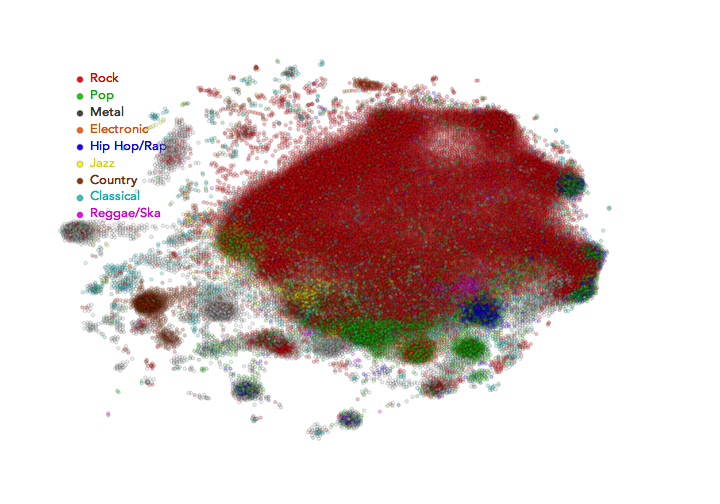
\epsfig{file=img/mystrands_08a_popular_songs_cooccurrences_unsized, width=\textwidth}
\caption{Musical associations in the data set of playlists.}
\label{fig:mystrands_bubbles}
\end{figure}
%

\subsection{Initial data set} % (fold)
\label{sub:noise_removal}

The initial data set is made of 993,825 playlists. % harvested from different Web pages. 
Playlists where any song or artist is repeated often (more than 4 times) are removed for their co-occurrence analysis would lead to the obvious outcome that a song is associated with itself or with other songs by the same artist.

In the set of remaining playlists, 5,433,413 pairs of songs appear contiguously and are not performed by the same artist. 
The most common contiguous pairs of songs are: `Dirty Little Secret' (The All-American Rejects) and `Dance, Dance' (Fall Out Boy); `Grillz' (Nelly) and  `Laffy Taffy' (D4L); `Boulevard Of Broken Dreams' (Green Day) and `Mr Brightside' (The Killers); `My Humps' (Black Eyed Peas) and `Run It!' (Chris Brown); `Caring Is Creepy' (The Shins) and `In The Waiting Line' (Zero 7); `Don't Cha' (Pussycat Dolls) and `Pon De Replay' (Rihanna).

One problem with this data set is that it contains both `good' and `bad' playlists.
People are free to publish on the Web any type of playlists and there is no implicit guarantee that the collected ones are made of songs with an affinity, as listeners can as well create and share random sets of tracks without any meaningful order.
To obtain valid musical associations, bad playlists should be removed from the data set before proceeding with the co-occurrence analysis.
% The next section describes how such playlists are identified and discarded from the data set.

%Since people are free to share any type of playlist on the Web, the data set possibly contains `good' playlists, carefully compiled with a particular purpose, and `bad' playlists, where consecutive songs do not correspond to associated songs. Hereafter, a validation method is described that measures the percentage of consecutive songs in playlists that can comprehensively be considered as associated.

% \subsubsection{Quality of the data set} % (fold)
% \label{ssub:quality_of_the_data_set}
% 
% The significance of each pair of contiguous songs is estimated with a cross-validation process.
% Let $(X,Y)$ be a pair of songs occurring contiguously in a playlist $Q$.
% This pair can either be \emph{significant} or \emph{noisy} meaning that a certain musical association can either exist or not between the two songs.
% If $X$ and $Y$ are indeed associated, then they will also co-occur often in other playlists, while if $Q$ is just a random collection of songs with no particular affinity then this would not happen.
% 
% To test the hypothesis that two songs $X$ and $Y$ are associated, the data set of playlists is partitioned in two: the playlist $Q$ where they co-occur constitutes the \emph{validation data}, while all the other playlists form the \emph{training data} (leave-one-out process).
% 
% The co-occurrence analysis process is performed on the training data to calculate the list of top associated songs with $X$; if $Y$ occurs in this list, then the hypothesis that $X$ and $Y$ are associated is confirmed.
% 
% Formally, let $s_Q: \mathcal{C}^2 \to [0,1]$ be the musical association degree \eqref{eq:final_degree} estimated analysing all the playlists but $Q$ (training data) and let $z_Q(X,Y)$ be the position of $Y$ in the ranked list of top associated tracks according to this degree:
% %
% \begin{equation*}
%  z_Q(X,Y) = \#\{Z \in \mathcal{C}\,|\,s_Q(X,Z) \geqslant s_Q(X,Y) \}\,.        
% \end{equation*}
% %
% If $z_Q(X,Y) = 1$, then $Y$ is the top associated track with $X$ according to the training set, which confirms the hypothesis that the contiguous pair of songs $(X,Y)$ in the validation data is significant.
% 
% If $z_Q(X,Y) \leqslant N$ for a given threshold $N \in \mathbb{N}^+$, then $Y$ is among the top $N$ associated tracks with $X$.
% This can also be seen as a positive validation of the hypothesis as long as $N$ is relatively small.
% If $z_Q(X,Y) > N$, the hypothesis is instead rejected.
% 
% \begin{example}
% A playlist $Q$ in the data set includes `New York, New York' (Frank Sinatra) followed by `Caravan Of Love' (The Housemartins).
% To evaluate whether an association exists between the two songs, the co-occurrence analysis process introduced in Sect.~\ref{sec:co_occurrence_analysis5} is run on all the remaining playlists, obtaining a musical association degree $s_Q$.
% According to this measure, the top associated songs with `New York, New York' (Frank Sinatra) are `The Waters Of March' (Susannah McCorkle), `Stardust' (Glenn Miller) and `New York's My Home' (Sammy Davis Jr.).
% The song `Caravan Of Love' (The Housemartins) only occurs after the first 100 positions.
% In this case, the experience of the people who compiled the remaining playlists rejects the hypothesis that the two songs are indeed associated.    
% \end{example}
% 
% The quality of the entire \emph{data set} of playlists can be measured repeating the same process for every pair of consecutive songs $(X,Y)$ in every playlist $Q$, by first calculating the top associated songs with $X$ from the training data and then verifying whether $Y$ occurs in the first $N$ positions of this list.
% 
% With a threshold of $N = 15$, the number of times the hypothesis is confirmed is 1,467,691, which corresponds to a recall of 27\%. % and is indicative of the 

% paragraph initial_data_set (end)

\subsection{Noise filtering process} % (fold)

Two hypotheses are made for filtering out bad playlists.
The first is that any playlist containing alphabetically ordered songs or artists were probably not compiled with a specific listening purpose (e.g., relaxing, jogging, partying) but as mere groups of consecutive tracks.
The second hypothesis is that neither very short nor very long playlists were created with a purpose that is coherent with the proposed interpretation of playlists.
If these playlists were discarded, then the data set would be reduced to \emph{less} playlists with a \emph{high quality}, that is, playlists which actually contain consecutive associated songs.

The noise filtering process consists in removing from the initial data set any playlist that has less than five songs, more than twenty songs, or has more than five alphabetically ordered songs or artists.
These specific values were determined after having observed the distribution of  alphabetically ordered songs and artists and the distribution of playlist lengths in the initial data set, as illustrated in Fig.~\ref{fig:alphabetical}.
%
\begin{figure}[hbtp]
\centering \setlength{\abovecaptionskip}{3pt}
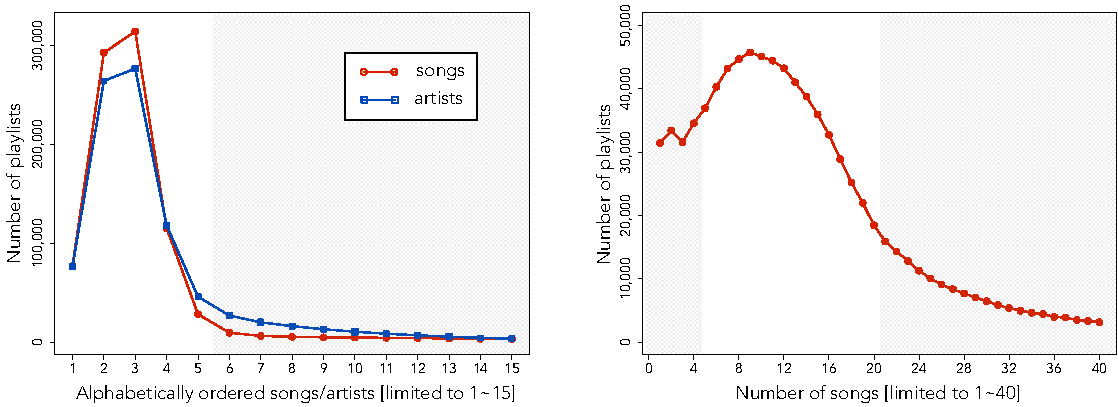
\epsfig{file=img/fig2_2, width=\textwidth}
\caption{Number of playlists with alphabetically ordered songs/artists (left) and with specific lengths (right).}
\label{fig:alphabetical}
\end{figure}

The noise filtering process reduces the data set from 993,825 to 465,438 playlists. The number of contiguous pairs of songs also decreases from 5,433,413 to 1,256,681.
% 
% \subsection{Quality assessment} % (fold)
% \label{sub:quality_of_the_initial_data}
% 
% The rationale of the noise filtering process is that working with less \emph{high quality} playlists is better than working with many \emph{low quality} playlists.
% According to the hypotheses, removing very short, very long and alphabetically ordered playlists can improve the overall quality of the data set.
% The rest of this section evaluates whether these hypotheses hold.
% 
% The first step is to provide a definition of \emph{quality} of a set of playlists. 
% The quality of a set of playlists is the percentage of pairs of songs that occur consecutively in one playlist and, according to the remaining playlists, are musically associated.
% 
% Formally, let $(X,Y)$ be two consecutive songs occurring in a playlist $Q$ and let $s_Q(X,Y)$ be the musical association degree \eqref{eq:final_degree} calculated from the co-occurrences of $X$ and $Y$ in the remaining playlists.
% The more the other playlists where $X$ and $Y$ appear together and the closer their co-occurrences, the higher the value of $s_Q(X,Y)$.
% 
% Let $z_Q(X,Y)$ be the number of songs that are musically associated with $X$ at least as much as $Y$: %, calculated according to all the remaining playlists:
% %
% \begin{equation*}
%  z_Q(X,Y) = \#\{Z \in \mathcal{C}\,|\,s_Q(X,Z) \geqslant s_Q(X,Y) \}\,.        
% \end{equation*}
% %
% If $z_Q(X,Y) \leqslant N$ for a relatively small threshold $N \in \mathbb{N}^+$, then $Y$ is one of the top associated tracks with $X$ according to the remaining playlists. In this case, the analysis of the data set confirms that the contiguous pair $(X,Y)$ corresponds to two associated songs. 
% 
% If $z_Q(X,Y) > N$, then the pair $(X,Y)$ corresponds instead to \emph{noise}: two songs that by chance occur together in one playlist but whose association is not endorsed by the rest of the data set.
% 
% Given these definitions, the quality of the initial data set can be compared with the quality of the filtered data set to test the effectiveness of the noise filtering process. The threshold is fixed to the value of $N = 15$.
% 
% The initial data set contains 5,433,413 pairs of consecutive songs $(X,Y)$; the number of times when $Y$ is confirmed as one of the top $N$ associated tracks with $X$ is 1,467,691.
% 
% Discarding playlists with more than five alphabetically ordered elements reduces these values respectively to 2,710,843 and 765,623. The ratio of these values is 28.2\%, which is 4.5\% higher than the ratio in the initial data set (27\%). This supports the first hypothesis.
% 
% Discarding playlists with less than five or more than twenty songs further reduces the number of pairs of contiguous songs to 1,256,681 and the number of times each pair is confirmed as one of the top $N = 15$ associated to 386,164. The ratio in this case is 30.7\% which is 8.8\% higher than in the initial data set. This supports the second hypothesis.
% %
% 

\section{Tuning parameters} % (fold)
\label{sub:tuning_parameters}

The next step before applying the co-occurrence analysis process to the filtered set of playlists is to decide the values of different parameters introduced in Sect.~\ref{sec:co_occurrence_analysis5}.
The parameters are $\delta$, $\alpha_J$ and $\gamma$, which occur in the functions \eqref{eq:item_association} and \eqref{eq:final_degree}.
These parameters determine how much the distance and the order of songs in playlists influence their association.

\subsection{Tuning the distance parameters} % (fold)
\label{par:considering_separated_songs_}
% [NOTE: These are the results where I also exclude songs that occur in less than 5 playlists, I'm calculating them anew without this filter].

The maximum distance parameter is set to $\delta = 3$, which stands as a compromise between contiguous and distant co-occurrences.
This means that two songs that appear in the same playlist separated by less than three songs are considered as associated, otherwise the association does not subsist.

%The data set includes 1,244,555 pairs of songs that co-occur in a playlist within a distance of $\delta = 3$.

The distance parameters $\alpha_1, \alpha_2, \alpha_3 \in [0,1]$ determine the degree in which closer co-occurrences are more relevant than distant ones.
These parameters are set to $\alpha_1 = 0.6, \alpha_2 = 0.3, \alpha_3 = 0.1$ to gradually assign higher importance to closer co-occurrences.

%The decision about these particular values was taken with a process similar to the one presented in the previous section, comparing for each pair of consecutive songs $(X,Y)$ in the data set the number of times that $Y$ would appear in the list of top $N$ associated tracks with $X$ under different values of $\alpha_1$, $\alpha_2$ and $\alpha_3$.

%The entire data set contains 1,244,555 pairs of songs $(X,Y)$ occurring within a distance of $\delta = 3$ and, with the parameters set to  $\alpha_1 = 0.6, \alpha_2 = 0.3, \alpha_3 = 0.1$, the number of times that $Y$ is found in the list of top $N = 15$ associated ones with $X$ is 387,313. %, corresponding to a ratio of 30.8\%.

%On the contrary, considering only adjacent co-occurrences (that is, setting the parameters to $\alpha_1 = 1, \alpha_2 = \alpha_3 = 0$) would result in a lower number of 386,184 pairs. % of consecutive songs identified as associated, with a ratio of 30.7\%.
%
%Similarly, assigning the same importance to co-occurrences at different distances ($\alpha_1 = \alpha_2 = \alpha_3 = \frac{1}{3}$) would result in only 357,232 pairs of associated songs. %, with a smaller ratio of 28.4\%.

% paragraph considering_separated_songs_ (end)

% $\frac{357,232}{15*1,224,555} = 1.94\%$, while the case of $\beta = 0.5$ makes me predict the right successor in 387,313 cases with N = 15, which gives a precision of $\frac{387,313}{15*1,224,555} = 2.11\%$, which is (a 2.4\%) higher than before. So considering different distances makes sense.

\subsection{Tuning the order parameter} % (fold)
\label{par:considering_different_orderings_}

%The more two songs $(X,Y)$ occur in the same order, the more they go well together in that order.
The parameter $\gamma \in [0,0.5]$ determines the degree in which inverse co-occurrences ($X$ \emph{after} $Y$) also contribute to determine their associations.
%
In this case, this parameter is set to $\gamma = 0.2$: direct co-occurrences (where $X$ occurs \emph{before} $Y$) are identified as more relevant to determine the association between $X$ and $Y$ than inverse co-occurrences.

%As for the distance parameters, this value was decided after comparing different possible scenarios. % and selecting the one which returned the highest ratio of consecutive songs identified as associated.
%
%With the parameter set to $\gamma = 0$, the number of consecutive pairs of songs $(X,Y)$ for which $Y$ results in the list of top $N = 15$ associated tracks with $X$ is 387,313.

%On the contrary, assigning the same importance to direct and inverse co-occurrences ($\gamma = 0.5$) would result in a smaller value of 347,362.
%Assigning a slighter large influence to direct than to inverse co-occurrences ($\gamma = 0.25$) would also return a smaller value (372,995).

Setting the parameter to $\gamma = 0.2$ expresses the fact that the order in which two songs occur in playlists has an effect on the measure of their association. 
This value was decided observing that many playlists in the data set are \emph{asymmetric} by nature: songs sound well together in one direction but not necessarily in the other one. 
This can be explained by the fact that several authors, especially disc jockeys, compile playlists where the \emph{end} of each song mixes with the \emph{beginning} of the next one.
In these cases, the order should be accounted for when measuring associations.



% \subsection{Distance and order of co-occurrences} % (fold)
% \label{sub:tuning_parameters}
% 
% The noise filtering process has identified, within the initial data set of playlist, a subset of `good' playlists on which to apply the co-occurrence analysis process described in Sect.~\ref{sec:co_occurrence_analysis5} to measure musical associations.
% 
% Before running the analysis, the values of the parameters $\delta$, $\alpha_J$ and $\gamma$ that occur in the functions \eqref{eq:item_association} and \eqref{eq:final_degree} have to be decided, indicating how much the distance and the order of songs in playlists influence their association.
% 
% \subsubsection{Tuning the distance parameters} % (fold)
% \label{par:considering_separated_songs_}
% 
% The maximum distance is set to $\delta = 3$, a compromise between contiguous and distant co-occurrences. Songs that occur in the same playlist separated by more than three songs are not considered as associated.
% 
% In order to gradually assign more importance to closer co-occurrences, the distance parameters $\alpha_1, \alpha_2, \alpha_3 \in [0,1]$ are set to the values $\alpha_1 = 0.6, \alpha_2 = 0.3, \alpha_3 = 0.1$.
% 
% \subsubsection{Tuning the order parameter} % (fold)
% \label{par:considering_different_orderings_}
% 
% The order parameter $\gamma \in [0,0.5]$ determines the degree in which inverse co-occurrences ($X$ \emph{after} $Y$) also contribute to determine their associations.
% This parameter is set to $\gamma = 0.2$ to assign only a small importance to inverse co-occurrences.
% The motivation is that playlists are often not symmetric.
% Songs can be ordered with a specific purpose that does not hold if reversed, for instance when the end of a song mixes well with the beginning of the next one.
% 



\section{The resulting associations} % (fold)
\label{sub:the_smoothness_degrees_we_obtain}

%Filtering out alphabetically ordered playlists and playlists that are too short or long improves the quality of the data set with respect to the musical associations. Considering separated songs with decreasing weights according to the distance is also important, while considering co-occurrences in both orders does not seem relevant.

Having filtered noise from the initial data set of 993,825 playlists and having applied the co-occurrence analysis technique with the parameters set to:
\begin{itemize}
 \item maximum distance between songs: $\delta = 3$,
 \item degrees in which distance influences the strength of the association: $\alpha_1 = 0.6, \alpha_2 = 0.3, \alpha_3 = 0.1$,
 \item degree in which popularity bias is punished:  $\beta = 0.8$,
 \item degree in which order influences %the strength of 
 the association: $\gamma = 0.2$,
 \item degrees in which different types of co-occurrences influence the strength of the association: $\phi_1 = 0.6, \phi_2 = 0.3, \phi_3 = 0.1$,
\end{itemize}
the association degrees $s(X,Y)$ defined in Sect.~\ref{sec:co_occurrence_analysis5} are finally calculated.

Associations between songs by the same artist are excluded for their obviousness, as well as songs by `virtual' artists (such as `Various Artists' or `Soundtrack') and songs appearing in less than 5 playlists, for their minimal statistical significance.
This threshold was fixed observing how the popularity of songs distributes in the data set of playlists (Fig.~\ref{fig:lengths}).
%
\begin{figure}[hbtp]
\centering \setlength{\abovecaptionskip}{3pt}
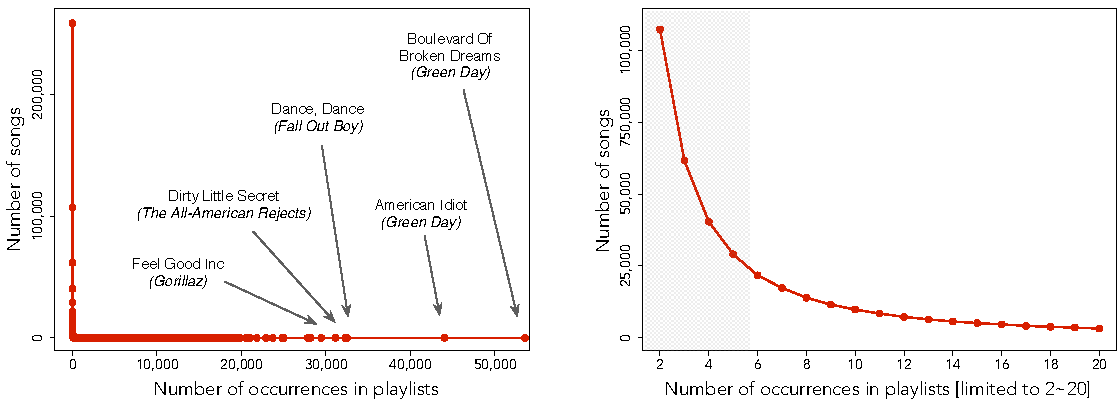
\epsfig{file=img/fig2_3, width=\textwidth}
\caption{Occurrences per songs in retrieved playlists.}
\label{fig:lengths}
\end{figure}

Eventually, a musical association degree $s(X,Y)$ was estimated for as many as 46,217,300 % this includes artist-to-artist
distinct pairs of 415,498 songs by 47,148 distinct artists.

%Two examples of musical associations found for a given song and artists are presented hereafter. %; other examples are reported with their evaluation in Chap.~\ref{cha:evaluation}.

% \begin{example}\label{ex:flymetothemoon}
% The song `Fly Me To The Moon' (Astrud Gilberto) occurs in 364 playlists. % compiled by MusicStrands members.
% The analysis finds out that 182 songs appear in playlists with `Fly Me To The Moon', that 52 songs appear in playlists with other songs by Astrud Gilberto, and that 194 songs are from artists appearing in playlists with songs by Astrud Gilberto.
% The co-occurrence analysis allows to rank all these songs according to how much they are associated with `Fly Me To The Moon', uncovering the following songs as the top associated: `Come Fly With Me' (Frank Sinatra), `L-O-V-E' (Nat King Cole), `What A Wonderful World' (Louis Armstrong), `I've Got The World On A String' (Frank Sinatra), `Ain't That A Kick In The Head' (Dean Martin), `Beyond The Sea' (Bobby Darin), `At Last' (Etta James) and `Kissing A Fool' (Michael Bubl\'{e}).
% \end{example}
% 
% \begin{example}
% Songs from the band Panic!\;At The Disco occur in 29,052 playlists.
% The analysis finds out that songs by 5,170 distinct artists appear in playlists with any song by Panic!\;At The Disco and rank their artists according to how much they are musically associated with Panic!\;At The Disco.
% The following artists are uncovered as the most associated: October Fall, Pilot Speed, My American Heart, Nightmare Of You, The Presets, The Pink Spiders and Junior Boys.
% % NOTE: ADD MySpace links to all these groups!!
% \end{example}
% 

\subsection{Evaluating song associations} % (fold)
\label{sub:evaluating_song_association}

Given a song $X$ in the data set, the songs $Y$ with the highest association degree $s(X,Y)$ are the songs that go best in a sequence after $X$ according to the human experience recorded in playlists.
The following is an example of list of top associated tracks.

\begin{example}\label{ex:newyork}
The song `New York, New York' (Frank Sinatra) occurs in 219 playlists.
The analysis finds that 173 distinct songs appear in playlists with `New York, New York', that 6,458 songs appear in playlists with other songs by Frank Sinatra, and that 26,402 songs are from artists appearing in playlists with songs by Frank Sinatra.
The co-occurrence analysis allows to rank all these songs according to how much they are associated with `New York, New York', uncovering the following songs as the top associated ones:  `The Waters Of March' (Susannah McCorkle), `Stardust' (Glenn Miller), `New York's My Home' (Sammy Davis Jr.), `Manhattan Avenue' (Nellie McKay), `Mississippi Goddam' (Nina Simone), `Something Beautiful' (Robbie Williams).
\end{example}

The example highlights some common properties of the lists of top associated songs.
The first characteristic is that the top songs are not particularly famous, yet share a strong affinity with the seed track.
 `The Waters Of March' (Susannah McCorkle), for instance, is strongly connected with `New York, New York' (Frank Sinatra) since they were both composed in the Seventies and performed as musical standards by various singers.
The reason why uncommon songs appear higher in the list is the high value of the popularity bias parameter $\beta = 0.8$ which punishes songs that occur very often in the set of playlists.

Another positive characteristic of the list is diversity: all the songs are performed by different artists and belong to multiple genres and periods; `Something Beautiful' (Robbie Williams), for instance, was published in 2003.


\subsection{Evaluating artist association} % (fold)

As well as lists of top associated tracks, the co-occurrence analysis can produce lists of top associated artists.
Given an artist $a(X)$ in the data set, the artists whose songs have in average the highest association degree with the songs of $a(X)$ are the top associated artists with $a(X)$.

Working at the level of artists is not as specific as working at the level of songs: two songs can go well together for acoustic reasons (same timbre, rhythm, lyrics) while a correlation between two artists is more abstract, implying some sort of social or cultural relationships (e.g., two artists are contemporary, play the same instrument, have collaborated, belong to the same genre).
An example of list of top associated artists is reported hereafter.

\begin{example}
Themes written by the soundtrack composer John Williams appear in 2,367 playlists.
The analysis finds out that songs by 866 distinct artists appear in playlists with any track by John Williams. These artists are ranked according to how much they are musically associated with John Williams;
the following artists are uncovered as the most associated: Itzhak Perlman, Christopher Young, Arthur Fiedler, London Symphony Orchestra, John Debney, Danny Elfman, John Carpenter, John Barry.
% NOTE: ADD MySpace links to all these groups!!
\end{example}

Similarly to Example~\ref{ex:newyork}, an interesting property of this list is that uncommon but strongly associated items appear first, followed by more popular ones.
Itzhak Perlman, for instance, is not a soundtrack composer but a violinist who played first violin in `Schindler's List' soundtrack, composed by John Williams.
Arthur Fiedler also shares a strong affinity with John Williams, who took his place as the conductor of the Boston Pops orchestra in 1979 after Fiedler's death.
John Debney, Danny Elfman and John Barry are award-winning movie composers contemporary to John Williams.

\subsection{Comparisons with other music similarity measures} % (fold)
\label{sub:comparisons_with_music_similarity_measures}

%The lists of top associated songs and artists obtained point out which items are more indicate to be played in sequence.
For the purpose of evaluation, some lists of top associated songs and artists are hereafter contrasted with equivalent lists calculated with distinct sources of musical knowledge obtained from different Web sites.
The Web sources used for the comparison are: Yahoo! Music, Last.fm and Audiobaba for associated songs and All Music Guide, Yahoo! Music, Last.fm, MusicStrands and MusicSeer for associated artists.
The technique presented in this chapter does not exactly look for `similar' songs, but for songs that go well together in sequence.
Nevertheless, comparing its assessments with those offered by other techniques can reveal interesting peculiarities.

Yahoo! Music makes available for each song and artist in its catalogue a list of similar tracks and artists ``generated from end user feedback'' \cite{Baumann04}.
Last.fm offers for each song a Web page listing what people who listened to that song also listened to.
Audiobaba uses a content-based approach: for each song, a list of tracks that are acoustically similar is returned.

For associations among artists, All Music Guide includes handcrafted contributions written by expert editors and is considered as the `bible' of music reviews, the ground truth for music classification research \cite{Pachet00b,Hu07,Magno08,Sordo08}.
MusicStrands derives associations from the same data set of playlists employed in this dissertation, but applying a different technique based on ``bags of associations'' \cite{Shur06}.
MusicSeer follows two different approaches: one is based on a survey to collect subjective judgements about artist similarity, the other one on playlist co-occurrences. 
The MusicSeer survey includes associations for about 413 artists \cite{Logan03}, while the playlist-based approach reports associations between 60,931 artists from the analysis of 29,164 playlists retrieved from Art Of The Mix \cite{Ellis03}.

Tables~\ref{table:samplerelevance}, \ref{table:samplerelevance2} and~\ref{table:samplerelevance3} report the most associated tracks for the songs `New York, New York' (Frank Sinatra), `Whenever, Wherever' (Shakira) and `Smoke On The Water' (Deep Purple).
Tables~\ref{table:samplerelevance4}, \ref{table:samplerelevance5}, \ref{table:samplerelevance6} and \ref{table:samplerelevance7} compare the top artists delivered for John Williams, Frank Sinatra, Abba and Destiny's Child. 

\begin{table}[bthp]\centering
\setlength{\extrarowheight}{3pt}
\setlength{\abovecaptionskip}{3pt}
\setlength{\belowcaptionskip}{3pt}
\setlength{\intextsep}{0pt}
\caption{Top associated songs for `New York, New York' (Frank Sinatra).}\label{table:samplerelevance}
{\fontsize{8}{10}\selectfont
\begin{tabular}{|c|p{0.8\textwidth}|}
 \hline 
 \multirow{3}{*}{Poolcasting} &
 `The Waters Of March' (Susannah McCorkle), `Stardust' (Glenn Miller), `New York's My Home' (Sammy Davis Jr.), `Manhattan Avenue' (Nellie McKay), `Mississippi Goddam' (Nina Simone), `Something Beautiful' (Robbie Williams) \vspace{2pt} \\
 \hline
 \multirow{3}{*}{Yahoo!} &
 `Piano Man' (Billy Joel), `That's Amore'	(Dean Martin), `At Last' (Etta James), `Mrs. Robinson'	(Simon \& Garfunkel), `The Boxer' (Simon \& Garfunkel), `Bridge Over Troubled Water' (Simon \& Garfunkel) \vspace{2pt} \\
 \hline
 \multirow{3}{*}{Last.fm} &
 `Strangers In The Night' (Frank Sinatra), `Fly Me To The Moon'	(Frank Sinatra), `What A Wonderful World' (Louis Armstrong), `Walkin' My Baby Back Home'	(Nat King Cole), `Try To Remember' (Bobby Darin), `Beyond The Sea' (Bobby Darin) \vspace{2pt} \\
 \hline
 \multirow{3}{*}{Audiobaba} &
 `Woman, Woman' (Gary Puckett), `Spirit In The Night'	(Bruce Springsteen), `You Make Me Feel So Young' (Frank Sinatra), `Mud On The Tires'	(Brad Paisley), `Lucky To Be Here' (Montgomery Gentry), `6 AM' (Random Access) \vspace{2pt} \\
 \hline
 \noalign{\bigskip}
\end{tabular}}
\end{table}
%{\setlength{\intextsep}{0pt}
\begin{table}[bthp]\centering
\setlength{\extrarowheight}{3pt}
\setlength{\abovecaptionskip}{3pt}
\setlength{\belowcaptionskip}{3pt}
\caption{Top associated songs for `Whenever, Wherever' (Shakira).}\label{table:samplerelevance2}
{\fontsize{8}{10}\selectfont\begin{tabular}{|c|p{0.8\textwidth}|}
 \hline
 \multirow{3}{*}{Poolcasting} &
 `You Spin Me Round' (Thal\'{\i}a), `Crazy In Love' (Beyonc\'{e} \& Jay-Z), `Grazing In the Grass' (Raven-Symon\'{e}), `Si Ya Se Acab\'{o}' (Jennifer Lopez), `Freakout' (B*Witched), `Perros' (Paulina Rubio) \vspace{2pt} \\ 
 \hline
 \multirow{3}{*}{Yahoo!} &
 `Baby One More Time'	(Britney Spears), `Irresistible'	(Jessica Simpson), `If You Had My Love' (Jennifer Lopez), `Candy'	(Mandy Moore), `Bye Bye Bye'	('N Sync), `Genie In A Bottle' (Christina Aguilera) \vspace{2pt} \\
 \hline
 \multirow{3}{*}{Last.fm} &
 `Underneath Your Clothes'	(Shakira), `Objection (Tango)'	(Shakira), `Radar' (Britney Spears), `Keeps Gettin' Better'	(Christina Aguilera), `Beautiful Liar'	(Beyonc\'{e} feat. Shakira), `Waiting for Tonight' (Jennifer Lopez) \vspace{2pt} \\
 \hline
 \multirow{3}{*}{Audiobaba} &
 `Too Bad'	(Bad Company), `Sunday Girl'	(Erasure), `Life In The Fast Lane' (Eagles), `These Dreams Of You Are So Much Sweeter Than The Truth'	(The Sharp Things), `Powerful Thing'	(Trisha Yearwood), `Migration' (Jimmy Buffett) \vspace{2pt} \\
 \hline
\end{tabular}}
\end{table}
%}
%{\setlength{\intextsep}{0pt}
\begin{table}[bthp]\centering
\setlength{\extrarowheight}{3pt}
\setlength{\abovecaptionskip}{3pt}
\setlength{\belowcaptionskip}{3pt}
\caption{Top associated songs for `Smoke On The Water' (Deep Purple).}\label{table:samplerelevance3}
{\fontsize{8}{10}\selectfont\begin{tabular}{|c|p{0.8\textwidth}|}
 \hline
 \multirow{3}{*}{Poolcasting} &
 `Silver Machine' (Hawkwind), `The Joker' (Steve Miller Tribute Band), `Dream Evil' (Dio), `Rock N' Roll Hoochie Koo' (Johnny Winter), `South Saturn Delta' (Jimi Hendrix), `Nottingham Lace' (Buckethead) \vspace{2pt} \\ 
 \hline
 \multirow{3}{*}{Yahoo!} &
 `Melissa'	(The Allman Brothers Band), `Surrender'	(Cheap Trick), `Sweet Talkin' Woman' (Electric Light Orchestra), `Somebody To Love'	(Jefferson Airplane), `White Rabbit'	(Jefferson Airplane), `Maggie May' (Maggie May) \vspace{2pt} \\
 \hline
 \multirow{3}{*}{Last.fm} &
 `Highway Star'	(Deep Purple), `Child in Time'	(Deep Purple), `Stairway to Heaven' (Led Zeppelin), `Paranoid'	(Black Sabbath), `Whole Lotta Love'	(Led Zeppelin), `Black Dog' (Led Zeppelin) \vspace{2pt} \\
 \hline
 \multirow{3}{*}{Audiobaba} &
 `Double E'	(Neil Young), `This Can't Be Love'	(Freeborn), `The Lady' (TheHookUp), `Elegant People'	(Jaco Pastorius Big Band), `Last Chance'	(Ear Candy), `Diggers Of Ditches Everywhere' (These Arms Are Snakes) \vspace{2pt} \\
 \hline
\end{tabular}}
\end{table}
%}
%{\setlength{\intextsep}{0pt}
\begin{table}[bhtp]\centering
\setlength{\extrarowheight}{3pt}
\setlength{\abovecaptionskip}{3pt}
\setlength{\belowcaptionskip}{3pt}
\setlength{\intextsep}{0pt}
\caption{Top associated artists for John Williams.}\label{table:samplerelevance4}
{\fontsize{8}{10}\selectfont
\begin{tabular}{|c|p{0.8\textwidth}|}
 \hline 
 \multirow{2}{*}{Poolcasting} &
 Itzhak Perlman, Christopher Young, Arthur Fiedler, London Symphony Orchestra, John Debney, Danny Elfman, John Carpenter, John Barry \vspace{2pt} \\
 \hline
 \multirow{2}{*}{MusicStrands} &
 Danny Elfman, Vangelis, Hollywood Studio Orchestra, Erich Kunzel, Green Day, Gorillaz, Weird Al Yankovic, John Barry, Queen, Eminem \vspace{2pt} \\
 \hline
 AllMusic &
 John Barry, Jerry Goldsmith, Elmer Bernstein, Howard Shore, Erich Korngold \vspace{2pt} \\
 \hline
 \multirow{2}{*}{Yahoo!} &
 Franz Joseph Haydn, James Newton Howard, Michael Kamen, National Philarmonic Orchestra, Alan Silvestri, Jerry Goldsmith, John Barry \vspace{2pt} \\
 \hline
 \multirow{2}{*}{Last.fm} &
 Jerry Goldsmith, James Horner, Patrick Doyle, Alan Silvestri, James Newton Howard, Howard Shore, Hans Zimmer, Nicholas Hooper, Danny Elfman \vspace{2pt} \\
 \hline
 \noalign{\bigskip}
\end{tabular}}
\end{table}
%}
%{\setlength{\intextsep}{0pt}
\begin{table}[bhtp]\centering
\setlength{\extrarowheight}{3pt}
\setlength{\abovecaptionskip}{3pt}
\setlength{\belowcaptionskip}{3pt}
\setlength{\intextsep}{0pt}
\caption{Top associated artists for Frank Sinatra.}\label{table:samplerelevance5}
{\fontsize{8}{10}\selectfont
\begin{tabular}{|c|p{0.8\textwidth}|}
 \hline 
 \multirow{2}{*}{Poolcasting} &
 Dean Martin, Sammy Davis Jr., Judy Garland, Bing Crosby, The California Raisins, Tony Bennett, Louis Prima, Rosemary Clooney, Nat King Cole \vspace{2pt} \\
 \hline
 \multirow{2}{*}{MusicStrands} &
 Dean Martin, Billie Holiday, Nat King Cole, Perry Como, Ella Fitzgerald, Andy Williams, Tony Bennett, Etta James, Bing Crosby, Diana Krall \vspace{2pt} \\
 \hline
 \multirow{2}{*}{AllMusic} &
 Dean Martin, Vic Damone, Dick Haymes, Sarah Vaughan, Nat King Cole, Dinah Washington, Mel Torm\'{e}, Ella Fitzgerald, Tony Bennett, Jo Stafford \vspace{2pt} \\
 \hline
 \multirow{2}{*}{Yahoo!} &
 Dean Martin, Tony Bennett, Nat King Cole, Ray Charles, The Beach Boys, Simon \& Garfunkel, Elvis Presley, The Beatles, Norah Jones, Norah Jones  \vspace{2pt} \\
 \hline
 \multirow{2}{*}{Last.fm} &
 Dean Martin, Sammy Davis, Jr., Frank Sinatra \& Tommy Dorsey, Tony Bennett, Nat King Cole, Bobby Darin, Ella Fitzgerald, Mel Torm\'{e} \vspace{2pt} \\
 \hline
 \multirow{2}{*}{MS Survey} &
 Eric Clapton, Billy Joel, Elton John, Elvis Costello, Elvis Presley, Van Morrison, John Lennon, Bob Dylan, Nine Days, Ozzy Osbourne \vspace{2pt} \\
 \hline
 \multirow{2}{*}{MS Playlists} &
 Elvis Presley, Elton John, John Denver, Abba, Whiskeytown, Beatles, Billy Joel, Bob Marley, Eric Clapton, Everly Brothers \vspace{2pt} \\
 \hline
 \noalign{\bigskip}
\end{tabular}}
\end{table}
%}
\begin{table}[bhtp]\centering
\setlength{\extrarowheight}{3pt}
\setlength{\abovecaptionskip}{3pt}
\setlength{\belowcaptionskip}{3pt}
\setlength{\intextsep}{0pt}
\caption{Top associated artists for Abba.}\label{table:samplerelevance6}
{\fontsize{8}{10}\selectfont
\begin{tabular}{|c|p{0.8\textwidth}|}
 \hline 
 \multirow{2}{*}{Poolcasting} &
 Agnetha F\"{a}ltskog, A-Teens, Chic, Gloria Gaynor, The 5th Dimension, Andy Gibb, Olivia Newton-John, Rose Royce, KC \& The Sunshine Band, Bee Gees \vspace{2pt} \\
 \hline
 \multirow{2}{*}{MusicStrands} &
 Donna Summer, Madonna, Gloria Gaynor, Cyndi Lauper, Blondie, Kool \& The Gang, Elton John, The B-52s, Michael Jackson, Diana Ross \vspace{2pt} \\
 \hline
 \multirow{2}{*}{AllMusic} &
 Ambsoris, Olivia Newton-John, The Carpenters, Captain \& Tennille, Bucks Fizz, Fletwood Mac, Andy Gibb, Lindsey Buckingham, The Cowsills \vspace{2pt} \\
 \hline
 \multirow{2}{*}{Yahoo!} &
 Bee Gees, The Carpenters, Elvis Presley, The Beatles, Foreigner, Whitney Houston, Bon Jovi, Madonna, Barry Manilow, Michael Jackson \vspace{2pt} \\
 \hline
 \multirow{2}{*}{Last.fm} &
 Agnetha F\"{a}ltskog, Frida, Boney M., Bee Gees, Olivia Newton-John, Baccara, Cher, Bucks Fizz, Donna Summer, Army of Lovers, Alcazar \vspace{2pt} \\
 \hline
 \multirow{2}{*}{MS Survey} &
 Ace of Base, Bee Gees, Blondie, Spice Girls, Olivia Newton-John, Beach Boys, Roxette, Cyndi Lauper, Backstreet Boys, Donna Summer \vspace{2pt} \\
 \hline
 \multirow{2}{*}{MS Playlists} &
 Bee Gees, Blondie, Cyndi Lauper, Queen, Cat Stevens, Cher, Beach Boys, Donna Summer, Olivia Newton-John, Phil Collins \vspace{2pt} \\
 \hline
 \noalign{\bigskip}
\end{tabular}}
\end{table}
%
%{\setlength{\intextsep}{0pt}
\begin{table}[bhtp]\centering
\setlength{\extrarowheight}{3pt}
\setlength{\abovecaptionskip}{3pt}
\setlength{\belowcaptionskip}{3pt}
\setlength{\intextsep}{0pt}
\caption{Top associated artists for Destiny's Child.}\label{table:samplerelevance7}
{\fontsize{8}{10}\selectfont
\begin{tabular}{|c|p{0.8\textwidth}|}
 \hline 
 \multirow{2}{*}{Poolcasting} &
 Kelly Rowland, City High, Ciara, Fantasia, Christina Milian, Beyonc\'{e}, Ashanti, Girls Aloud, 3LW, Dru Hill \vspace{2pt} \\
 \hline
 \multirow{2}{*}{MusicStrands} &
 Ciara, Pussycat Dolls, Usher, Beyonc\'{e}, Nelly, 50 Cent, Mariah Carey, Chris Brown, Gwen Stefani, Eminem \vspace{2pt} \\
 \hline
 \multirow{2}{*}{AllMusic} &
 Toni Braxton, Mariah Carey, Jennifer Lopez, Aaliyah, Xscape, Ginuwine, Deborah Cox, Kelly Price, Faith Evans, Brandy, Usher, Mya \vspace{2pt} \\
 \hline
 \multirow{2}{*}{Yahoo!} &
 Faith Evans, Cruel Story Of Youth, Nich Lachey, Jamie Foxx, Jessica Simpson, Ciara, Jagged Edge, Lil' Kim, Ryan Cabrera, Janet Jackson \vspace{2pt} \\
 \hline
 \multirow{2}{*}{Last.fm} &
 Beyonc\'{e}, Kelly Rowland, Michelle Williams, LeToya, Solange, Ashanti, Ciara, Brandy, Mariah Carey, Monica, Aaliyah, TLC, Mya \vspace{2pt} \\
 \hline
 \noalign{\bigskip}
\end{tabular}}
\end{table}
%}
%

The analysis of these lists of top associated songs does not reveal a great diversity among different musical sources, although some peculiarities can be observed.
As noted previously, co-occurrence analysis of playlists can identify songs that are associated but not overly popular, something that does not happen with every other technique.
Yahoo! Music, for instance, returns the famous hit `Baby One More Time' (Britney Spears) as the top associated song for `Whenever, Wherever' (Shakira). For this song, `You Spin Me Round' (Thal\'{\i}a) is possibly a better match since both songs were released in 2001 and performed by Latin American singers (see Table~\ref{table:samplerelevance2}).
Another observation is that Last.fm and Yahoo! Music have limited diversity in the results: Last.fm returns two tracks by Frank Sinatra as the top associated for `New York, New York' (see Table~\ref{table:samplerelevance}) while Yahoo! Music repeats songs by the same artists  (Simon \& Garfunkel in Table~\ref{table:samplerelevance} and Jefferson Airplane in Table~\ref{table:samplerelevance3}).

The analysis of top associated artists also reveals particular behaviours for the different methods.
First, almost every source of knowledge yields Dean Martin as the top associated artist with Frank Sinatra (see Table~\ref{table:samplerelevance5}), marking a clear affinity between the two.
Next, the playlist-based approach introduced in this chapter returns first artists that are not very popular but strongly associated.

An example is provided by Table~\ref{table:samplerelevance6} where Agnetha F\"{a}ltskog shows up as the top associated artist for Abba according to the co-occurrence analysis of playlists. 
Agnetha F\"{a}ltskog is not a very famous solo artist but she is indeed popularly known as the lead singer of Abba.
Similarly, Table~\ref{table:samplerelevance7} shows Kelly Rowland (one of the members of Destiny's Child) as one of the top associated artist with Destiny's Child.

This behaviour is possibly the most distinct advantage of the playlist-based method: to be able to spot out items that share a strong social affinity. % better than items that just happen to be very popular.
This result is obtained from the automatic analysis of playlists, without human intervention.
All Music Guide, on the other hand, requires man-hours of dedicated expert work to obtain results that are almost equivalent in terms of affinity and sometimes worse in terms of diversity.

% This effect is mainly produced by the popularity bias parameter set to $\beta = 0.8$ that pushes down in the list artists that are over-popular in the set of analysed playlists.
% 
% 
% %\paragraph{Observations.} % (fold)
% %\label{par:observations_}
% 
% The proposed technique tends to return top associated songs that are generally not as popular as those returned by other methods.
% Susannah McCorkle, for instance, is probably not as famous as Billy Joel or Frank Sinatra (see Table~\ref{table:samplerelevance}), still her version of `The Waters of March'\,---a bossa nova standard\,---\,has a strong musical association with `New York, New York'.
% Likewise, Thal\'{\i}a's version of `You Spin Me Round' is not as famous as `Baby One More Time' (Britney Spears) (see Table~\ref{table:samplerelevance2}) but is possibly more musically associated with `Whenever, Wherever' (Shakira), since both songs were performed by Latin American singers and released in 2001.
% 
% In general, the proposed technique shows first songs that are strongly associated although not very popular, followed by songs that are more popular, such as `Crazy In Love' (Beyonc\'{e} \& Jay-Z) in Table~\ref{table:samplerelevance2}.
% This behaviour is the direct consequence of the popularity bias parameter set to $\beta = 0.8$; with a lower value, over-popular songs would show up earlier in the list.
% 
% Another observation is how most of the top associated tracks according to playlist co-occurrences `sound similar', although no acoustic-based analysis has been performed.
% Moreover, in all three examples, Last.fm returns tracks by the same artists as the most associated, while the proposed technique explicitly avoids this kind of outcome for its obviousness.
% Diversity among the results is also important; as a matter of fact all the top associated songs returned are performed by different artists while Yahoo! Music tends instead to repeat the same artists in the list of similar songs (Simon \& Garfunkel in Table~\ref{table:samplerelevance} and Jefferson Airplane in Table~\ref{table:samplerelevance3}).
% 
% % paragraph observations_ (end)
% 
% 
% \subsection{Evaluating artist association} % (fold)
% 
% The artist-to-artist association function \eqref{eq:artist_to_artist} identifies associated artists whose songs go well together in sequence.
% 
% Lists of top associated artists calculated with the function  \eqref{eq:artist_to_artist} are compared hereafter with the lists of most similar artists retrieved from the following music sources: All Music Guide, Yahoo! Music, Last.fm, MusicStrands and MusicSeer.
% 
% 
% 
% 
% %\paragraph{Observations.} % (fold)
% %\label{par:observations2}
% 
% As for song-to-song associations, the proposed technique is able to spot out, as top associated, artists that are not extremely popular but share a strong relationship with the seed artist.
% Agnetha F\"{a}ltskog, for instance, is not a very famous solo artist but is popularly known as the lead singer of Abba (see Table~\ref{table:samplerelevance4}); Itzkah Perlman played first violin in `Schindler's List' soundtrack, directed by John Williams (see Table~\ref{table:samplerelevance5}); Kelly Rowland was a member of the band Destiny's Child (see Table~\ref{table:samplerelevance6}).
% %
% This effect is mainly produced by the popularity bias parameter set to $\beta = 0.8$ that pushes down in the list artists that are over-popular in the set of analysed playlists.
% 
% Another interesting observation is how, in the case of Frank Sinatra, most techniques return Dean Martin as the top associated artist (see Table~\ref{table:samplerelevance7}), although based on different types of knowledge.
% 
% The proposed technique also behave well when compared to All Music Guide, which is often considered as a base referrer for its associations are compiled by hands by a group of experts.
% The main advantage of the proposed technique is that it is autonomous and scalable, while All Music Guide requires many man-hours to obtain similar results.
% 
% % after Fiedler's death in 1979, the conductorship of the Boston Pops was taken over by John Williams.
% 

% paragraph observations2 (end)

% section the_experiments2 (end)

\section{Summary} % (fold)
\label{sub:summing_up3}

This chapter has presented a technique to measure the associations that exist between any two songs and artists.
Associations are estimated observing how millions of persons organise music for their daily activities.

The technique consists in collecting a large amount of playlists from the Web and analysing the co-occurrences of songs, under the idea that the more two songs occur together and closely, the stronger their association.

Playlists are expressions of human experiences and include factual knowledge about how people listen to music. Playlists are ordered sequences of songs associated for acoustic, cultural or social reasons that cannot be completely uncovered by experts or content-based methods.

The proposed method analyses, for each pair of songs $(X,Y)$, the number of playlists where they both appear, their order, distance, popularity and the co-occurrences of their artists and obtains a measure $s(X,Y) \in [0,1]$ of their musical association.

This method has been applied to a real data set of about a million playlists retrieved from multiple Web-based music communities.
The result has been the estimation of musical associations for 415,498 distinct songs from 47,148 artists.
%
For each song and artist, a list of top associated items can be compiled.
These lists tend to show first items that are not very popular but strongly associated with the seed item, followed by more popular ones.

Some of these lists have been compared with equivalent ones gathered from music-related Web services such as All Music Guide and Last.fm.
The comparison has shown results that are quite equivalent independently of the source of knowledge used.
The main advantages of the automatic technique introduced in this chapter are its scalability and the ability to spot out artists with a strong social affinity (Agnetha F\"{a}ltskog for Abba, Kelly Rowland for Destiny's Child), a property not found in the expert-based knowledge of All Music Guide.

The musical associations estimated in this chapter will be employed in the poolcasting technique introduced in Chap.~\ref{cha:poolcasting_web_radio} to determine which songs to play in a musical sequence to guarantee a sense of continuity from one song to the next.

%Chap.NN will explain how this musical association degree is used by poolcasting to create music channels where each song musically flows after the previous one.

% section summing_up3 (end)

% chapter smoothness (end)

\chapter{Individual listening behaviours} % (fold)
\label{cha:preferences}
\songquote{I know just what you need\\
I might just have the thing}{Soul Asylum, 1995} 
\section{Music libraries and listening habits} % (fold)
\label{sec:listening_behaviour}

% The previous chapter has made clear that Internet holds a deep knowledge of the way in which people experience music and that this knowledge can be automatically retrieved and analysed to better understand the associations that subsist between songs and artists.

Different persons are characterised by different listening behaviours: some are used to play all kinds of music in a shuffled order, others to listen only to a particular genre; some are eager to discover the latest trends of contemporary music, others are obsessed with playing the same album again and again.

The previous chapter focused on music organised in playlists.
Some persons do not use playlists at all but decide in real time which songs to play in their music devices.
The simple fact of a person picking a particular song to play is already a musical experience that is worth be analysed.

The wide proliferation of digital music players has made it easy to track the history of a listener.
Most digital players (Apple iTunes, iPod, Winamp, Windows Media Player, etc.) store data about each played song; Apple iTunes, for instance, records the play count (number of times the song was played), the play recency (last time the song was played), the skip count (number of times the song was skipped before its end) and the user rating for each song in the music library (see Fig.~\ref{fig:itunes_claudio}).
%
\begin{figure}[bthp]
\centering \setlength{\abovecaptionskip}{3pt}
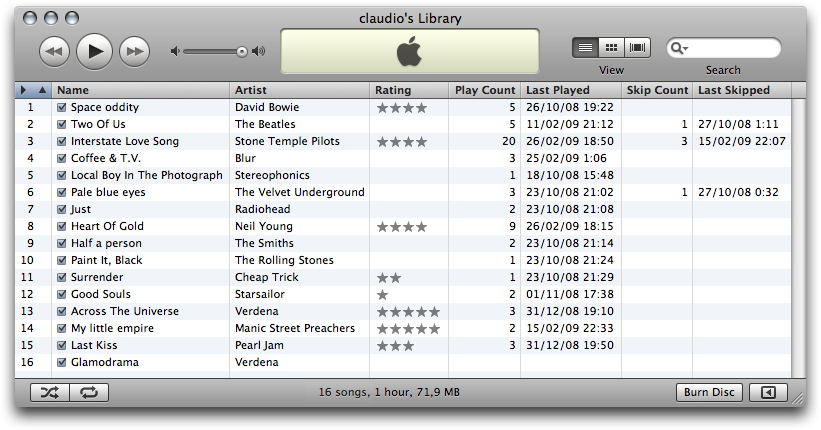
\epsfig{file=img/itunes_claudio, width=\textwidth}
\caption{Personal music library managed with iTunes.}
\label{fig:itunes_claudio}
\end{figure}

Listening behaviour data is very descriptive of personal preferences: 
having played certain songs and not other ones outlines the musical taste of an individual better than a verbal description, with its inaccuracies and misinterpretations, would.

As many persons share their listening behaviour data on the Internet to make their friends aware of their musical habits, the Web has become the best place where to find data about which songs a person has played, when, how they were rated, et cetera.
%For example, the list of songs I have been listening to in the last four years is publicly available in my Last.fm profile page. % LINK

%This chapter presents a technique that, given listening behaviour data of any individual, is able to identify that person's favourite songs and, generically, to \emph{measure how much} that individual shows to like each available song.

The purpose of this chapter is to introduce a measure of \textbf{musical preference} that automatically estimates how much a person likes a given song based on personal listening habits data collected from the Web.

% Sharing this data on the Internet is simple, thanks to tools that automatically connect personal music libraries to the Web, tracking and publishing in real time data about the music played.
% %
% To know which music a person likes is then a matter of finding that person's listening history on the Web and analysing the retrieved data to identify which songs that person prefers.
% 
% The purpose of this chapter is to present a technique to transform listening habits data into a degree of musical preference that measures \emph{how much} each individual shows to like each song.
% 
%The advantage of this technique is that it models musical preferences just observing how music has been \emph{experienced} rather than asking for a verbal description of musical taste.

% Many persons make their listening behaviour data public by sharing them in online communities. This is done through automatic tools that detect songs in personal digital players and publish their usage data on the Web.
% MusicStrands, for instance, provides a software called MyStrands that works both with Apple iTunes and Windows Media Player.
% Similarly, Last.fm provides a tool called Audioscrobbler that tracks all the songs reproduced in digital and portable players (Apple iTunes, Windows Media Player, Winamp, iPod, iPhone, Android) to show them on Last.fm member pages.
% 
% Tracking individual listening behaviour data is very helpful to understand which kind of music a person likes.
% The actual \emph{experience} of selecting a particular set of songs to play from a possibly large music library offers a valuable hint about which music a person likes.
% In my opinion, \emph{observing} what a person plays is more valuable than \emph{asking} about one's musical taste, since verbal descriptions are more subject to inaccuracy and misinterpretation. 
% 
% The goal of this chapter is the following: given a group of people $\mathcal{U}$ and a set of songs $\mathcal{C}$ obtain from the Web experience data about how each member $U \in \mathcal{U}$ has been listening to each song $X \in \mathcal{C}$ and, from this data, measure \emph{how much} each person likes each song in the set.
% 
% The purpose is to show how the musical preferences of each individual can be modelled just with data that describes how a person \emph{used} music in the past, without the need to verbally state which music a person likes best.


 
% Listening behaviour data intrinsically reveals a valuable personal experience.
% The goal of this chapter is to explain how this experience can be analysed in order to estimate the preferences of an individual for a set of songs and artists.
% 
% The purpose of this chapter is to introduce a technique to measure the \textbf{musical preferences} of an individual based on the analysis of listening behaviour data included in personal music library.
% 
% The approach that I propose consists in (1) retrieving personal music libraries from the Internet, and (2) analysing the intrinsic listening behaviour to determine which songs and artists each listener mostly prefers.
% 
% Sect.NN reviews previous works on user modelling, comparing two strategies to build a profile of individual preferences. Sect.NN ..

% section listening_behaviour (end)

\section{Previous work} % (fold)
\label{sec:user_modelling_techniques}

The issue faced in this chapter consists in identifying a set of individual musical preferences without having to explicitly ask for them.
The process of acquiring user preferences is known as user modelling \cite{Rich79,Kass88,Kobsa01} and can either be explicit or implicit.

\subsection{Explicit user modelling} % (fold)
\label{sub:explicit_models}

Explicit acquisition of preferences is obtained when individuals \emph{actively} provide specific facts about loved items.
Most online stores, for instance, ask their users to provide feedback about purchased items: Amazon collects ratings about books, Trip Advisor about travel destinations, eBay about sellers' reputation.

Explicit feedback is the most direct way for users to express their taste, although \citet{Claypool01} noticed how having to stop to enter explicit ratings can alter normal patterns of information usage, and \citet{Zhang02} proved how users can rapidly stop providing explicit ratings unless they perceive a benefit. 
Amazon and eBay, for instance, gratify frequent raters highlighting their profiles as `experts' within the community of users.

 \citet{Potter08} also pointed out how explicit statements require users to `translate' their inner preferences into a score, which is not an immediate and unequivocal process: deciding how many `stars' to assign to a good item is a matter of personal interpretation.
\citet{Banerjee92} also noticed that users asked to rate an item are easily influenced by the scorings assigned by previous users. % \emph{Herding}  refers to the fact that and, as shown in \cite{Cosley03}, this can worsen future recommendations about that item.

% subsection explicit_models (end)

\subsection{Implicit user modelling} % (fold)
\label{sub:implicit_models}

Implicit user modelling % is the alternative approach to explicit preferences described in this chapter and 
takes place by \emph{observing} user actions and inferring preferences from the observed behaviours.
For instance, someone always buying clothes in the same store implicitly expresses a preference for that fashion style. 
Similarly, forwarding an online video to ten friends implicitly demonstrates an interest for that video. %, regardless of any assigned rating.

In different publications, \citet{Nichols97}, \citet{Oard01} and \citet{Kelly03} have categorised several types of actions as possible sources for implicit user modelling.
Figure~\ref{fig:implicit-feedbacks} reports the list of actions according to the underlying purpose of the observed action (Behaviour Category), and to the smallest possible scope of the item being acted upon (Minimum Scope).
In the domain of music, for instance, having either purchased, saved, rated or listened a specific song can be interpreted as an implicit preference for that song.

\begin{figure}[bthp]
\centering \setlength{\abovecaptionskip}{3pt}
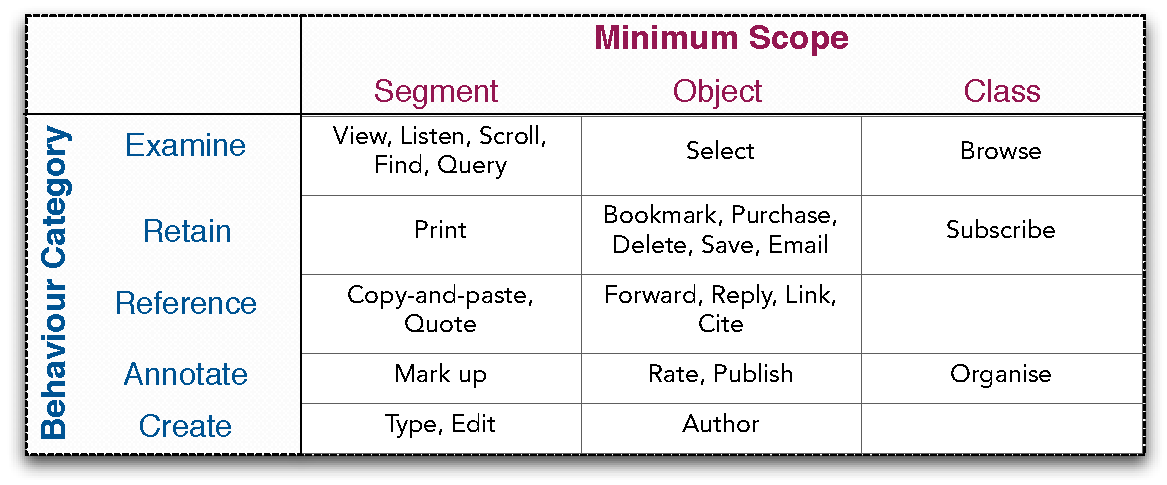
\epsfig{file=img/fig3_2, width=\textwidth}
\caption{Classification of behaviours used to infer implicit feedback.}
\label{fig:implicit-feedbacks}
\end{figure}

% subsection implicit_models (end)

\subsection{Building user profiles} % (fold)
\label{sub:building_user_profiles}

Collecting implicit or explicit preferences is only the first step to compile a comprehensive model of user preferences.
As pointed out by \citet{Hofmann04}, different users associate different meanings with ratings; for instance, `4 out of 5 stars' may have a different meaning for different people. 
For this reason, individual preferences need be \emph{normalised} in order to be compared. 
%\cite{Hu07b} demonstrated how almost all products in Amazon have an asymmetric bimodal (J-shaped) distribution with more positive than negative reviews.
\citet{Goldberg01} proposed to normalise each rating by subtracting its mean rating over all users, and then dividing by its standard deviation.

Another relevant aspect of user modelling is how to build a comprehensive model when only a few individual preferences are available.
\citet{Dieterich93} suggested to either start with an \emph{empty} model, to classify the user into one \emph{stereotypical} category, or to build an initial \emph{individual} model based on a preliminary question-answering session. 
A stereotypical approach, for instance, is used by Last.fm which uses geographical position obtained from the IP address of unregistered users to  recommend musical events taking place in the area where users are located.

Interests may change along time, so a system that learns a model of the user's interests should be based on algorithms that can quickly adjust to changing interests.
The notion of changing target concepts is known as ``concept drift'' \cite{Billsus07}, or ``persistence of interest'' \cite{Lieberman95}.
\citet{Dieterich93} distinguished between ``short-term'' data\,---\,user preferences that are valid only for the current context or session\,---\,and ``long-term'' data\,---\,which should be kept beyond the current session and saved in a permanent storage medium. 
In the domain of music, for instance, Last.fm online radio differentiates between `skipping' a song (short-term negative preference) and `banning' a song (long-term negative preference) from a personalised music channel.

% [Talk about explicit approaches for preferences, like photo Identikit]

% subsection building_user_profiles (end)

% section user_modelling_techniques (end)

%% section problem_description2 (end)
% 
% \section{Explicit approach} % (fold)
% \label{sec:explicit_approach}
% 
% The easiest way to determine how much a person would like to listen to a specific song in a radio channel is through direct feedback.
% Poolcasting Web Radio offers a Web interface that allows anyone to express a personal evaluation about the songs available on a channel (Fig.~\ref{fig:pwr_rate}).
% By clicking on the `Good' and `Bad' buttons , listeners can express their explicit preferences.
% %
% \begin{figure}[bthp]
% \centering \setlength{\abovecaptionskip}{3pt}
% \epsfig{file=img/radio_rate, width=\textwidth}
% \caption{Poolcasting Web Radio allows explicit song rating.}
% \label{fig:pwr_rate}
% \end{figure}
% 
% The \textbf{explicit preference} is denoted as the function $e: \mathcal{U} \times \mathcal{C} \times \mathbb{N}^+ \to [-1,1]$, where a positive (resp., negative) value $e(U,X,T)$ indicates that a participant $U$ would (resp., would not) like a song $X$ to be played on the channel at time $T$, and a value of zero denotes indifference.
% 
% Initially, the explicit preference is null for each listener $U \in \mathcal{U}$ and each song $X \in \mathcal{C}$.
% As participants express their explicit feedback, poolcasting updates these values accordingly.
% To express a slightly positive preference for a song $X$, a participant $U$ clicks \emph{once} the `Good' button, and the explicit preference is updated to $e(U,X,T) = 0.5$. Clicking \emph{twice} or more the `Good' button is interpreted as a strong positive preference, and stored as $e(U,X,T) = 1$.
% Similarly, clicking once on the `Bad' button results in $e(U,X,T) = -0.5$, while clicking twice or more results in $e(U,X,T) = 1$.
% Clicking first on `Good' and then on `Bad' or vice versa resets the value to $e(U,X,T) = 0$.
% 
% %In this way, listeners can express either a very negative, negative, null, positive, or very positive preference for any song by means of two feedback buttons.
% 
% The reason why the explicit preference $e(U,X,T)$ is a function of time $T$ is because participants can change their mind about a song over time; for instance a participant might initially love to hear `Holiday' by Madonna played on a channel and, after a certain time, might not care about `Holiday' being played since another song by Madonna has been broadcast meanwhile.
% 
% The time $T \in \mathbb{N}^+$ represents the number of songs played on the channel so far; when a channel is created $T = 0$, when the first song has been played $T = 1$, and so on. 
% The explicit preference $e(U,X,T)$ corresponds to the most recent statement expressed by the listener $U$ about the song $X$ at time $T$.
% 
% \begin{example}
% A participant $U$ listens to a radio channel broadcasting music from the Eighties.
% After three songs, $U$ wishes song $X$ `Holiday' by Madonna to be played, so $U$ clicks once on `Good', resulting in $e(U,X,3) = 0.5$.
% After two more songs, $U$ wishes song $Y$ `True Colors' by Cyndi Lauper to be played, so $U$ clicks twice on `Good', resulting in $e(U,Y,5) = 1$.
% After three more songs, $U$ becomes indifferent about `Holiday' being played, since another song by Madonna has been broadcast meanwhile, so $U$ clicks once on `Bad', updating the explicit preference to $e(U,X,8) = 0$.
% \end{example}
% 
% Explicit statements are the most direct way for poolcasting to gather individual musical preferences.
% Nevertheless, most radio listeners do not wish to spend a lot of time and effort in evaluating the songs proposed by the radio.
% For this reason, poolcasting integrates this explicit approach with an implicit approach that can estimate the musical taste of each participant without requiring any interaction.
% % section explicit_approach (end)
% 
\section{Gathering listening habits} % (fold)
\label{sec:implicit_approach}

To determine individual music preferences from the analysis of personal listening habits, these have to be collected first, which can occur in two ways.

The first method is to extract this information directly from personal music libraries. 
Apple iTunes, for instance, stores in the hard disk a file called `iTunes Library.xml' which describes the list of played songs, play counts, play recency, skip counts, user ratings.
Parsing this XML file provides first-hand knowledge about the music played on that particular machine.

The second method is to gather this knowledge from the Internet.
Different tools track personal listening habits and make these data available on the Web.
Last.fm, for instance, provides each member with a Web page showing the last songs played, the device where they were played and the assigned rating, as detected by the music tracking software Audioscrobbler (see Fig.~\ref{fig:lastfmprofile}).
MusicStrands offers a similar service with a tool called MyStrands (see Fig.~\ref{fig:musicstrands}).
%
\begin{figure}[bthp]
\centering \setlength{\abovecaptionskip}{3pt}
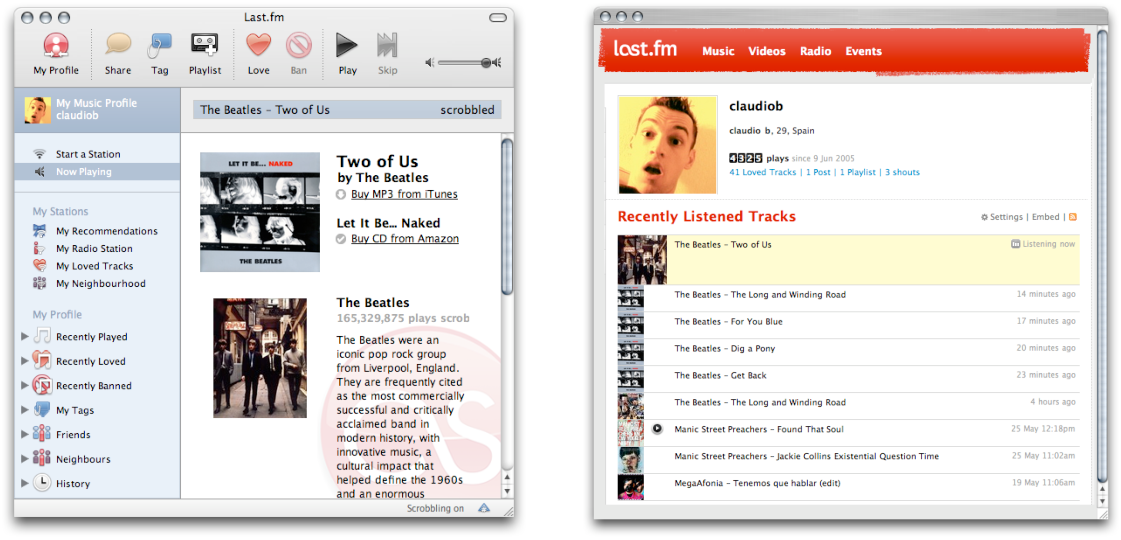
\epsfig{file=img/lastfm, width=\textwidth}
\caption{Last.fm tracking tool Audioscrobbler and profile Web page.}
\label{fig:lastfmprofile}
\end{figure}
%
\begin{figure}[bthp]
\centering \setlength{\abovecaptionskip}{3pt}
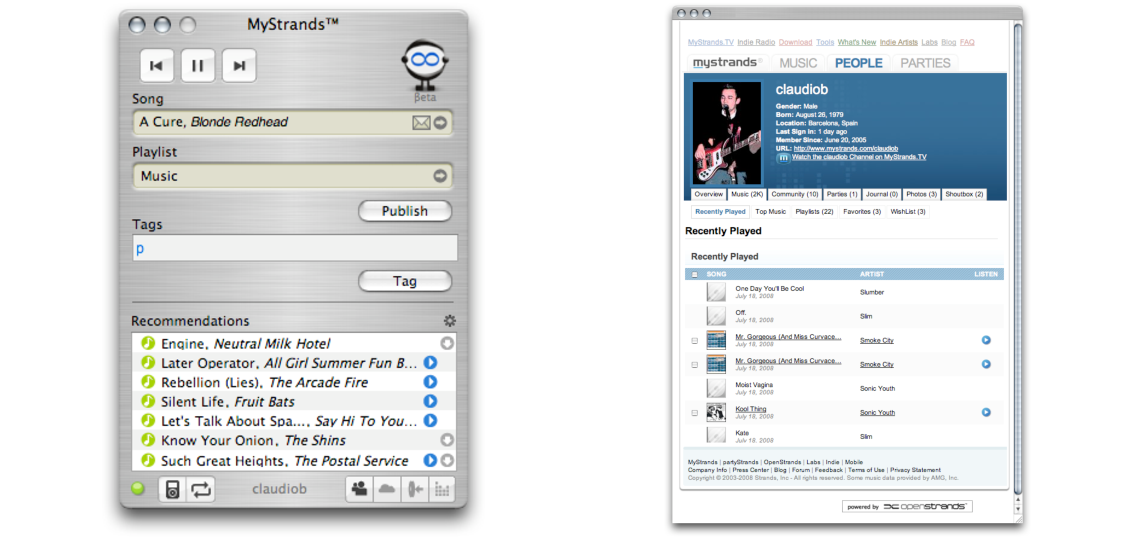
\epsfig{file=img/musicstrands, width=\textwidth}
\caption{MusicStrands tracking tool MyStrands and profile Web page.}
\label{fig:musicstrands}
\end{figure}

Gathering listening habits from the Web has four main advantages.
Firstly, data can be collected from thousands of users without having to access their hard disks.
Secondly, Web services provide Web Application Programming Interfaces (API) \cite{Booth04} to rapidly retrieve large amount of data in a standard XML format.
Thirdly, Web services can automatically fix mistakes in song titles (e.g., `Obladi Oblada' rather than `Ob-la-di Ob-la-da') thus correctly identifying played songs.
Fourthly, Web services can automatically aggregate the listening habits from multiple devices; for instance Last.fm `scrobbles' both songs played in portable devices (iPod, iPhone, Android) and digital libraries (iTunes, Windows Media Player, Winamp).


%The next section will explain how the play count and rating of each song can effectively be combined to estimate the degree in which a person likes that song.

% There are several Web communities that allow people to share their listening behaviours online, and most of them provide tools to rapidly gather this knowledge for different users.
% Last.fm, for instance, provides a Web API [CITE] that gives direct access to the list of songs played by any member of Last.fm in a tracked device.
% Similarly, MusicStrands offers the OpenStrands API to access individual listening behaviour data.
% 
% The granularity of information stored by these communities is not uniform. Last.fm, for instance, reports when each member played each song, on which device, and whether the song was rated or skipped; OpenStrands reports only about played songs and ratings.
% 
% Of all the listening behaviour data that can be collected online about a person, there are two properties that most clearly identify which music a person most likes: \textbf{user ratings} and \textbf{play counts}. 
% The simple fact that a song has been (1) rated positively and (2) played many times denote an interest of the listener for that song.
% Other properties are more subject to noise; for example the fact of \emph{skipping} a playing song is not necessarily related to the preference for that song, that song might just not fit well in the current musical context.
% 
% In brief, the Web contains a lot of experience data about which songs were played by different persons. Given a person $U \in mathcal{U}$ and a song $X \in \mathcal{C}$, information can be extracted regarding how $U$ rated song $X$ and how many times $U$ listened to $X$. 
% This information can be used to estimate the degree in which $U$ shows to prefer song $X$, as will be presented in the following section.
% 

\section{Estimating individual preferences} % (fold)
\label{sec:estimating_individual_preferences}

Once listening habits data have been collected, a choice has to be made about which part of these data can be considered as illustrative of music preferences.

One relevant property is clearly the \textbf{user rating} assigned to each song. 
Almost every digital player enables listener to vote for favourite songs; Apple iTunes uses `stars' (from 1 to 5), while Audioscrobbler gives the option to mark a song as either `Loved' or `Banned'.

A second relevant property is the \textbf{play count}: how many times a song was played. Intuitively, the interest of a person for a song is directly related to its play count, especially if the song has been played often recently.

Other relevant properties, such as the skip count and the play recency, will not be utilised since they are more subject to interpretation. % than user rating and play count. 
Skipping a song, for instance, might be interpreted as a negative preference, but listeners also skip songs they like when these do not fit in the current context. 

The rest of this section explains how, given the ratings assigned by a person to a set of  songs and their play counts, a measure of \textbf{individual preference} for each song can be defined.

\subsection{Usage behaviour normalisation} % (fold)
\label{sub:usage_behaviour_normalisation}

Let $\mathcal{U}$ be a group of people and let $U \in \mathcal{U}$ be a person for which listening habits data are available with respect to a set of songs  $\mathcal{C}$.
Let $r: \mathcal{U} \times \mathcal{C} \to [\varrho_{\min}, \varrho_{\max}]$ be the rating assigned by $U$ to each song, where $\varrho_{\min}$ and $\varrho_{\max}$ are the minimum and maximum rating scores (e.g., $\varrho_{\min} = 1$ and $\varrho_{\max} = 5$ `stars' in Apple iTunes), and
let $n: \mathcal{U} \times \mathcal{C} \to \mathbb{N}$ be the play count, that is, the number of times that $U$ played each song.

The goal is to combine for each song $X \in \mathcal{C}$ the two values $r(U,X)$ and $n(U,X)$ in order to measure the \textbf{individual preference} degree $i: \mathcal{U} \times \mathcal{C} \to [0,1]$, that is, how much $U$ shows to like song $X$.

High ratings and high play counts identify songs a listener likes. 
The `absolute' values of rating and play count, though, offer small information to estimate a preference degree.
%
Having listened to a song 3 times or having assigned a rating of `3 out of 5' stars, for instance, do not clearly indicate whether a listener likes a song or not. If that listener normally rates songs with only 1 or 2 stars, then giving 3 stars expresses a positive preference. 
If the average rating is instead 4 or 5 stars, then 3 stars is probably not a good signal.
Similarly, a play count of 3 is significant or not whether the listener is a sporadic or a frequent music listener.

User ratings and play counts are values that are relevant only with respect to the \emph{average listening behaviour}.
Only songs showing a play count or a rating above the average can significantly be considered as favourite songs.
For this reason, user ratings $r(U,X)$ and play counts $n(U,X)$ are hereafter \emph{normalised} to yield values in the range $[-1,1]$, so that only songs `above the average' are assigned positive values.


\subsection{Normalising user rating} % (fold)
\label{sub:normalising_user_rating}


To define a \emph{normalised user rating} means to find a function  $\widehat{r}: \mathcal{U} \times \mathcal{C} \to [-1,1]$ which returns positive (resp., negative, null) values for songs rated higher than (resp., lower than, equal to) the average. 
Let $\mathcal{R}_U \subseteq \mathcal{C}$ be the songs that a person $U \in \mathcal{U}$ has ever rated and let
%
\begin{equation*}
   \overline{r(U)} = \frac{\sum_{X \in \mathcal{R}_U} r(U,X)}{\#(\mathcal{R}_U)}       
\end{equation*}
be the average user rating of $U$.
The normalised user rating $\widehat{r}(U,X)$ is a function that satisfies these conditions:
\begin{equation}\label{eq:normalisation_conditions_1}
\left\{ \begin{array}{lll}
\rule[-1em]{0pt}{2.5em}
r(U,X) < \overline{r(U)} & \implies & -1 < \widehat{r}(U,X) < 0 \\
\rule[-1em]{0pt}{2.5em}  
r(U,X) = \overline{r(U)} & \implies & \widehat{r}(U,X) = 0 \\
\rule[-1em]{0pt}{2.5em}  
\overline{r(U)} < r(U,X) & \implies & 0 < \widehat{r}(U,X) < 1
\end{array} \right.
\end{equation}
and such that any song with the lowest (resp., highest) possible rating obtains the minimum (resp., maximum) possible normalised value:
\begin{equation}\label{eq:normalisation_conditions_2}
\left\{ \begin{array}{lll}
\rule[-1em]{0pt}{2.5em}
r(U,X) = \varrho_{\min}  & \implies & \widehat{r}(U,X) = -1 \\ 
%\rule[-1em]{0pt}{2.5em}  
%r(U,X) = \overline{r(U)} & \implies & \widehat{r}(U,X) = 0 \\
\rule[-1em]{0pt}{2.5em}  
r(U,X) = \varrho_{\max} & \implies & \widehat{r}(U,X) = 1%\,,
\end{array} \right.
\end{equation}
under the condition that $\varrho_{\min} < \overline{r(U)} < \varrho_{\max}$.

% Formally, I indicate with $i: \mathcal{U} \times \mathcal{C} \to [0,1]$ the \textbf{implicit preference} inferred by poolcasting from usage behaviour [ ONLY FROM $o$, right?], where $i(U,X)$ refers to how much a participant $U$ shows to like an item $X$: the higher the value, the more $U$ shows to like $X$. %, a value of 0 denotes indifference.
% 
% Formally, let 
% then $U$ implicitly likes every song $X \in \mathcal{L}_U$ used more than the average:
% \begin{equation}\label{eq:infer_implicit}
% \left\{ \begin{array}{lll}
% 	\rule[-1em]{0pt}{2.5em}  
% 	r(U,X) \leqslant \overline{r(U)} & \implies & i(U,X) = 0\\
% 	\rule[-1em]{0pt}{2.5em}  
% 	r(U,X) > \overline{r(U)} & \implies & i(U,X) > 0\,.\\
% \end{array} \right.
% \end{equation}
% 
% 
% Let $\widehat{r}: \mathcal{U} \times \mathcal{C} \to [-1,1]$ be the normalised version of the observed usage property $o$.
% Items showing a usage property higher than (respectively, lower than) the average are assigned a positive (resp., negative) normalised value:
% 
% Items showing exactly an average usage property are assigned a normalised value of $0$; other items are assigned a normalised value of $-1$ (respectively, $1$) only if they show the lowest (resp., highest) possible usage property values:
% where:

One function that fulfils \eqref{eq:normalisation_conditions_1} and \eqref{eq:normalisation_conditions_2} and is furthermore continuous, monotonic, derivable, with the first derivative monotonic in the interval $(-1,1)$ is the function that solves the following linear equation system:
\begin{equation*}%\label{eq:linear_system}
\left\{ \begin{array}{ll}
\rule[-1em]{0pt}{2.5em}
a\log(b + \varrho_{\min}) + c = -1\\
\rule[-1em]{0pt}{2.5em}
a\log(b + \overline{r(U)}) + c = 0\\
\rule[-1em]{0pt}{2.5em}
a\log(b + \varrho_{\max}) + c = 1
\end{array} \right.
\end{equation*}
and that yields $0$ when $r(U,X) = \overline{r(U)}$.
The solution of this system is defined by cases:
\begin{equation*}
\widehat{r}(U,X) = 
\begin{cases}
%\rule[-1em]{0pt}{2em} 
%-1 
%& \text{if $\overline{r(U)} = \varrho_{\min}$}\\        
\rule[-1em]{0pt}{2em} 
0 
&\hspace{-2em}\text{if $r(U,X) = \overline{r(U)}$}\\   
\rule[-1em]{0pt}{3em} 
\cfrac{2(r(U,X) - {\varrho_{\med}}^2)}{\varrho_{\max} -\varrho_{\min}} 
&\hspace{-1em}\text{if $\overline{r(U)} = \varrho_{\med}$}\\
\rule[-1em]{0pt}{6em} 
\cfrac{\log\cfrac{2r(U,X)(\varrho_{\med} - \overline{r(U)}) + \overline{r(U)}^2 - \varrho_{\max}\varrho_{\min}}{(\varrho_{\max} - \overline{r(U)})(\overline{r(U)} - \varrho_{\min})}}
 {\log(\varrho_{\max} - \overline{r(U)}) - \log(\overline{r(U)} -  \varrho_{\min})} 
& \text{otherwise,}
\end{cases}
\end{equation*}
where $\varrho_{\med} = \frac{1}{2}(\varrho_{\min} + \varrho_{\max})$. % (e.g., 3 stars in iTunes). % is the median possible value for the property.
%


The three cases defining $\widehat{r}(U,X)$ are separately illustrated in Fig.~\ref{fig:normalisation_function} and depend on the average rating $\overline{r(U)}$ of each person $U$:
\begin{itemize}
 \item when $U$ assigns the same rating to every song, then 
$r(U,X) = \overline{r(U)}$ for every song and $\widehat{r}(U,X)$ falls back to the constant $0$ (solid line in Fig.~\ref{fig:normalisation_function});
% \item when $U$ has the maximum usage behaviour possible for every item, then $\overline{r(U)} = \varrho_{\max}$ and $\widehat{r}(U,X)$ falls back to the constant $1$ (higher dotted line in Fig.~\ref{fig:normalisation_function});
 \item when $U$ has an average rating of $\varrho_{\med}$, then $\widehat{r}(U,X)$ falls back to a linear function (dashed line in Fig.~\ref{fig:normalisation_function}); % with zero-cross in $X = \varrho_{\med}$; 
 \item otherwise $\widehat{r}(U,X)$ is a logarithmic function, concave or convex whether the average rating $\overline{r(U)}$ is higher or lower than $\varrho_{\med}$ (dotted lines in Fig.~\ref{fig:normalisation_function}). 
\end{itemize}
%
\begin{figure}[bthp]
\centering \setlength{\abovecaptionskip}{3pt}
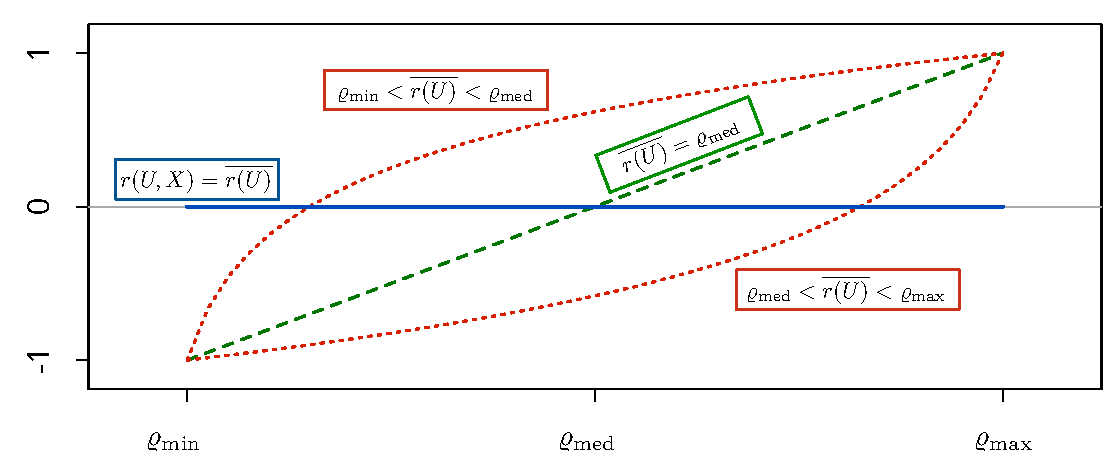
\epsfig{file=img/fig3_5, width=\textwidth}
\caption{Normalised user ratings corresponding to different values of $\overline{r(U)}$.}
\label{fig:normalisation_function}
\end{figure}
Working with normalised values, every rating is interpreted with respect to each user, and the same absolute rating (e.g., 4 stars) can assume different normalised values $\widehat{r}(U,X)$ for different people.

\begin{example}
Figure~\ref{fig:compared_normalisation} represents the situation where two friends $U$ and $V$ have both listened to ten songs $\mathcal{C} = \{X1, X2, \ldots, X10\}$ and have rated them with different criteria.
Even though $U$ and $V$ both assigned four stars to song $X5$, the normalised user rating for this song differs: $\widehat{r}(U,X5) = 0.67$ is positive, while $\widehat{r}(V,X5) = 0$ is not.
The reason is that $U$ assigns in average two stars to each song, so the observed value $r(U,X5) = 4$, higher than the average, corresponds to a positive normalised user rating, while $V$ assigns in average four stars to every song, so the observed value $r(V,X5) = 4$ is not equally significant.
%
\begin{figure}[bthp]
\centering \setlength{\abovecaptionskip}{3pt}
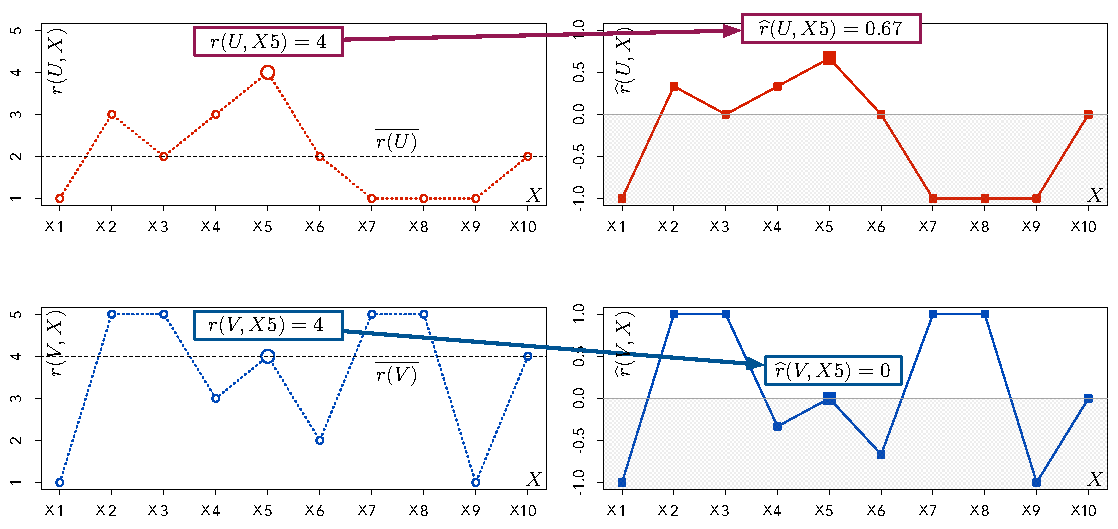
\epsfig{file=img/fig3_6, width=\textwidth}
\caption{Effect of the normalisation process on user ratings.}
%xample of two participants $X$ and $Y$ showing equal behaviour $o$ for the same item $X5$ but having different normalised values $\widehat{r}$.} 
\label{fig:compared_normalisation}
\end{figure}
        
\end{example}

% subsection usage_behaviour_normalisation (end)

\subsection{Combining user ratings and play counts} % (fold)
\label{sub:positive_and_negative_implicit_preferences}

Following the same approach described to normalise user ratings, play counts $n(U,X)$ can be normalised as well, resulting in a normalised play count function $\widehat{n}: \mathcal{U} \times \mathcal{C} \to [-1,1]$ that yields positive (resp., negative, null) values for songs played more than (resp., less than, as much as) the average play count.

Normalising user ratings and play counts helps identify songs for which a person has a particular interest: 
every song $X$ for which $\widehat{r}(U,X) > 0$ or $\widehat{n}(U,X) > 0$ has obtained by $U$ a rating or play count higher than the average and, as such, can be assessed as one of the songs preferred by $U$.

Formally, the \textbf{individual preference} degree $i: \mathcal{U} \times \mathcal{C} \to [0,1]$ that measures how much $U$ likes each song $X \in \mathcal{C}$ is defined as a linear combination of these normalised properties:
\begin{equation}\label{eq:implicit_preference}
i(U,X) = \pi \cdot \max(0,\widehat{r}(U,X)) + (1 - \pi) \cdot \max(0,\widehat{n}(U,X)) % \max(0,\widehat{o_J}(U,X))
\end{equation}
where $\pi \in [0,1]$ denotes the importance assigned to ratings with respect to play counts.

The reason why both normalised rating and play count are limited to a minimum value of zero is that implicit preferences are assessed only for songs for which either the rating or the play count is above the average.
No `negative' assumption is made about songs rated or played less than average.
The reason is that a person may have not rated or played a specific song for several reasons (lack of time, of a digital player, of the right occasion) and this should not be always interpreted as a lack of interest.
On the other hand, having taken the effort to rate or play often a song should be positively interpreted as an implicit measure of interest.

This technique allows to estimate individual music preferences without any explicit action by the listener, exploiting only knowledge implicit in the listening habits data of a person.

\begin{example}
The music library shown in Fig.~\ref{fig:itunes_claudio} contains 8 rated songs, with an average rating of 3.5 stars; five songs were rated above this value.
Similarly, 15 songs have been played, the average play count is 4 and four songs have a play count above this value.
The implicit preference of the author for these songs can be calculated with the function \eqref{eq:implicit_preference} assigning the same importance to ratings and play counts ($\pi = 0.5$).
The results are reported in Table~\ref{table:itunes}:
`Interstate Love Song' (Stone Temple Pilots) stands out as the author's favourite song, followed by `Across The Universe' (Verdena) and `My Little Empire' (Manic Street Preachers). 
A song such as `Last Kiss' (Pearl Jam) is not in the list because both its rating (3 stars) and its play count (3) fall below the average.
\end{example}

%\vspace{0.3cm}
\begin{table}[bhtp]
\centering \setlength{\abovecaptionskip}{3pt}
\caption{Individual preferences assessed for songs in Fig.~\ref{fig:itunes_claudio}.}\label{table:itunes}
\begin{tabular}{|cc|c|c|c|c|c|}
\hline
\multicolumn{2}{|c|}{song}&\multicolumn{2}{c|}{rating}&\multicolumn{2}{c|}{play count}&preference\\
\multicolumn{2}{|c|}{$X$}&$r(U,X)$&$\widehat{r}(U,X)$&$n(U,X)$&$\widehat{n}(U,X)$&$i(U,X)$\\
\hline

\multirow{2}{*}{3}  & \small{Interstate} & \multirow{2}{*}{4} & 
\multirow{2}{*}{0.28} & \multirow{2}{*}{20} & \multirow{2}{*}{1} & \multirow{2}{*}{\textbf{0.64}}\\ & \small{Love Song} &&&&& \\ \hline

\multirow{2}{*}{13}  & \small{Across The} & \multirow{2}{*}{5} & 
\multirow{2}{*}{1} & \multirow{2}{*}{3} & \multirow{2}{*}{0} & 
\multirow{2}{*}{\textbf{0.50}}\\ & \small{Universe} &&&&& \\ \hline

\multirow{2}{*}{14}  & \small{My Little} & \multirow{2}{*}{5} & 
\multirow{2}{*}{1} & \multirow{2}{*}{2} & \multirow{2}{*}{0} &
\multirow{2}{*}{\textbf{0.50}}\\ & \small{Empire} &&&&& \\ \hline

\multirow{2}{*}{8}  & \small{Heart} & \multirow{2}{*}{4} & 
\multirow{2}{*}{0.28} & \multirow{2}{*}{9} & \multirow{2}{*}{0.5} & 
\multirow{2}{*}{\textbf{0.39}}\\ & \small{Of Gold} &&&&& \\ \hline

\multirow{2}{*}{1}  & \small{Space} & \multirow{2}{*}{4} & \multirow{2}{*}{0.28} & \multirow{2}{*}{5} & \multirow{2}{*}{0.12} & \multirow{2}{*}{\textbf{0.20}}\\ & \small{Oddity} &&&&& \\ \hline

\multirow{2}{*}{2}  & \small{Two} & \multirow{2}{*}{---} & 
\multirow{2}{*}{---} & \multirow{2}{*}{5} & \multirow{2}{*}{0.12} & \multirow{2}{*}{\textbf{0.12}}\\ & \small{Of Us} &&&&& \\ \hline


\end{tabular}
\end{table}
%\vspace{0.3cm}



% 
% The normalised function $\widehat{r}(U,X)$ represents how a person $U$ rated a song $X$ with respect to the average individual rating.
% If $U$ has assigned to $X$ a rating higher than the average, then $\widehat{r}(U,X)$ is positive, and a positive implicit preference can be assessed for $X$.
% If $U$ has assigned to $X$ a rating lower than the average, then no assumption should be done about implicit preferences.
% Therefore the implicit preference of a user $U$ for a song $X \in \mathcal{L}_U$ can be estimated from the user rating $r(U,X)$ as the function:
% \begin{equation}\label{eq:implicit_one}
% 	\max(0, \widehat{r}(U,X))\,.
% \end{equation}
% which returns positive values for songs rated more than the average, and returns 0 for songs rated equal or less than the average.
% 
% % According to \eqref{eq:infer_implicit}, poolcasting infers a positive implicit preference in this case. 
% % %Poolcasting uses this value to quantify the implicit preference for each item $X \in \mathcal{L}_U$.
% % Given one observable property $r(U,X)$, poolcasting estimates the implicit preference of participant $U$ for an item $X$ as:
% % \begin{equation*}
% % \begin{cases}
% % \rule[-1em]{0pt}{2em} 
% % i(U,X) = \widehat{r}(U,X) & \text{if $\widehat{r}(U,X) > 0$}\\        
% % \rule[-1em]{0pt}{2em} 
% % i(U,X) = 0 & \text{otherwise.}
% % \end{cases}
% % \end{equation*}
% % This formula can be written in a more compact style as:
% 
% % subsection positive_and_negative_implicit_preferences (end)
% 
% \subsection{Inferring implicit preference from multiple usage properties} % (fold)
% \label{sub:combining_multiple_observable_properties}
% 
% Star rating is just one of the way people express their listening behaviours.
% As shown in Fig.~\ref{fig:itunes_claudio}, digital libraries store more usage behaviour data than just user ratings.
% By combining many of these properties, a more comprehensive degree of implicit preference can be obtained.
% For instance, an implicit preference can be assessed for any song rated more than 3 stars, listened at least twice and skipped no more than 4 times.
% 
% 
% %Participants might show more than one observable usage behaviour property at the same time; for instance poolcasting might know \emph{both} the number of times a person listened to a song \emph{and} how many friends that song was recommended to. In this case, poolcasting infers implicit preference through a linear combination of normalised behaviour values.
% 
% Let $N$ be the number of observable properties of a participant $U$ for an item $X \in \mathcal{L}_U$ (e.g., user rating, play count), let $o_1, o_2, \ldots, o_N$ be their absolute values, and let $\widehat{o_1}, \widehat{o_2}, \ldots, \widehat{o_N}$ be their respective normalised values.
% The function $i: \mathcal{U} \times \mathcal{C} \to [0,1]$ that estimates the \textbf{implicit preference} of a participant $U$ for a song $X$ based on all the observed properties is defined as:
% \begin{equation}\label{eq:implicit_preference}
% i(U,X) = \sum_{J=1}^N \pi_J \cdot \max(0,\widehat{o_J}(U,X)) % \max(0,\widehat{o_J}(U,X))
% \end{equation}
% where the parameters $\pi_J \in [0,1]$ denote the importance assigned to each observable property, under the constraint that $\sum_{J=1}^N \pi_J = 1$.

% subsection combining_multiple_observable_properties (end)


% \section{The application} % (fold)
% \label{sec:the_application}
% 
% [Here explain a minimum of iTunes format and an example with my own library, with my average usage etc.] 
% More evaluation and tuning of parameters available in Chap7.
% 
% For instance if I combine rating and play count in the iTunes library before I get these values..
% 
% % section the_application (end)

% ction{Explicit statements} % (fold)
% bel{sec:explicit_statements}
% 
% ITHER THIS GOES HERE OR AT THE BEGINNING ]
% 
%  method presented so far allows to infer preferences without asking the individuals. However these preferences are only positive, while a user might want so explicitly state that a song is not appreciated.
% o, these preferences are static, calculated only once, while a user might want to update and change them.
% o these preferences are generic, not specific to a channel. In particular, if iTunes library is analysed, then implicit preferences only about songs you like at work, at home, etc., can be assessed.
% 
% 
%  all these reasons, explicit statements are also permitted...
% 
% 
% ection explicit_statements (end)
%


% subsection contributions5 (end)

\subsection{Integrating additional properties} % (fold)
\label{sub:expanding_to_artists3}

The individual preference degree \eqref{eq:implicit_preference} combines only two observable properties: user ratings and play counts.
Other observable properties can be easily integrated in the function if they are found to be significantly related to musical preferences.
%
The skip count (number of times a song was skipped before its end), for instance, can be considered as an indicator of `negative' preferences.
This property can be included into \eqref{eq:implicit_preference} by first normalising its values to the range $[-1,1]$, then adding this value to the linear combination \eqref{eq:implicit_preference} that defines the value of $i(U,X)$.
The only precaution is to invert negative preferences: songs skipped \emph{less} than the average would yield a positive normalised value and vice versa.

\subsection{Extending to artists} % (fold)
\label{sub:expanding_to_artists2}

Whatever the number of properties considered, songs that have never been `experienced' (played, rated, skipped) are always assigned a value of $i(U,X) = 0$, which means that no implicit preference can be assessed.

This is an intrinsic limitation of the proposed technique: preferences can only be inferred for songs in the individual listening history.
This behaviour can be improved considering that, in general terms, a person has similar preferences for songs by the same artist.
For instance, if $U$ has assigned 5 stars to ten songs by Bj\"{o}rk, then $U$ will probably like future released by Bj\"{o}rk as well, since $U$ shows to enjoy her music. 
In other words, a positive implicit preference for $U$ can be assessed for \emph{any} song by Bj\"{o}rk, even those that $U$ has not yet heard.

Formally, let $X$ be a song that a person $U$ has not yet experienced, and let $\mathcal{Y}_U(X)$ be other songs by the same artist of $X$ that $U$ has experienced:
\begin{equation}
   \mathcal{Y}_U(X) = \{Y\,|\,a(X) = a(Y)\,\wedge\,i(U,X) = 0\}\,.
\end{equation}
Then, the individual preference of $U$ for song $X$ can be estimated as the average preference for known songs by the same artist:
%
\begin{equation*}
        i(U,X) = \sum_{Y \in \mathcal{Y}_U(X)} \frac{i(U,Y)}{\#(\mathcal{Y}_U(X))}\,.
\end{equation*}
%
This extension enables the definition of a degree of implicit preferences also for songs outside of a personal music library.

% subsection expanding_to_artists2 (end)

\section{Summary} % (fold)
\label{sec:contributions5}

This chapter has presented a technique to build individual music profiles from the analysis of personal listening habits.
%
Listening habits describe which songs a person has been listening to and can either be extracted from personal music libraries or collected from Web communities (Last.fm, MusicStrands). % that make them publicly available.

Of all the songs that a person has been playing, the preferred ones are those that have been played more often and have been best rated.
This chapter has presented a technique to automatically measure how much a person likes each listened song.
%
The proposed method analyses the play counts and ratings assigned by any person $U$ to any song $X$ and delivers a measure $i(U,X) \in [-1,1]$ of musical preference.

The technique presented in this chapter will be employed in the poolcasting approach introduced in Chap.~\ref{cha:poolcasting_web_radio} to identify which songs satisfy most of the preferences of a given audience.


%Clearly this method works well for people that (1) listen to music with a digital player (2) are open to make this data available to other and (3) listen to a lot of music or use a lot the rating feature in their player. 

% section contributions5 (end)

% chapter preferences (end)

\chapter{The poolcasting technique} % (fold)
\label{cha:poolcasting_web_radio}
\songquote{With this method that I have found\\
I'm redressing all I know}{Mansun, 1998} 
% Life is a compromise anyway

\section{Adapting music for a group of listeners} % (fold)
\label{sec:adapting_music_for_a_group_of_listeners}

% section adapting_music_for_a_group_of_listeners (end)
The first part of the thesis has explained how to use experience data from the Web to perform two specific tasks: estimate musical association between songs %from a set of playlists 
(Chap.~\ref{cha:smoothness}) and estimate individual music preferences % from listening habits 
(Chap.~\ref{cha:preferences}).

Musical associations (which songs or artists sound well together in sequence) and individual preferences (what the public would like to hear) serve as the basis for the technique described in this chapter, which represents the main contribution of this dissertation.
This technique helps identify, in a large repository of music, a subset of songs adapt for a group of listeners.

While disc jockeys (DJs) can use their senses to perceive the taste of the audience (watching their reaction, listening to their requests) and know from experience which songs mix well one after the other, here the methods introduced in the first part of the thesis % to identify musically associated songs and individual music preferences 
are used to deliver group-customised music sequences (see Fig.~\ref{fig:schema}).
%
\begin{figure}[bthp]
\centering \setlength{\abovecaptionskip}{3pt}
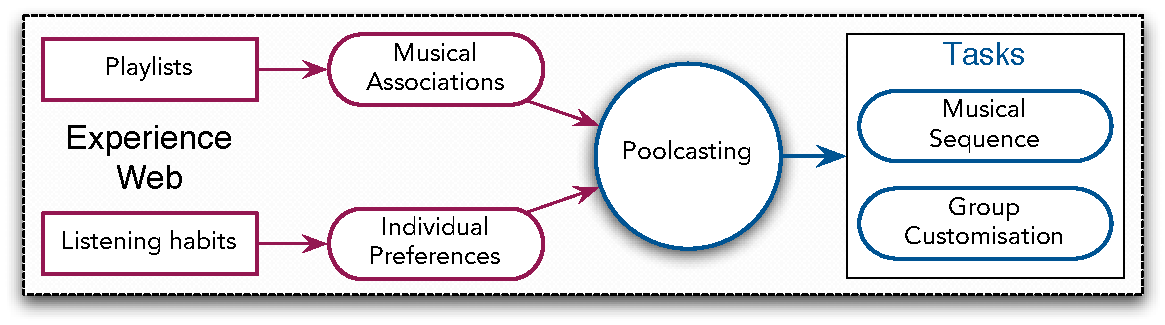
\epsfig{file=img/fig4_1, width=\textwidth}
\caption{Collecting music experiences from the Web to deliver sequences of songs customised for groups of listeners.}
\label{fig:schema}
\end{figure}

\subsection{Problem Definition} % (fold)
\label{sub:problem_definition2}

There are several situations where groups gather to listen to music, such as home parties, discos and, in a virtual sense, radio stations.
In these contexts, someone is entitled to decide \emph{which} songs to play; this can either be a professional DJ or someone from the audience.

%The goal of this chapter is to present a family of techniques called poolcasting that `behave like a good DJ', selecting from a possibly large repository of music a subset of songs that best satisfy the current audience.

In discos and AM/FM radios, expert DJs are appointed to select the best music for the audience. 
In home-parties, bars and online radios, this task is instead typically left in the hands of an automated system, for instance a portable music device (Apple iPod) with the `shuffle' option turned on.

The problem with \textbf{automated music selection} is that the preferences and reactions of the audience are not considered, so the result can be unsatisfactory for the actual listeners. Moreover, an automated selection does not ensure that each played song `sounds well' after the previous one.

The problem addressed in this chapter is whether an intelligent technique can `act as a good DJ', autonomously adapting the music to the listening audience.
Precisely, the goal is to automatically select and deliver a musical sequence that matches four requirements:
 
{\setlength{\leftmargini}{42pt} 
\begin{enumerate}
\renewcommand{\theenumi}{Goal \arabic{enumi}}
%\item\label{p:variety} \textbf{Variety}: the same song or songs by the same artist should be not played multiple times at close distances;
%\item\label{p:smoothness} \textbf{Smoothness}: each song should form a smooth musical transition with the previously played song;
%\item\label{p:customisation} \textbf{Customisation}: each song should match the music preferences of the current listeners; and
%\item\label{p:fairness} \textbf{Fairness}: the whole musical sequence should ensure, in the long run, an equal degree of satisfaction to all the listeners.
\item\label{p:variety} \textbf{Variety}: no song or artist should be repeated within a short period of time;
\item\label{p:smoothness} \textbf{Smoothness}: songs should follow a sequence perceived as musically smooth;
\item\label{p:customisation} \textbf{Customisation}: songs should match the musical interests of the current audience; and
\item\label{p:fairness} \textbf{Fairness}: in the long run, every listener should have a similar degree of satisfaction with respect to the music played.
\end{enumerate}
}
The first two properties are meant to build a good sequence of songs, avoiding repetitions (\ref{p:variety}) and ensuring a certain musical continuity (\ref{p:smoothness}).
The last two properties are meant to customise the music for the group: selecting songs according to the musical taste of the audience (\ref{p:customisation}) and embracing the preferences of every listener in the long run (\ref{p:fairness}).

% subsection problem_definition2 (end)

\subsection{The poolcasting approach} % (fold)
\label{sub:what_is_poolcasting}

This chapter presents poolcasting, an intelligent technique that addresses the music selection problem described above.
Poolcasting generates musical sequences in real time, selecting at each moment which songs to play next based on the current audience and on the set of available songs.



The way in which the four goals of of variety, smoothness, customisation and fairness are addressed is by means of a Case-Based Reasoning (CBR) process that identifies which song to play at each moment.

CBR systems, given a new problem to solve, first \emph{retrieve} similar past problems, then \emph{reuse} their solutions to generate a good solution for the new problem, finally \emph{revise} the proposed solution.
Similarly poolcasting, to select at a given moment which song to play on a channel:
\begin{enumerate}
 \item \emph{(Retrieve Process)} first retrieves a subset of available songs (the retrieved set) that have not been played recently (\ref{p:variety}) and form a smooth musical transition with the last song played (\ref{p:smoothness});
 \item \emph{(Reuse Process)} then ranks the retrieved set according to the preferences of the current audience (\ref{p:customisation}) giving more importance to those listeners less satisfied with the music recently played (\ref{p:fairness}); and  
% \item \emph{(Reuse Process)} then ranks the retrieved set according to the preferences of the current audience (\ref{p:customisation}), identifies in this ranking a song that will keep all the listeners similarly satisfied (\ref{p:fairness}) and selects that song to play next;
 \item \emph{(Revise Process)} finally considers the listeners' feedback to adjust individual preferences % and musical associations 
over time.
\end{enumerate}

In order to know which songs form smooth musical transitions, poolcasting integrates the co-occurrence analysis process introduced in Chap.~\ref{cha:smoothness}. In order to know the preferences of the current audience, poolcasting integrates the implicit user modelling approach described in Chap.~\ref{cha:preferences}. 

% As a result, poolcasting can create musical sequences customised for the listening audience, that achieve the four required goals of variety, smoothness, customisation and fairness.

The rest of the chapter is organised as follows.
Section~\ref{sec:previous_works4} reviews previous work related to Case-Based Reasoning, group-adaptive systems and social choice problems.
%
The CBR process that combines experience knowledge from the Web to customise music for an audience is presented in Sect.~\ref{sec:the_case_based_reasoning_selection_process}.
%
Section~\ref{sec:social-choice-problem} explains how poolcasting can fairly satisfy the entire audience when listeners have different musical tastes.

%Section~\ref{sec:what_i_have_done} describes a Web application providing an online radio service where the poolcasting techniques are employed. This Web radio offers interactive features and social component that stand ahead of existing online radio services.


% The approach of poolcasting to possibly satisfy the \emph{whole} audience is described in Sect.~\ref{sec:social-choice-problem} and consists in achieving fairness in the long run among different listeners.

% subsection from_the_technique_to_the_application (end)




%For instance, if five persons are listening to Rock channel and they all love Electronic Rock and detest Heavy Metal, then poolcasting will take these interests into consideration to decide which Rock track to play next.


% subsection what_is_poolcasting (end)




\section{Previous work} % (fold)
\label{sec:previous_works4}

The approach described in this chapter reinterprets an artificial intelligence technique called Case-Based Reasoning (CBR) which is reviewed hereafter. Previous works on user-adaptive systems are then reported, with special focus on systems that adapt content to groups and have addressed the problem of customising music for an audience.
%Since the architecture of poolcasting is similar to online radios, Internet radios are also reviewed.

\subsection{Case-Based Reasoning} % (fold)
\label{sub:case_based_reasoning_approaches}

% subsection case_based_reasoning_approaches (end)

Case-Based Reasoning \cite{Kolodner93,Aamodt94,LopezDeMantaras05} is the process of problem solving based on the exploitation of past experiences, called cases, to propose solutions for present problems. 
Inspired by cognitive sciences, Case-Based Reasoning is based on the assumption that similar problems have similar solutions. 

In CBR systems, knowledge is typically represented as a library of cases, also called case base.
Each case holds knowledge related to a specific situation and is usually made of a (problem $\rightarrow$ solution) pair: the problem describes a task solved in the past and the solution explains how the task was carried out. 
New tasks can be solved adapting past solutions, following a cycle that comprises four processes: 
\begin{enumerate}
  \item Retrieve: extract from the case base a subset of cases that present problems similar to the current one;
  \item Reuse: adapt the solutions of the retrieved cases to the context of the current problem in order to generate a new solution;
  \item Revise: evaluate and improve the outcome of applying the proposed solution to the current problem; and
  \item Retain: store the newly generated (problem $\rightarrow$ solution) pair in the case base as a new case.
\end{enumerate}

CBR has been applied in distinct domains where similar problems have similar solutions. % and can hardly be FACED with other types of knowledge or rules.
In jurisprudence, for instance, the outcome of a lawsuit strongly depends on past court decisions; a valuable CBR system has been developed with a large case base of historical sentences that are retrieved and reused to help lawyers predict the verdict of new lawsuits \cite{Weber97}.

Another area where CBR has proven helpful is medical diagnosis; CBR systems have been used to diagnose cancer \cite{Diaz06} and Alzheimer's disease \cite{Marling01} comparing data and symptoms of each new patient (current problem) with data and symptoms of previous patients (past problems) who received specific cures (past solutions).

The minimal components of a Case-Based Reasoning system are the retrieve and the reuse steps, which generate a solution for a given problem. 
The main challenge in these steps is how to measure similarity between cases. %
The similarity measure depends on the problem description, ranging from a simple metric that corresponds to the distance between two features to more complex measures that depend on the application domain.

CBR techniques have also been employed in user-adaptive systems, delivering customised content to different targets based on previous interactions with the system.

%The Revise and Retain processes are related to the learning process of the system and are not present in every CBR system.

% \subsection{CBR recommender systems} % (fold)
% \label{sub:examples_of_cbr_rs}
% 
% % subsection examples_of_cbr_rs (end)
% 
% 


% section previous_works4 (end)

\subsection{User-adaptive techniques} % (fold)
\label{sub:user_adaptive_systems}
%(rec/delivery, ..)
%What I want to do is a user-adaptive system. There are different kinds. And what I do does DELIVERY, (while the previous chapter is rec.) of nature MUSIC, outputting a SEQUENCE, targetted to INDIVIDUALS, using a KNOWLEDGE-BASED technique [!! Note, change 2.1.5 into CF, content-based or KB, where is CBR], and CONTINUOUS.


User-adaptive techniques analyse the behaviour of their users, infer a model of their preferences and goals, and deliver content tailored upon their interests. 
%
These techniques have been applied to % domains others than music, for example to 
offer the right level of medical information according to the needs of individual patients \cite{Hirst97}, to adjust educational presentations according to the expertise of the learners \cite{Hohl96}, to give the right support to software users according to their usage \cite{Horvitz98}, to tune the toughness of tracks in a car racing game according to the player's skill \cite{Togelius06}.

User-adaptive systems have also appeared in literature labelled as adaptive interfaces, personalisation systems, adaptive hypermedia systems, user modelling systems, software agents or intelligent agents, and grow on the idea that it is worthwhile to learn something about each individual and adapt the response in some nontrivial way \cite{Brusilovsky01,Montaner03}. 
%Different taxonomies of user-adaptive systems have been proposed \cite{Dieterich93, Brusilovsky96}.
%Adaptation is mostly useful when a system is expected to be used by people with different goals and knowledge. % \cite{Brusilovsky96}
%
% Goal? Task simplification, to sell more, etc

%User-adaptive systems can be classified according to different dimensions.
%The taxonomy proposed in \cite{Dieterich93} classifies user adaptive interfaces according to the stages, agents, constituents, information considered, goals, strategies, levels, and methods of adaptation.
%A shorter taxonomy is presented in \cite{Brusilovsky96}, where four basic dimensions are identified to classify adaptive hypermedia techniques: adaptation tasks, application area, technologies of adaptation and user modelling approach.
% Hereafter, user-adaptive systems are reviewed according to a novel taxonomy that combines elements of the previous two, and categorises systems according to six dimensions: adaptation task, application domain, outcome type, adaptation technique, user modelling approach and learning component.

\subsubsection{Task: recommendation or delivery} % (fold)
\label{ssub:to_recommend_or_to_deliver}

User-adaptive systems can be distinguished according to their task being \emph{recommendation} or \emph{delivery}. A recommender system \emph{suggests} some content of interest,
% (e.g., stating that you should read a specific book, listen to a particular album), 
while a delivery system \emph{delivers} the actual customised content. % (e.g., playing a specific song, broadcasting a particular video). 
\begin{figure}[bthp]
\centering \setlength{\abovecaptionskip}{3pt}
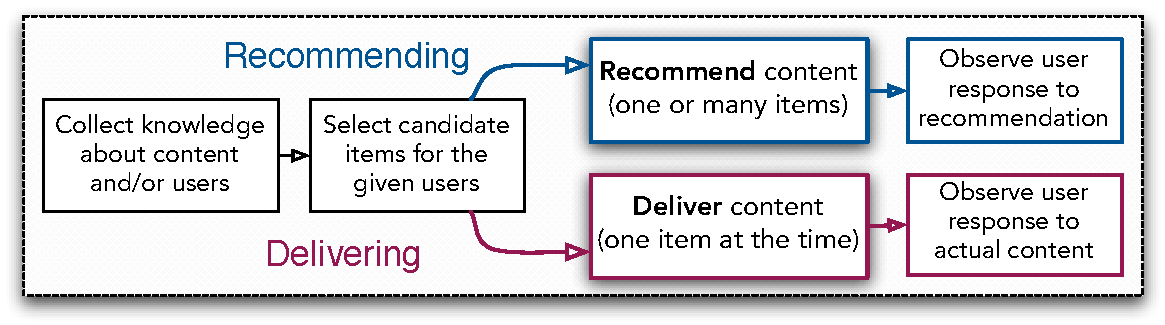
\epsfig{file=img/fig4_2, width=\textwidth}
\caption{Recommender and delivery systems compared.}
\label{fig:recommend_deliver}
\end{figure}

Recommender systems have gained wide attention in relation to the expansion of the World Wide Web, where they have proven helpful for people looking for new movies to watch \cite{Hill95}, songs to listen to \cite{Shardanand94}, news to read \cite{Resnick94}, pages to visit \cite{Lieberman95}, restaurants to check \cite{McCarthy02}, people to know \cite{Terveen05}. %, and in other Web-related applications \cite{Brusilovsky07}.

Delivery is appropriate when items are small, cheap, easily available and storable (e.g., digital audio, digital video, news stories) while items that are large, expensive or not easily available are only recommended (e.g., travel destinations, restaurants, social partners).
Recommender systems can also work on multiple domains at the same time, like InterestMap \cite{Liu05} which simultaneously recommends books, songs, foods, films, television shows and sports based on cross-domain user taste profiles.

Recommender systems often offer unrequested recommendations; for example Amazon constantly presents lists of `recommended books' that customers can completely (and often do) ignore.
By contrast, delivery systems need be prompted by the users for customised content. % to experience. % `on the spot'. For instance, the Web-based music community Last.fm offers personalised radio channels to those users who explicitly ask for a listening experience adapted to their taste.

Since recommender systems do not provide the actual content, an immense collection of items can be recommended without the need for any physical storage. 
For example, MovieLens \cite{Cosley03} recommends movies from a catalogue of 5,600 titles; since movies are recommended\,---\,not delivered\,---\,the system only has to store and transmit the names of the movies, not the real movies.
On the contrary, delivery systems usually require storage and transportation capacity which can limit the range of offer.
%For example, Last.fm personalised radio requires physical space to store the songs, network bandwidth to stream, and a batch process to continuously include newly published songs to the catalogue.

% subsubsection to_recommend_or_to_deliver (end)

\subsubsection{Output: items, sets or sequences} % (fold)
\label{ssub:adaptation_size_and_output}

The outcome of an adaptive system can either be \emph{one} item, a \emph{set} of items, or an ordered \emph{sequence} of items.
%
One item is typical returned when items are expensive (e.g., travels, houses), and the audience can only afford to experience one. 
An example is CATS \cite{McCarthy06b}, which recommends \emph{one} skiing travel destination for a group of friends.

A set of items is commonly returned when items require some time to be experienced (e.g., movies, books). %, and the order in which they are experienced is not paramount. 
For example, MovieLens recommends a \emph{set} of movies to watch and Amazon recommends a \emph{set} of books to read, leaving the users to choose which items to buy and in which order. 
%\cite{Dieterich93} named these systems \emph{user-controlled} adaptive systems.

Finally, a sequence of items is returned when items require a short time to be experienced (e.g., songs, news stories), and the order in which they are experienced is significant. 
For example, Pandora delivers user-adapted Web radio channels with a specific `musical continuity', in the sense that every song is acoustically correlated with the previous song played on the same channel.
% ssubsection adaptation_size_and_output (end)


% [[POTREI TOGLIERE DEL TUTTO QUESTO]]
% \subsubsection{Timing: a priori or continuous} % (fold)
% \label{ssub:timing_continuous_or_discrete}
% 
% User-adaptive systems can either update or not the knowledge content used for the adaptation process. 
% Content-based filtering technique typically estimate all the item-to-item similarity measures beforehand, and do not change them even if users do not appreciate the adaptation proposed. For example, NewsWeeder \cite{Lang95} recommends news stories based on a similarity measure between news item and news item calculated \emph{a priori} using a TF-IDF (Term Frequency - Inverse Document Frequency) approach. Once this measure has been defined, the recommendations are calculated \emph{off-line}, and are not influenced by the user feedback.
% 
% On the contrary, other adaptive systems take into account the response of the audience to improve the customisation on the run. This is mostly true in delivery systems, where immediate user feedback can be obtained to learn whether the adaptation process matched the preference of the public. For example, Pandora.com broadcasts personalised Web radio stations; the selection of the musical sequence is initially focused on maintaining a musical continuity from song to song but, as long as a user starts rating or skipping the proposed songs, the system integrates the user preference in the adaptation algorithm and improves in real time the process producing an even better customised musical stream.

% subsubsection timing_continuous_or_discrete (end)


% subsection user_adaptive_systems (end)


\subsection{Recommender techniques} % (fold)
\label{sub:adaptation_techniques_item_based_and_user_based}

Adaptive systems provide users with content of interest from a potentially overwhelming set of choices.  
Adaptation processes are characterised by different kinds of knowledge representation. % \cite{Brusilovsky96}
A common family of techniques for adaptation is \emph{collaborative filtering}, which consists in presenting a user with content liked by people with a similar profile.
Another family of techniques is called \emph{content-based filtering} and takes place by presenting a user with content similar to items previously liked by the same user.
A third family of techniques, called \emph{knowledge-based}, uses domain knowledge about items' association.

\subsubsection{Collaborative filtering} % (fold)
\label{ssub:collaborative_filtering}

Collaborative filtering techniques select items based on the correlation between people with similar preferences. 
The name ``collaborative filtering'' was proposed by the developers of Tapestry \cite{Goldberg92} and has been used ever since.
The way in which similarity between users is computed depends on the application domain: Amazon interprets similar users as customers who bought the same books in the past, MovieLens as users who rated the some movies likewise.
Once a similarity measure has been defined, the technique works by selecting for each user a set of items liked by people similar to that user.
An interesting comparison of several music-related collaborative filtering systems (Last.fm, Pandora, GhanniMusic, Jango, MeeMix) is presented by \citet{Fox07}.
% COULD REMOVE THIS IMAGE
%\begin{figure}[hbtp]
%\centering \setlength{\abovecaptionskip}{3pt}
%\epsfig{file=img/collaborative_filtering, width=\textwidth}
%\caption{Collaborative filtering.}
%\label{fig:collaborative-filtering}
%\end{figure}


Collaborative filtering is content-agnostic in the sense that the technique is suitable independently of the application domain (e.g., books, music, video).
\citet{Herlocker04} discussed different problems of this approach related to the fact that items cannot be recommended unless users have expressed a preference for them. 
\emph{Cold start} refers to the situation where new items appear and the technique cannot immediately recommend them, since no user rating is available to work on. 
Similarly, when new users join in, the technique needs to learn their preferences before any recommendation can be given. 
\emph{Scarcity} refers to situations where the number of available items is so much larger than the number of users that the coverage of ratings is very sparse and only a few objects are recommendable. 
Another typical problem is for users with \emph{boundary taste} to be provided with poor recommendations since their profiles do not match many other user profiles. 
\emph{Lack of diversity} refers to situations where a collaborative filtering technique suggests a set of items that are intrinsically similar (e.g., five books by the same author, five travels with the same destination) reducing the range of recommendations to a very specific target. 

% subsubsection collaborative_filtering (end)

\subsubsection{Content-based filtering} % (fold)
\label{ssub:content_based_filtering}

Content-based filtering techniques analyse the intrinsic content of every available item and recommend items which are similar to items the user likes. 
The way in which similarity between items is computed depends on the nature of items.
InformationFinder assessed similarity between Web documents comparing the presence of significant phrases \cite{Krulwich96}, while NewsWeeder measured similarity between news stories comparing the frequency of the occurring words \cite{Lang95}.

%Once a similarity measure has been defined, the technique works by selecting for each user a set of items similar to content the user likes.
%% COULD REMOVE THIS IMAGE
%\begin{figure}[hbtp]
%\centering \setlength{\abovecaptionskip}{3pt}
%\epsfig{file=img/content_filtering, width=\textwidth}
%\caption{Content-based filtering.}
%\label{fig:content-based-filtering}
%\end{figure}

Examples of music content-based recommender systems are Mufin, %\footnote{\url{http://mufin.com}}, 
which calculates the similarity between songs comparing properties like tempo, instruments, sound density or harmony \cite{Mufin08}, The Echo Nest, %\footnote{\url{http://the.echonest.com/}}, 
which combines text analysis, audio analysis and user activity \cite{EchoNest09}, and Tangerine, %\footnote{\url{http://www.potionfactory.com/tangerine/}}, 
which works by analysing the BPM and the beat intensity of songs \cite{Tangerine09}.

Content-based filtering is tightly related to the nature of the items to adapt and can obtain good results only in domains where content analysis, parsing and classification have advanced (e.g., text, music), while for complex domains where automatic analysis and categorisation is not yet feasible (e.g., video, interaction data), this is not a suitable approach, since similarities from item to item cannot be drawn as easily.

% subsubsection content_based_filtering (end)

\subsubsection{Knowledge-based techniques} % (fold)
\label{ssub:hybrid_filtering}

Knowledge-based techniques reason about domain knowledge to find items that best match the user needs.
These techniques do not rely on a base of user ratings and are independent of individual tastes.
Instead they have knowledge about how a particular item meets a particular user need, and can therefore reason about the relationship between a need and a possible recommendation \cite{Burke00}.

% From Chun "'THE IMPLEMENTATION OF KNOWLEDGE-BASED RECOMMENDER SYSTEM FOR ELECTRONIC COMMERCE USING JAVA EXPERT SYSTEM LIBRARY"

As \citet{Chun01} pointed out, knowledge-based techniques are appropriate for products like cars, houses, computers, that a person would buy because of knowledge about how an item matches personal requirements rather than because other persons bought that same item.

A music-related knowledge-based system is the Music Genome Projects \cite{Pandora06}.
As a group of trained music analysts listen every day to hundreds of songs and describe their musical qualities ``using up to 400 distinct musical characteristics'', a large knowledge base is built up of relationships between popular themes that serves as the basis for the recommendations provided through Pandora Web radio. % [CITE?].

A sub-category of knowledge-based techniques is composed by % Knowledge-Intensive 
systems that apply Case-Based Reasoning to the task of recommendation.
In these systems, solutions to past problems constitute the knowledge required to provide recommendations for new users.
\citet{Smyth07} summarised advantages of case-based recommender systems, which can converse with the users to better focus on their requirements, evaluate critiques, enhance the diversity of the outcome and explain the reason behind the provided recommendations.
Examples of Case-Based Reasoning recommender systems are Entree \cite{Burke97}, the Wasabi Personal Shopper \cite{Burke99}, Expertclerk \cite{Shimazu01}, WEBSELL \cite{Cunningham01}, Smart Radio \cite{Hayes01b} and the CATS group recommender \cite{McCarthy06b}.


% from burke00


\subsection{Group-adaptive systems} % (fold)
\label{sub:group_adaptive_systems}

Adaptive systems can either be targeted to individuals or to groups.
Extending adaptation processes to groups is a challenging problem, since each member has particular characteristics that should be accounted for. 
\citet{Messick83} pointed out how a group-adaptive system faces the ``social dilemma''  of looking for a compromise between individual and collective interests. 
The system has to find the behaviour that is adequate for the group while taking into account individual preferences of each member.

Group-adaptive systems have appeared in domains other than music, for instance \citet{McCarthy02} described a system that advices a group of friends with a restaurant to attend, \citet{OConnor01} a movie to watch, \citet{McCarthy06b} a tourist attraction to visit. % In all these situations, recommender systems need decide among different options, whereas the members of the group can have heterogeneous preferences towards these options.

The way in which adaptation for the group takes place depends on the characteristic of the group.
\citet{Hill95} distinguished between \emph{co-located} and \emph{displaced} groups.
In the last case, the term ``virtual community'' is more appropriate: people can influence each other as though they interacted but they do not interact, and the system has to maintain displaced members aware of the actions and decisions taken by the group.

\citet{Haseman02} distinguished between \emph{changing} and \emph{stable} groups, meaning that members are allowed or not to join and leave the group. If the composition of a group changes with time, a group-adaptive system might need to inform new members about how previous decisions were made.

\citet{Saklofske89} and \citet{Raghunathan08} remarked how people in a group feel a sense of affiliation with the others and this can positively influence enjoyment from sharing a hedonic activity.
While \emph{intentional} groups take place when people explicitly long for a social experience to share with other people, % for instance when they decide to watch TV with their family, or go dancing with their friends. 
\emph{accidental} groups are made of people who gather with no explicit reason.
\citet{McCarthy98} presented an example of how hard it is to satisfy an accidental group.

%People who do not like Rap music might as well listen to some Rap radio if this makes a friend happy, but they would not do the same for the sake of some complete stranger. 

People in accidental groups are \emph{competitive}, trying to push their individual goals in front of everyone else's, as in political elections. 
In intentional groups, people are instead more \emph{collaborative}, trying to reach a certain degree of group satisfaction.
Intentional groups are generally small groups for which sociologists have found that members may give up part of their individual goals to reach for some group effects, such as conformity, cohesiveness and ``consensuality'' \cite{Hogg96}.

\citet{Chae98} used the term ``narrowcasting'' to describe the situation where media content is delivered to a small group.
In a narrowcasting scenario, people are able to select from a long list of customised channels rather than passively experience a generic broadcast content.
Narrowcasting enables the audience to precisely match the experience with their own views, although \citet{Chaffee01} pointed out how this confines people to live in a ``cocoon of self-reinforcing media''. 

% subsection group_adaptive_systems (end)


\subsection{Preference aggregation} % (fold)
\label{sub:preference_aggregation}

The main challenge for a group-adaptive system is how to combine preferences of multiple persons when they differ.
There are distinct models to aggregate multiple individual preferences in order to assess the ``suitability'' \cite{Jameson07b} of a particular item for a group as a whole. 

Preference aggregation is a multi-person decision making problem that has been broadly covered by social choice theorists \cite{Arrow70}, social psychologists, economists and information scientists \cite{Tindale03,List02}.

% Enric says: we view this as a social choice problem (?)

 %, and has been shown that no judgement aggregation function exists generating ``complete, consistent and deductively closed collective sets of judgements which satisfies universal domain, anonymity and systematicity'' \cite{List02}.

% \begin{figure}[hbtp]
% \centering \setlength{\abovecaptionskip}{3pt}
% \epsfig{file=img/pref_aggr_1, width=\textwidth}
% \caption{Aggregating preferences to select one candidate.}
% \label{fig:preference-aggregation}
% \end{figure}

% Social choice theory aims at finding rules for amalgamating different preferences to ensure certain `desirable properties' \cite{Grabisch98} of the resulting group choice. 

Different approaches proposed to aggregate group preferences include:
introducing social functions that employ some pre-defined aggregation strategy \cite{Masthoff04};
asking users to provide information to determine how the combination can be accomplished \cite{Jameson04};
asking domain experts to guide the combination process \cite{Ardissono03};
promoting social interaction with an interface that allows people to watch, critique, suggest, and discuss recommended items \cite{McCarthy06b}; 
deputing to agent negotiation, with automated agents acting on behalf of humans to generate and form group recommendations \cite{Bekkerman06};
modelling information markets through which group members bet on their judgement about future events \cite{Sunstein05};
developing genetic algorithms \cite{Holland75} to identify the item that best combines individual and group ratings \cite{Chen08}.


%% subsection preference_aggregation (end)

%\subsection{Criteria of fairness} % (fold)
%\label{sub:fairness_of_aggregation_models}

The election of an aggregation function to merge individual preferences is conditioned by the required level of fairness.  
Depending on the application, various rationality principles may apply to select alternatives.

When aggregating multiple individual preferences into a unique group choice, a number of goals are desirable but not always compatible among them, such as matching the preference of the majority, preventing people from leaving the group, maximising average satisfaction, ensuring some degree of fairness, treating group members differently when appropriate, discouraging manipulation of the recommendation mechanism, ensuring comprehensibility and ``acceptability'' \cite{Jameson07b} and minimising misery.
Misery refers to the situation where at least one member of the group is strongly unsatisfied by the aggregation made.

\citet{Chevaleyre07} illustrated different approaches to achieve a degree of fairness in the group, such as \emph{egalitarianism} and \emph{utilitarianism}. 
An egalitarian allocation is driven by the individual utility of the \emph{poorest} agent in the system; aiming at maximising this value is an example for a basic fairness requirement.
An utilitarian allocation is driven by the \emph{sum} of the individual utilities; asking for maximal utilitarian social welfare is a very strong efficiency requirement. 

The weakest possible requirement for preference aggregation is \emph{Pareto efficiency} \cite{Grabisch98}: if at least one individual prefers an item $X$ to an item $Y$ and no one likes $Y$ better than $X$, then the aggregated preference of the group should be higher for $X$ than for $Y$.

Criteria of fairness change when the group-adaptive system does not select \emph{one} item, but rather delivers a whole \emph{sequence} of items, customised for the group.
Behavioural decision theory \cite{Novemsky05} suggests that the mere fact that an outcome is embedded in a sequence might create a frame of reference that can influence subsequent preferences.
In these cases, the history of past aggregations should be taken into account to promote fairness. 
% This is done by Flycasting.

% \begin{figure}[hbtp]
% \centering \setlength{\abovecaptionskip}{3pt}
% \epsfig{file=img/pref_aggr_2, width=\textwidth}
% \caption{Aggregating preferences to select a sequence of candidates.}
% \label{fig:preference-aggregation-sequence}
% \end{figure}

% subsection fairness_of_aggregation_models (end)


%\section{Customising a radio channel for its audience} % (fold)
%\label{sec:what_i_want_to_do}

%\subsection{Problem definition} % (fold)
%\label{sub:problem_definition}

% subsection problem_definition (end)

%The goal of poolcasting is to broadcast on each channel a sequence of songs that is satisfactory for the group of listeners.
%Poolcasting generates this sequence by adding in real time one song after the other. 

%This selection process is driven by four requirements that every played song should match:


% \subsection{Fairness} % (fold)
% \label{sub:aggregating_multiple_preferences2}
% 
% [This subsection should be revised]
% 


\section{The Case-Based Reasoning selection process} % (fold)
\label{sec:the_case_based_reasoning_selection_process}

Poolcasting is a technique to adapt musical content for a group, and is focused around the idea of \textbf{channel}.
A channel represents the virtual space where a group of people gather to listen to music together: a radio channel, a party location, a discotheque.

The persons listening to a particular channel are called the \textbf{audience} of the channel and are indicated with $\mathcal{U}$. 
People are free to join and abandon a channel at different moments: the audience of a channel changes with time. 

The notation $\mathcal{U}_T \subseteq \mathcal{U}$ refers to the set of persons in the channel at a given time $T \in \mathbb{N}^+$ where time is measured counting the songs played so far on the channel: $\mathcal{U}_1$ denotes the audience of the channel while the first song is playing, $\mathcal{U}_2$ while the second song is playing, and so on.

The set of songs available to be played form the \textbf{content} of the channel and are indicated with $\mathcal{C}$.
Similarly to the audience, content can change with time; for instance newcomers can bring more CDs to a party or a radio can buy new records.
The songs available at a particular time  $T \in \mathbb{N}^+$ are indicated with $\mathcal{C}_T \subseteq \mathcal{C}$.

The problem addressed by poolcasting is to play a sequence of songs that matches the four goals of variety, smoothness, customisation and fairness introduced in Sect.~\ref{sec:adapting_music_for_a_group_of_listeners}.
Since both the audience and the content change over time, the musical sequence cannot be entirely scheduled at time $T = 0$ but has to built in real time considering at each moment the available songs and current participants.

%The notation $H_T$ is used to indicate which song is played at time $T$.
Poolcasting follows an \textbf{iterated} decision approach: 
while the first song is playing on the channel, poolcasting decides which will be the second song to play; as soon as the first song ends, the second song starts playing on the channel and poolcasting decides which song will play next, and so on.
%
The way in which poolcasting determines which song to play at any given moment $T$ is by means of a CBR process that is represented in 
Fig.~\ref{fig:iterative_cbr} and whose components (case bases, retrieve, reuse, revise process) are explained hereafter.
%
\begin{figure}[bthp]
\centering \setlength{\abovecaptionskip}{3pt}
%\epsfig{file=img/iterative_cbr, width=\textwidth}
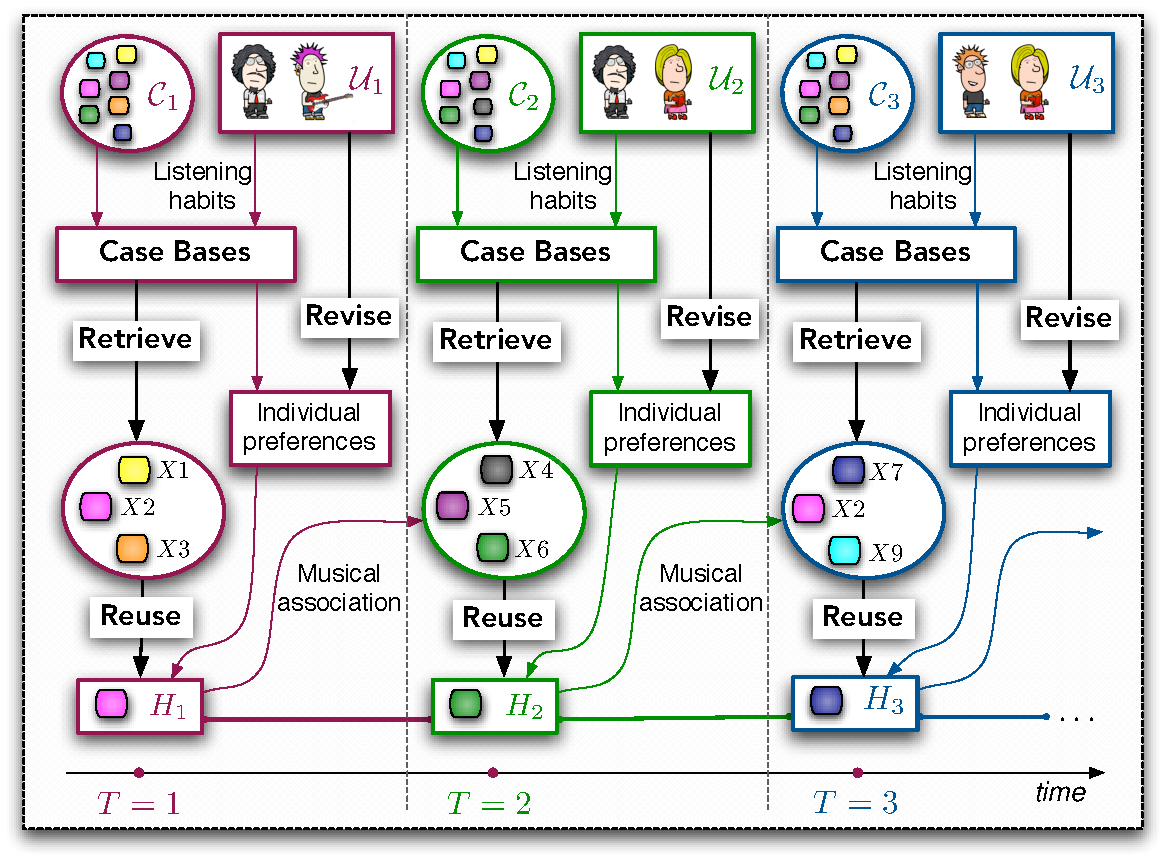
\epsfig{file=img/fig4_3, width=\textwidth}
\caption{The iterative CBR selection process.}
\label{fig:iterative_cbr}
\end{figure}





% To combine all the requirements in real time and solve the iterative social choice problem, poolcasting employs a Case-Based Reasoning (CBR) process.


% \begin{figure}[hbtp]
% \centering \setlength{\abovecaptionskip}{3pt}
% \epsfig{file=img/chap5, width=\textwidth}
% \caption{Chap 5.}
% \label{fig:chap5}
% \end{figure}



\subsection{The case bases} % (fold)
\label{sub:the_case_base_setup2}

In classical CBR, cases consist of (problem $\rightarrow$ solution) pairs;
each new problem is solved independently by retrieving similar past cases and reusing their solutions.

In poolcasting, the `problem' consists in determining which song to play at each time $T$ and cannot be solved \emph{independently} from previous and successive problems. 
In fact the objective is not to find a \emph{single} song that satisfies the audience, but to build a good \emph{sequence} of songs that fulfils variety, smoothness, customisation and fairness.

For this reason, poolcasting does not store in the case base a series of `past problems', but instead valuable knowledge to solve the sequential problem of deciding which song to play at any moment $T$.

Cases in poolcasting are defined as tuples <$X$, $a(X)$, $p(U,X,T)$>, where $X \in \mathcal{C}_T$ is any available song, $a(X)$ its performing artist, and $p(U,X,T)$ is the \textbf{individual preference} of any listener $U \in \mathcal{U}_T$ for the song $X$, that is, how much $U$ would like song $X$ to be played on the channel at time $T$.

Poolcasting is able to estimate the individual preferences of the different participants following the method presented in Chap.~\ref{cha:preferences}.
Every participant supposedly has a personal music library stored in some digital device (e.g., iPod, iTunes) and personal music libraries contain listening habits data indicating which songs a person has most played and voted.
Poolcasting extracts the listening habits data of the audience either from their music players (e.g., from Apple iTunes, see Fig.~\ref{fig:itunes_claudio}) or from the Web  (e.g., from Last.fm profiles, see Fig.~\ref{fig:lastfmprofile}) and infers the implicit preference $i(U,X)$ of each participant for each song, according to the function $i: \mathcal{U} \times \mathcal{C} \to [0,1]$ defined in \eqref{eq:implicit_preference}.
These values are then stored in the case base as individual preferences.

If a participant $V$, for instance, has `Karma Police' (Radiohead) as the top played/top rated track in the Last.fm profile page, then poolcasting stores in the case base the tuple <`Karma Police', Radiohead, 1> as a knowledge of the fact that $V$ would like that song to be played.
If a different participant $Z$ has instead a slightly negative preference for `Karma Police' (Radiohead), then poolcasting creates a second tuple <`Karma Police', Radiohead, $-0.5$> in the case base as a knowledge of the fact that $Z$ would not like that song to be played.

If two different participants have different preferences for the same song (as in the previous example), poolcasting stores both facts since they can both help decide which music to play.
To distinguish between cases related to different participants, poolcasting stores the cases of each participant in a separate case base.
In other words, poolcasting holds a \textbf{collection of case bases}, one for each participant.

%In fact, each personal music library can be seen a case base of previous experiences, namely played and rated songs. A participant sharing personal listening habits data is making available a collection of past experiences, each stored in a different case.

Each participant is treated independently and contributes with a piece of knowledge to the system.
Since participants can join and leave the channel at different moments, the collection of case bases is dynamic:
when new participants join the channel and share listening behaviour data, new case bases become available; when listeners abandon the channel, their case bases leave the collection.
The collection of case bases is determined at each moment by the songs of the current participants in the channel.

% ?? The way in which a participant shares listening habits data 

% 
% In poolcasting, past experience is related to the songs that are shared by the radio participants. 
% The shared library of each participant $U$ is considered as a Case Base, where one case corresponds to each song $X$ with its implicit preference $i(U,X)$ estimated from the analysis of the personal library as explained in Chap.N.
% 
% Every Case Base contains the list of songs in the shared library of a participant and a preference degree for each song.
% Overall, the radio has a \textbf{collection of case bases} which is dynamic because when listeners join or leave the radio and share or `unshare' their libraries, new case bases enter or leave the collection.
% 
 
% subsection the_case_base_setup2 (end)

\subsection{The retrieve process}

% When, at moment $T$, poolcasting has to decide which song to play next on the channel, it can selects one song among those available in the collection of case bases at time $T$.
% However, not \emph{all} the songs shared by the audience can be played on \emph{any} channel; for instance a channel defined as `genre = Rock' (see Fig.N) only admits `Rock' songs.
% 
% The set of songs that can actually be played on a channel at a given moment $T$ (that is, songs in shared libraries at time $T$ that match the definition of the channel) is indicated with $\mathcal{C}_T$.

The retrieve process is meant to identify at time $T$ which available songs  are \textbf{good candidates} to be played next on the channel.
The retrieve process addresses the goals of variety (\ref{p:variety}) and smoothness (\ref{p:smoothness}) with two subsequent steps: 
first each song is rated with a \emph{relevance value} $k: \mathcal{C} \times \mathbb{N}^+ \to [0,1]$ that expresses how much the song satisfies the requirements of variety and smoothness; then the $\kappa$ best rated songs are retrieved.

Every song $X \in \mathcal{C}_T$ that does not fit the channel constraints is assigned the lowest possible value $k(X,T) = 0$ to prevent that song from being played.
For instance, if a channel is defined as `Rock' then every non-Rock song gets a relevance value of 0; if a channel is defined as `Italian' then non-Italian tracks are assigned a value of $k(X,T) = 0$.

Every song recently played on the channel, or by a recently played artist, is also assigned a relevance value of 0.
This is intended to guarantee the requirement of variety.
Formally, let $H_J$ be the $J$-th song played in the channel, and let $[H_1, H_2, \ldots, H_{T-1}]$ be the list of songs played so far.
Then $k(X,T) = 0 \; \forall X \in [H_{T-\eta}, H_{T-\eta+1}, \ldots, H_{T-1}]$ (recently played songs) and $k(X,T) = 0 \; \forall X\,|\,a(X) \in [a(H_{T-\zeta}), a(H_{T-\zeta+1}), \ldots, a(H_{T-1})]$ (recently played artists).
The parameters $\eta \in \mathbb{N}^+$ and $\zeta \in \mathbb{N}^+$ determine the number of songs that have to pass before the same song or artist can be played again in the same channel.
The values of these parameters are defined according to the channel; $\zeta$ is small when the same artist is allowed to repeat (e.g., a `Frank Sinatra' channel), while a high $\eta$ characterises channels that strongly avoid repeating the same tracks (e.g. a `Dance' channel). 

Next, the retrieve process assigns a relevance value to the remaining songs according to how well they would go in a sequence after the last song played $H_{T-1}$. 
This is intended to guarantee the requirement of smoothness and is accomplished is by exploiting the co-occurrences analysis of playlists explained in Chap.~\ref{cha:smoothness}.
The idea is that the more people have played two songs together in their daily activities, the more two songs appear closely in playlists, the more they `go well' together in sequence and the more it makes sense to reproduce them one after the other in a channel to guarantee smoothness.
Formally, each remaining song $X$ in the collection of case bases is assigned a relevance value of $k(X,T) = s(H_{T-1}, X)$ that indicates how much $X$ would sound well in a sequence after the last song played $H_{T-1}$, where the function $s: \mathcal{C}^2 \to [0,1]$ was defined in \eqref{eq:final_degree}.

Having determined a relevance value $k(X,T)$ for each song $X \in \mathcal{C}_T$, the $\kappa$ songs with the highest value are identified as the best candidate songs to become $H_T$ (the next song to play).
The cases that contain these songs are retrieved and constitute the \emph{retrieved set}.

% subsection the_retrieve_process3 (end)

\subsection{The reuse process} % (fold)
\label{sub:the_reuse_process3}

The reuse process is meant to adapt the retrieved set to the preferences of the current audience. % in order to select the song that best address the requirements of customisation and fairness.
In this process, the songs in the retrieved set are \textbf{ranked} according to how much the current listeners like each song: % (\ref{p:customisation}) with an aggregation strategy defined to satisfy every listener in the long run (\ref{p:fairness}).
the top ranked song is identified as the candidate preferred by the group of listeners `as a whole'.

To know how much \emph{the group} likes each candidate song, poolcasting reuses the individual preferences $p(U,X,T)$ stored in the retrieved cases.
Every case contains knowledge about \emph{one} participant.
Poolcasting aggregates cases by candidate song to measure how much the whole group likes each candidate.


%For each candidate song $X$, poolcasting aggregates the preferences of all the current participants into a \textbf{group preference} function $g: \mathcal{C} \times \mathbb{N}^+ \to [-1,1]$ that measures how much the group `as a whole' would like to listen to a specific song $X$ at time $T$.

Several strategies exist to aggregate preferences in a group. %, which differ in the way they address the problem of fairness.
A common strategy is \emph{plurality voting}, which consists in ranking first the items preferred by the majority. 
With this approach, the preferences of the minorities never affect the determination of the best ranked item; in other words plurality voting does not endeavour to equally satisfy \emph{all} the participants.

%The main problem of plurality voting is that people with boundary preferences are completely ignored, since they do not belong to the majority.

Poolcasting uses a different strategy which combines instead the preferences of all the members of the audience, assigning more importance to those participants that were less satisfied by the last songs played.

This strategy\,---\,called satisfaction-weighted aggregation and explained in Sect.~\ref{sec:social-choice-problem}\,---\,returns for each candidate song $X$ a group preference degree $g(X,T)$ that measures how much the group as a whole would like song $X$ to be played at time $T$ on the channel.

Given this group preference function, the reuse process ranks each song $X$ in the retrieved set according to $g(X,T)$.
The best ranked song is identified as the best candidate to become $H_T$, the song that will play next on the channel.

% The `optimal' situation would be to have at least one retrieved song $Y$ that every current listener loves, that is, such as $p(U,Y,T) = 1 \forall U \in \mathcal{U}_T$. In this case, the song $Y$ would clearly be played next on the channel as this would satisfy the entire audience.
% 
% Still this situation is quite uncommon: even close friends often have different preferences for different songs and hardly one song can be found that everyone agrees upon, especially when the group is large.
% 
% In this case, the group has to accept a \textbf{compromise}: a song will be played that not everyone loves but that, hopefully, will not either be too distant from anyone's taste.
% Finding the right compromise is the most critical challenge for poolcasting: to identify the song in the retrieved set that the current audience `as a whole' most likes.
% 
% This means to combine in some way the preferences of all the listeners in order to find the retrieved song that has the highest `group preference'. 
% 
 
\subsection{The revise process} % (fold)
\label{sub:the_revise_process2}

So far, the CBR process has required no interaction from the participants.
The retrieve process has automatically picked a subset of good candidate songs that have been ranked in the reuse process according to the preferences stored in the case bases. % and the best ranked song is pre-selected to play next.
%If no additional feedback is provided, the best ranked song will be automatically uploaded to the radio server and played as soon as the previous song will have finished.

At this point, poolcasting asks the members of the audience to express feedback about the proposed ranking.
While some participants might agree with the top ranked candidate, others might prefer a different candidate song to be played.
By reviewing their preferences for the candidates, participants can alter the ranking and make a different song play next.

The revise process consists in collecting explicit feedback from the current participants about the available songs. 
\textbf{Explicit feedback} is indicated with the function $e: \mathcal{U} \times \mathcal{C} \times \mathbb{N}^+ \to [-1,1]$, where $e(U,X,T)$ denotes the last preference expressed by a participant $U$ for a song $X$ before time $T$.

The exact value of $e(U,X,T)$ depends on the type of feedback provided: $e(U,X,T) = 1$ denotes a participant $U$ who stated `unconditional love' for a song $X$; $e(U,X,T) = 0$ represents indifference; $e(U,X,T) = -1$ indicates that $U$ does not want at all $X$ to be played. 
Other values between $-1$ and $1$ mean milder negative and positive preferences. 

Explicit feedback serves to update the individual preferences $p(U,X,T)$ stored in the case bases. 
By default these preferences are inferred from personal listening habits, but if a participant explicitly states a feedback about a song, then the implicit preferences are replaced with explicit ones. 
Formally, the value of the individual preference degree $p: \mathcal{U} \times \mathcal{C} \times \mathbb{N}^+ \to [-1,1]$ is determined as follows:
\begin{equation}
\label{eq:preference_model2}
p(U,X,T) = 
\begin{cases}
e(U,X,T) & \text{if $e(U,X,T)$ is defined}\\        
i(U,X) & \text{otherwise.}
\end{cases}
\end{equation}

As listeners state their preferences for the candidate songs, the ranking calculated by the reuse process is bound to change. 
For instance, if many listeners vote positively for a given candidate song, that song might become the new top ranked candidate.
A similar outcome can occur if many participants vote negatively for the original top ranked song.

The revise process lasts for a finished period of time;
when the time is over, the best ranked song is finally confirmed as \emph{the} song $H_T$ that will play next on the channel. 
This concludes the CBR process to select the $T$-th song to play, while the process to select the $T + 1$-th song starts right after.

% subsection the_revise_process2 (end)

\section{The iterated social choice problem} % (fold)
\label{sec:social-choice-problem}


% [the key: the reuse, so decisions are not to be independent, what happens with music is that they are not independent!]

The goal of poolcasting is to generate a musical sequence customised for a given audience. 
Poolcasting determines which songs to play iterating the CBR process:
first, song $H_1$ is selected, then song $H_2$, and so on. 
%As a result, the participants get to listen to the musical sequence $[H_1, H_2, \ldots]$, automatically selected without the need for a DJ.

Each song belongs to a retrieved set of candidates that were not recently played and that go well after the last song played; this addresses the goals of variety (\ref{p:variety}) and smoothness (\ref{p:smoothness}).
Moreover each played song is the top ranked according to the combined preferences of the audience; this addresses the goal of customisation (\ref{p:customisation}).

The way in which multiple preferences are combined determines the degree in which fairness is addressed (\ref{p:fairness}).
The objective is to have every participant satisfied in the long run;
therefore if some participants are not satisfied by the music played at a given moment, poolcasting should \textbf{reward} them by playing songs they like.
In this way, everyone might listen to some of their favourite songs after a certain time.

Since the decision about which song is played is determined by the ranking of the candidate set, and since this ranking depends on the preferences of the audience, a way to reward unsatisfied participants is to aggregate preferences using a weighted average that assigns higher weights to less satisfied participants.


\subsection{Group preference degree} % (fold)
\label{sub:the_group_preference_degree}

The strategy to aggregate multiple individual preferences is called \textbf{satisfaction-weighted average}, and consists in averaging individual preferences with a weight that is inversely related to a participant's satisfaction. 

Formally, let $q(U,T)$ indicate the individual satisfaction of a participant $U$ at time $T$; the aggregated group preference is defined as:
\begin{equation}\label{eq:group_with_misery}
\sum_{U \in \mathcal{U}_T}\left( 1-q(U,T-1) \right) \cdot \cfrac{p(U,X,T)}{\#(\mathcal{U}_T)}\,.        
\end{equation}
This weighted average combines for each song $X$ the individual preferences $p(U,X,T)$ of all the members of the audience $\mathcal{U}_T$, where the weight $(1 - q(U,T-1))$ is inversely related to the satisfaction of each person.
%
The function $q(U,T)$ that measures individual satisfaction is formalised hereafter.

%A formal definition of the individual satisfaction degree $q: \mathcal{U} \times \mathbb{N}^+ \to [0,1]$ is described hereafter.

% subsection the_group_preference_degree (end)

% section the_technique (end)
\subsection{Individual satisfaction degree} % (fold)
\label{sec:calculating_individual_satisfaction}

%The first thing that is required to fairly aggregate different individual preferences is to estimate how much each listener is \emph{satisfied} with the music played so far, so that less satisfied listeners can be favoured more later on.

%The function  $q: \mathcal{U} \times \mathbb{N}^+ \to \{0,1\}$ represents the    \textbf{individual satisfaction} degree of a listener for the music played so far on a channel. The more a listener $U \in \mathcal{U}_T$ liked the songs played before time $T$, the higher the value of $q(U,T)$, and vice versa.

The individual satisfaction $q: \mathcal{U} \times \mathbb{N}^+ \to \{0,1\}$ is defined as a combination of individual preferences for the songs played so far in the channel.
In this combination, recent songs are assigned a higher importance since human satisfaction is an emotion that decays with time: people tend to forget remote experiences and be mostly affected by recent ones \cite{Masthoff06}.
The measure
\begin{equation}\label{eq:satisfaction_wrong}
  \sum_{J = 0}^{T-1} \chi^{J} p(U,H_{T-J},T-J)
\end{equation}
formalises this decay model: the individual preferences $[p(U,H_1,1)$, $p(U,H_2,2)$, $\ldots]$ of a listener $U$ for the songs played on the channel are averaged with a weight $\chi^J$ directly related to their recency, where
$\chi \in [0,1]$ is a parameter that determines the degree in which the recency of an experience influences its impact on satisfaction.
Note that when $\chi = 0$ only the last song played has an impact\footnote{When $\chi=0$, the first term of the sum contains $0^0$, which is defined as $1$ in this context.} while when $\chi = 1$ every song has equal impact.

There are three issues to consider about \eqref{eq:satisfaction_wrong}.
%
%The first issue is that the formula equals zerodoes not specify the \textbf{initial satisfaction} of the participants, that is, how satisfied a person
%
The first is that the formula combines the preferences of a participant towards \emph{all} the songs played on the channel, from $H_1$ to $H_{T-1}$.
Nevertheless, every participant is free to join and leave the channel at different moments, and only the preferences for the songs played \emph{while $U$ was listening} should determine the satisfaction of $U$.
For this reason, a \textbf{channel membership} function $m: \mathcal{U} \times \mathbb{N}^+ \to \{0,1\}$ is introduced to identify current listeners at time $T$:
\begin{equation*}
%\label{eq:channel_membership}
m(U,T) = 
\begin{cases}
1 & \text{if $U$ is a member of the channel audience at time $T$}\\        
0 & \text{otherwise}
\end{cases}
\end{equation*}
%for $T \geqslant 1$, while $m(U,0) = 1$ by convention.
and is integrated into \eqref{eq:satisfaction_wrong} to yield the formula:
\begin{equation}\label{eq:satisfaction_wrong_2}
  \sum_{J = 0}^{T-1} \chi^{J} p(U,H_{T-J},T-J) m(U,T-J)\
\end{equation}
that aggregates only the preferences of $U$ for the songs played on the channel while $U$ was listening.

%The second issue is that \eqref{eq:satisfaction_wrong_2} equals zero for every participant that has not yet listened to any song. Still, it should be accounted that people joining a channel for the first time are possibly not quite satisfied since they have not yet listened any good song. For this reason, an \textbf{initial satisfaction} degree $\iota \in [0,1]$ is  introduced that models how much each listener is satisfied at time $T = 0$. This value is integrated into \eqref{eq:satisfaction_wrong_2} and the formula rewritten as: 
%\begin{equation}\label{eq:satisfaction_wrong_3}
%  \sum_{J = 0}^{T-1} \chi^{J} p(U,H_{T-J},T-J) m(U,T-J) + \chi^{T}\iota\,.
%\end{equation}

The second issue is that \eqref{eq:satisfaction_wrong_2} yields values in the interval $[-(1-\chi)^{-1}, (1-\chi)^{-1}]$, while the desired satisfaction degree $q(U,T)$ yields values in $[0,1]$.
For this purpose, first a normalised version $h: \mathcal{U} \times \mathbb{N}^+ \to [0,1]$ of the individual preference for the played songs is defined:
\begin{equation*}
h(U,T) = \frac{1}{2} \left( p(U,H_T,T) + 1 \right) m(U,T)
\end{equation*}
where the more $U$ liked song $H_T$, the closer to 1 the value of $h(U,T)$, while $h(U,T) = 0$ if $U$ was not listening to the channel while $H_T$ was playing.
%
Next \eqref{eq:satisfaction_wrong_2} is rewritten integrating this notation, as follows:
\begin{equation*}
 \sum_{J = 0}^{T-1} \chi^{J} h(U,T-J)
\end{equation*}
and finally this measure is divided by the sum of its weights in order to yield values in $[0,1]$:
\begin{equation}\label{eq:satisfaction_wrong_4}
 \cfrac{\sum_{J = 0}^{T-1} \chi^{J} h(U,T-J)}
       {\sum_{J = 0}^{T-1} \chi^{J} m(U,T-J)}\,.
\end{equation}

The third issue is that \eqref{eq:satisfaction_wrong_4} is undefined for any participant that has not yet listened to any song, since the denominator equals zero.
To solve this problem, a default \textbf{initial satisfaction} degree $\iota \in [0,1]$ is introduced that models how satisfied a participant possibly is before listening to any song. % at time $T = 0$.
% This value is supposedly small since people joining a channel have not yet listened to any favourite song.
This value is integrated into  \eqref{eq:satisfaction_wrong_4} and the formula rewritten as:
\begin{equation*}
 \cfrac{\sum_{J = 0}^{T-1} \chi^{J} h(U,T-J) + \chi^T \iota}
       {\sum_{J = 0}^{T-1} \chi^{J} m(U,T-J) + \chi^T}\,.
\end{equation*}

This notation can be further reduced introducing the conventions that $m(U,0) = 0$ and $h(U,0) = \iota$.
Replacing in the numerator $\chi^T \iota$ with $\chi^T h(U,0)$ and, in the denominator, $\chi^T$ with $\chi^T m(U,0)$ eventually leads to define the individual satisfaction degree $q: \mathcal{U} \times \mathbb{N}^+ \to \{0,1\}$ as:
\begin{equation}
\label{eq:individual_satisfaction}
q(U,T) = \cfrac{\sum_{J = 0}^{T} \chi^{J} h(U,T-J)} {\sum_{J = 0}^{T} \chi^{J} m(U,T-J)}\,.
\end{equation}

Individual satisfaction increases whenever a song that a participant likes is played, while decreases after listening to a disliked song.
The impact of the last song played over satisfaction is not totally clear in  \eqref{eq:individual_satisfaction} but can be unfolded rewriting the function in a recursive form that defines $q(U,T)$ only from the previous satisfaction degree % at time $T>1$ 
$q(U,T-1)$ and from the preference $h(U,T)$ for the last song played:
\begin{equation}
%\label{eq:recursive_satisfaction}
   q(U,T) = q(U,T-1) + \cfrac{h(U,T) - q(U,T-1) m(U,T)} {\sum_{J=0}^{T} \chi^J m(U,T-J)} \,.
\end{equation}
This notation shows how every new song contributes with a `delta' to the satisfaction of a participant.
The impact of this delta (the second addend of the formula) is mostly determined by the decay parameter $\chi \in [0,1]$.
%
If $\chi$ is small, the impact is strong, which means that satisfaction can change rapidly over time. 
At the extreme, if $\chi = 0$, then $q(U,T) = h(U,T)$, which means the satisfaction of a participant is solely determined by the last song played.
%
On the other hand, if $\chi$ is large, then the impact is weak and satisfaction can only change slowly over time.

Figure~\ref{fig:satisfaction_decay} illustrates this behaviour with an example: 
the %red
solid line plots the preferences $h(U,T)$ of a person $U$ for 25 songs played on the channel, 
the %blue 
dotted line plots the satisfaction degree of $U$ modelled using a small decay value ($\chi = 0.2$);
the %green 
dashed line plots the same satisfaction function modelled using a large decay value ($\chi = 0.8$). 
The dotted line is sharper and responds almost immediately to the changes of $h(U,T)$, corresponding to a model of `immediate satisfaction'.
The dashed line is instead softer and more influenced by the whole history of $h(U,T)$, corresponding to a model of `long-term satisfaction'.
%
\begin{figure}[bthp]
\centering \setlength{\abovecaptionskip}{3pt}
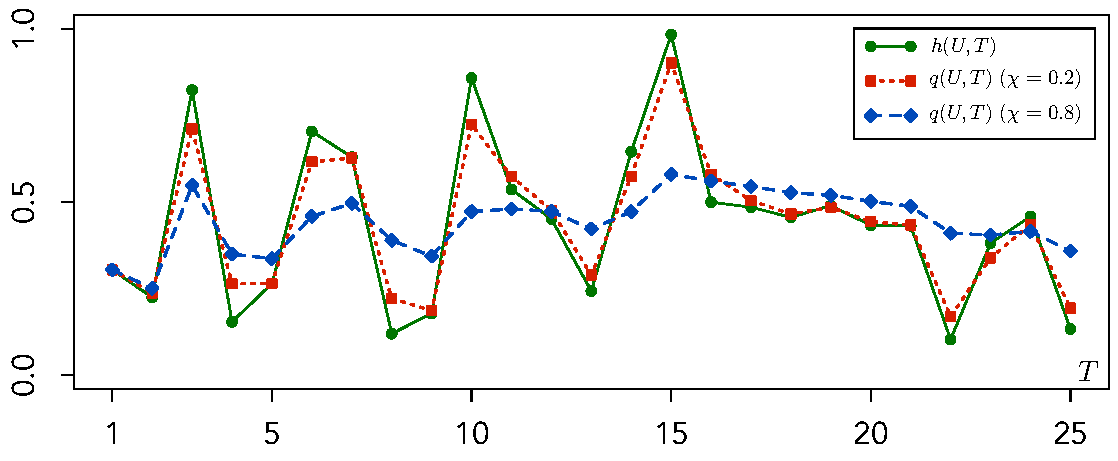
\epsfig{file=img/fig4_4, width=\textwidth}
\caption{Influence of the decay parameter $\chi$ on individual satisfaction.}
\label{fig:satisfaction_decay}
\end{figure}

% section calculating_individual_satisfaction (end)

\subsection{Satisfaction-weighted aggregation without misery} % (fold)
\label{sub:how_we_fairly_aggregate_preferences}

As defined in \eqref{eq:group_with_misery}, the individual satisfaction degree \eqref{eq:individual_satisfaction} serves to weigh the influence of different participants when deciding which song to play next on the channel.
%
This satisfaction-weighted strategy is intended to provide everyone (even participants with boundary musical tastes) with the chance to listen to some favourite songs.

One drawback of this strategy is that even songs that some participants `detest' are bound to be selected. 
In other words, the fact that a participant has the lowest possible preference $p(U,X,T) = -1$ for a given song $X$ does not prevent that song from being played if other participants with higher weights like it.
%
As a result, \emph{misery} can occur, which means that some persons are faced with items they do not wish to experience (songs they would not like to hear).

This situation can be avoided introducing a \textbf{misery threshold} $\mu \in [-1,0]$ that specifies the minimum individual preference that any member is willing to accept for a song.
If any member of the audience has a preference for a song below this threshold, then that song is not played, independently of how much the remaining audience likes that song.

Integrating this threshold into \eqref{eq:group_with_misery} brings to complete the definition of the \textbf{group preference} degree $g: \mathcal{C} \times \mathbb{N}^+ \to [-1,1]$ as:
\begin{equation*}%\label{eq:group_preference}
  g(X,T) =      
\begin{cases}
-1 & \text{if $\exists U \in \mathcal{U}_T :$}\\
& \text{$p(U,X,T) < \mu$}\\        
\rule[-1em]{0pt}{4em} 
%\displaystyle\sum_{U \in \mathcal{U}_T} \frac{q(U,T-1) + 1}{2} p(U,X,T) & 
\sum_{U \in \mathcal{U}_T}\left( 1-q(U,T-1) \right) \cdot \cfrac{p(U,X,T)}{\#(\mathcal{U}_T)} & \text{otherwise.}
\end{cases}
\end{equation*}

To conclude, the strategy of poolcasting to address customisation (\ref{p:customisation}) is to rank the retrieved set according to the group preference and to play the top ranked song.
In order to achieve fairness (\ref{p:fairness}), group preference is calculated with a weighted average that favours members that were less satisfied by the recent channel experience.
Moreover, songs with very low individual preferences are avoided to prevent misery. 

This preference aggregation strategy is iteratively used in the CBR selection process to generate a musical sequence made of songs that, over time, can satisfy the entire audience.

% subsection how_we_fairly_aggregate_preferences (end)

% section the_technique (end)



\section{Summary} % (fold)
\label{sec:contributions_c}

This chapter has described poolcasting, an automatic technique to adapt a sequence of songs to a specific audience.
Most automated music selection techniques are not influenced by the actual listeners, while poolcasting delivers a sequences of songs customised for the audience.
This is achieved by means of a CBR process, where the retrieve and reuse processes have been reinterpreted to generate a \emph{sequence} of solutions adequate for a \emph{group} of users.

The retrieve process does not look for \emph{similar} cases but searches for \emph{good candidates} for the sequence, employing the musical associations calculated in Chap.~\ref{cha:smoothness}.
The reuse process does not adapt \emph{one} retrieved case but customises the retrieved set for the audience aggregating their music profiles assessed as described in Chap.~\ref{cha:preferences}.
%In this way, I deal with the social choice problem of combining multiple individual preferences to make everyone satisfied in the long run.

%Poolcasting works in a dynamic context where members of the audience can join or leave the channel at different moments and new songs can become available over time. The preferences of the listeners are automatically inferred from listening habits and can be explicitly revised at any moment by the audience.

Multiple individual preferences are combined with a satisfaction-weighted aggregation strategy that assigns different weights to different participants based on their satisfaction degree.
The novelty of this aggregation strategy is that \emph{memory} of past elections is accounted for in order to achieve fairness in the long run.
The selection of each song depends on the previous songs selected and on their impact on listeners.
%
The outcome is that individuals might occasionally be confronted with songs they do not like to keep the rest of a group happy, but are soon rewarded with some of their favourite songs.
%The proposed strategy is particularly fit for groups willing to \emph{collaborate} and give up a bit of their individual preferences in order the make the experience satisfactory for everyone: no one will like \emph{all} the songs played, but everyone will enjoy the fact that everyone is having a good time.

The next chapter presents a real-world scenario where the poolcasting technique has been applied.

%Poolcasting avoids playing songs that any participant strongly dislikes in order to avoid misery.




% section contributions_c (end)

% subsection explicit_preferences2 (end)


%The satisfaction of each listeners for the channel at a given moment can be formalised as an \textbf{individual satisfaction} degree $q: \mathcal{U} \times \mathbb{N}^+ \to [-1,1]$, where $q(U,T)$ indicates \emph{how much} a listener $U$ is satisfied with the channel after $T$ songs have been played. Chap.N explains how poolcasting is able to estimate this degree from the analysis of the history of the individual preferences of each listener, and how satisfaction degree is used to favour at each moment less satisfied listeners in the selection of the next song to play.
% 
% 
% Processes of the CBR poolcasting technique
% 
% 
% 
% 
% \subsubsection{The Retrieve Process} % (fold)
% \label{ssub:variety}
% 
% In the retrieve process, poolcasting first excludes from $\mathcal{C}_T$ every song that has been played recently or whose artist has been played recently on the channel, then selects a set of songs which sound well after the last song played $H_{T-1}$.
% 
% In order to do this, poolcasting needs a domain knowledge about which songs sound well together after the last song played on a channel. 
% For instance, poolcasting needs to know that if `True Colors' by Cyndi Lauper is playing on a channel, then `Holiday' by Madonna is a good musical choice to play next, while `One' by Metallica is not.
% A DJ knows from experience.
% In the case of poolcasting, I will explain in Chap.N how this knowledge is automatically extracted from the analysis of playlists collected from the Web.
% Playlists are a way to organise music and poolcasting assumes that the more two songs occur closely and together in playlists, the more they sound well together. % according to a sort of `wisdom of the crowd'.
% In Chap.N we will see how analysing a large set of playlists, poolcasting is able to estimate for each pair of songs a \textbf{musical association} degree $s: \mathcal{C} \to [0,1]$ where $s(X,Y)$ measures \emph{how much} a song $Y$ sounds well after a song $X$ in a sequence.
% 
% Given this function, the songs $X \in \mathcal{C}_T$ with the highest musical association degree $s(H_{T-1}, X)$ are those that best help achieve the goal of smoothness and that are selected in the retrieve process.
% 
% % subsubsection musical_association (end)
% 
% \subsubsection{The Reuse process} % (fold)
% \label{ssub:customisation}
% 
% 
% % subsubsection fairness (end)
% 


% section what_i_want_to_do (end)


% section what_i_have_done (end)


%\section{The Case-Based Reasoning approach} % (fold)
%\label{sec:the_cbr_song_scheduler}

% The strategy of poolcasting to decide which song to play on a radio channel at a given moment is to select a song that fulfils the four requirements listed in Sect.~\ref{sec:what_i_want_to_do}: variety, smoothness, customisation and fairness.
% 
% % To fulfil variety (\ref{p:variety}), poolcasting excludes songs and artists that were recently played. For instance, if `Holiday' by Madonna is playing on a channel, poolcasting avoids playing next `Holiday' or any other song by Madonna.
% 
% 
% 
% 
%% subsection the_case_based_reasoning_approach2 (end)


% chapter poolcasting_web_radio (end)

\chapter{Group-customised Web radio} % (fold)
\label{cha:poolcasting_web_radio2}
\songquote{It's that same sing song on the radio\\
It makes me sad}{R.E.M., 1991} 
\section{Adapting online radio channels to their audience} % (fold)
\label{sec:what_i_have_done}

The previous chapter presented poolcasting, an intelligent music selection technique that automatically decides which music to play in contexts where people listen to music in group (discos, parties, radios, bars, offices).
 
This chapter focuses on the domain of online radios, presenting a novel Web radio framework that employs the poolcasting technique to customise radio music channels for their audience.

Most online radios cannot afford expert DJs to programme their channels and are scheduled with random sequences of songs of a given type (e.g., `Rock' songs in a `Rock' music channel).
Employing an intelligent technique like poolcasting can significantly improve the quality of the music in terms of variety, smoothness, customisation and fairness.

Poolcasting Web radio autonomously schedules music channels with good successions of songs and enables listeners to interact among them and with the system in ways that are inconceivable in other Web radios.
To name a few, listeners can:
\begin{itemize}
 \item contribute with new songs to the music broadcast by the radio;
 \item define new radio channels that match their musical tastes; and
 \item evaluate the available songs to influence the music played.
\end{itemize}
%
The breakthrough of Poolcasting Web radio is the creation of a \textbf{social radio} experience.
Listening to radio is normally an individual activity: people ignore who else is listening, cannot interact with each other or control music but for the volume knob.
Most radio stations, both terrestrial and online, are not affected by \emph{who} is actually connected and listeners are forced to waste time in quest of an `ideal' channel.

Poolcasting Web radio takes instead inspiration from digital music services which broadcast music streams that are \emph{personalised} for the audience. 
These services (e.g., Last.fm, Pandora) offer \emph{private} music channels targeted to individuals, while Poolcasting Web radio provides \emph{public} radio channels customised for multiple simultaneous listeners, enabling friends to enjoy music together. % without the need for a DJ. 
Poolcasting Web radio merges the distributed nature of online radios with the personalised nature of music recommenders. 
%Its particular features are detailed hereafter.
%, providing radio channels that everyone can listen to, where the musical content of each channel is customised in real time for the group of listeners.


% 
% \section{Social interaction: active participants}\label{subsection:active}

% subsection passive_listening4 (end)

% section interactive_features_ (end)

\section{Previous work} % (fold)
\label{sec:previous_work9}

Poolcasting Web radio is a user-adaptive system that delivers customised music to a group.
Previous music-related group-adaptive systems are reviewed hereafter, and a characterisation of Internet radios is provided.

\subsection{Group-adaptive systems in music} % (fold)
\label{sub:similar_applications}

A list of previous systems and prototypes designed to adapt music experience to a group of listeners is reviewed hereafter.

\paragraph{MusicFX} % (fold)
\label{par:musicfx_mccarthy98}
\cite{McCarthy98} was a system that automatically selected which radio station to play in a gym according to the taste of the current attendants.
The domain knowledge was made of a set of 91 radio stations categorised by musical style (`Album Rock', `Beach Party', `Flamenco', etc.); user profiles were built by hand, with each member specifying preference for each musical genre; the aggregation was computed using a weighted random selection policy, prohibiting the system from playing any station for which anyone present had a low rating and limiting the period of time that any one genre could play, in order to increase diversity. 
%The main problems of MusicFX are: requires explicit preferences, needs to satisfy one large (possibly heterogeneous) group, individual preferences are not normalised by average user behaviour, and the system has no memory of past user satisfaction, as the authors report:  ``The group preference arbitration algorithm makes its decision based on current information only. I believe that incorporating historical information could improve its decisions''. For instance, the MusicFX system tries to select the right radio station for people working out in a gym at a given time. 
The main lesson learnt from MusicFX was that people had limited desire in compromising their musical preferences with those of some stranger with whom they just happened to work out with.
% paragraph musicfx_mccarthy98 (end)

%\paragraph{hpDJ} % (fold)
%\label{par:hpdj}
%..
% % paragraph hpdj (end)


\paragraph{Smart Radio} % (fold)
\label{par:smart_radio}
\cite{Hayes01b} was a Web-based client-server application to share compilations of music.
%The idea behind Smart Radio is too encourage the sharing of music programmes using automated recommendation techniques
Smart Radio combined automated collaborative filtering and Case-Based Reasoning techniques.
% The differences are: the unit of recommendation is a playlist of 10 music tracks, not a continuous stream of music; only knowledge from the listening history of the participants is considered, no domain knowledge coming from social Web; for the user profile, they only do this: ``By using the most recently played playlist as an indicator of the user's current interests I also solve the practical problem of having to develop a user-profile representation which is compatible with the representation used by the playlists.''; they consider feature such as genres, not genre affinity degrees.
User ratings were gathered combining explicit and implicit feedback. 
Participants could explicitly choose to rate individual tracks or programmes, while the system implicitly gave a positive rating to songs that had been saved to a user's profile and to programmes built from scratch by a user. %Programmes can be put together in a matter of seconds by simple clicking on the desired music item and adding it to the current play list.'' \cite{Hayes01b}.
% paragraph smart_radio (end)


\paragraph{Flytrap} % (fold)
\cite{Crossen02} was an active environment that gathered users' musical tastes and automatically constructed a soundtrack to please everyone in the same room. 
The system combined domain knowledge about how genres of music interrelate and social knowledge about what kinds of transitions between songs people tend to make and broadcast music that satisfied user preferences while fitting its own notion of smoothness.

%Applications: ``Flytrap is an active environment that knows its users' musical tastes and can automatically construct a soundtrack that tries to please everyone in the room. The system works by paying attention to the music that people listen to on their computers. Users of the system have radio frequency ID badges that let the system know when they are nearby. Using the preference information it has gathered from watching its users, and knowledge of how genres of music interrelate, how artists have influenced each other, and what kinds of transitions between songs people tend to make, the ``virtual DJ'' finds a compromise and chooses a song. The system tries to satisfy the tastes of people in the room, but it also makes a play list that fits its own notion of what should come next. Once it has chosen a song, music is automatically broadcast and played.'' \cite{Crossen02} 
\label{par:flytrap}
% paragraph flytrap (end)

\paragraph{The Common Sense Disc Jockey} % (fold)
\label{par:the_common_sense_disc_jockey_ouko02}
\cite{Ouko02} was an application to automatically play music in a dance club environment. 
User profiles were built by a disc jockey observing the audience and completing a form with their age range, ethnic group, geographical provenience, political profile, while a camera tracker estimated the percentage of dancing people.
Preference aggregation was computed following a ``common sense'' rule set; for instance if the crowd appeared to be young Asians, but the exact provenience and profession of the audience were unknown, the system concluded that cross-cultural music from international Pop singers like Britney Spears was best played.
% paragraph the_common_sense_disc_jockey_ouko02 (end)

\paragraph{Jukola} % (fold)
\label{par:jukola}
\cite{OHara04} was an interactive MP3 juke-box that allowed active and collective participation in the choice of music in a public space. 
Jukola allowed people to nominate and vote for songs to get played by means of handheld devices wirelessly connected to a centralised juke-box.
While a song was playing, each device presented four candidate songs to be played next drawn from the list of nominated songs, together with random choices.
Each participant could cast a vote for a candidate and the best ranked song would be played next, according to a plurality voting strategy.
Participants could also upload new songs from their devices to the juke-box to make more music available to the audience.
% paragraph jukola (end)

\paragraph{PublicDJ} % (fold)
\label{par:publicdj_leitich07}
\cite{Leitich07} was a multiplayer game to propose and rate music to listen together with friends.
At each round, users were requested to submit to a server songs they would have liked to hear. 
After analysing the received submissions, the server determined the best matching song with respect to the audience and the last song played. 
Associations between songs were discovered with an acoustic-based approach, combining low-level data (rhythm patterns, statistical spectrum descriptors, rhythm histogram) and high-level data extracted from the files.
The system had no user models and did not keep memory of individual satisfactions.
%The main architectural bottleneck is that songs are submitted and analysed in real time.

%Other approaches have been tried, in form of games, for instance \cite{Leitich07}, a concept for ``music selection in public spaces as multiplayer game ––– PublicDJ, and its prototypical implementation.  The concept is based upon a round based multiplayer game, where each player can submit music tracks to a server. The server analyses submitted tracks and selects the best matching track, based on a former announced criteria for playback.''
% paragraph publicdj_leitich07 (end)

\paragraph{PartyVote} % (fold)
\label{par:party_vote}
\cite{Sprague08} provided groups with a simple democratic mechanism for selecting and playing music at social events.
Aggregated preferences were calculated with a plurality voting approach: songs frequently voted for and popular ones where more likely to be played, whereas boundary voters could listen to at least one song of their choice within two hours from their vote.
% paragraph party_vote (end)

\paragraph{PartyStrands} % (fold)
\label{par:partystrands}
\cite{Strands06} was an interactive system developed by MusicStrands to have bar attendants decide which music would be playing through the night by means of text messages. 
Participants communicated their favourite artists with their mobile phones, and tracks by these artists were played from the venue's loudspeakers (see Fig.~\ref{fig:partystrands}).
The main problem for PartyStrands was a lack of context: every kind of music could be requested, resulting in Heavy Metal tracks immediately followed by Hip Hop tunes or Jazz themes. Moreover, requests came at the cost of a text message, which favoured participants willing to spend more money. 
User requests were simply declined if they could not be satisfied (e.g., when receiving many text messages at the same time) and preferences were aggregated favouring the majority, which often resulted in heavily mainstream musical sequences.
%
\begin{figure}[bthp]
\centering \setlength{\abovecaptionskip}{3pt}
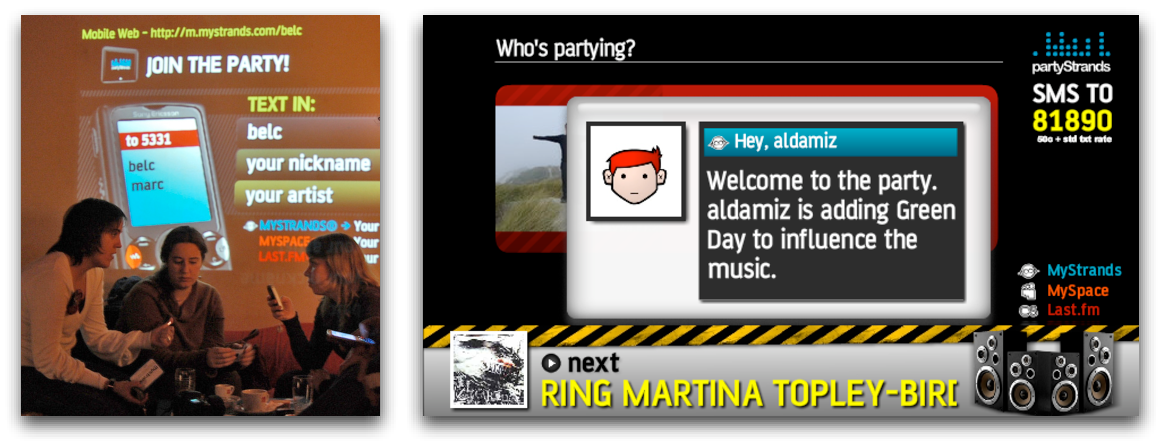
\epsfig{file=img/fig5_1, width=\textwidth}
\caption{PartyStrands in action.}
\label{fig:partystrands}
\end{figure}

% paragraph partystrands (end)

%\paragraph{The Smart Party \cite{Eustice08}} % (fold)
%\label{par:the_smart_party} ``allows user devices to seamlessly and transparently detect, configure, and interact socially in physical locations.'' Does not use domain knowledge, and does not explain how user profiles are created and preferences aggregated.
%% paragraph the_smart_party (end)

%Another similar application is Jukola \cite{OHara04}.

%Another most advanced application is described in \cite{Feldmeier07}, a system consisting of ``wireless sensors that are given to audience members to collect rhythm and activity information from the crowd [...] The pulses received [...] are analysed to detect activity levels and rhythmic features of the audience. These parameters are then available to be mapped to musical content and/or lighting control information. [...] The sound and lighting changes are then realised, to which the audience in turn responds, allowing the experience to build upon itself and giving the users an increased connection to the music.'' DK: Music is generated with loops UP: Nothing, just sensors. AG: what the sensor get (average basically)

%\paragraph{Adaptive Radio} % (fold)
%\label{par:adaptive_radio} uses negative preferences, which makes sense since the system is designed mainly to avoid the playing of music that is disliked by any member (to expand)
%% paragraph adaptive_radio (end)

% subsection similar_applications (end)


\subsection{Internet radios} % (fold)
\label{sub:problems_of_web_radios}

Music is the driving force of the recent transformation of Internet into a social medium. People turn to the Web not just to consume music, but to publish, discuss, share and discover music with friends \cite{McGuire05}.
Indeed social context in music adaptive systems is ``much more important than previously thought'' \cite{McEnnis07}. This preamble explains the success of \textbf{digital music services} such as MySpace, Last.fm and MusicStrands that provide hundreds of millions of users with virtual communities where to interact with other music lovers. % and music streams personalised for each individual.

Given this social demand, it is surprising to observe how online radios offer a service that is very close to old-fashioned AM/FM radios. 
Internet radios first appeared in 1994 \cite{WXYC04} with the intention to broadcast music over the net rather than over the air. 
Millions of online radio stations are available, but the \emph{listening experience} for the audience is still very limited: listeners ignore who else is connected to each station, cannot interact with each other nor request songs or influence the music played.

This has not stopped online radios from growing, with a weekly radio audience estimated in 33 million listeners in the United States \cite{Arbitron08} and a tendency to rise: while listening to AM/FM radio declined four percent, listening to online radio increased 18 percent and free streaming of online music increased 37 percent \cite{NPD05}.

The main competitors for online radios are Web-based music communities that broadcast personalised music streams to their members. 
Last.fm\,---\,the largest of these communities with 37.3 millions monthly unique visitors \cite{Lastfm09}\,---\,offers unlimited personalised channels for a monthly subscription of 3 euros. 

The difference between online radios and digital music services such as Last.fm is that online radios broadcast a fixed amount of music stations that everyone can browse and join at any moment, while in Last.fm channels are private: each members gets a personalised and unique music stream that cannot be shared with other listeners.


% \citet{Mediapost08} also reported that the Internet has surpassed radio as the preferred medium for music among youth in all countries, and that 63 percent of Web radio listeners have a profile on a social Web site, compared to an average of 24 percent.

% Figure~\ref{fig:radio-comparison} shows the main difference between conventional and online radios.
% It can be observed that although Internet radio gains in many aspect, it suffers in the aspect of sociality. 
% 
% \begin{figure}[hbtp]
% \centering \setlength{\abovecaptionskip}{3pt}
% \epsfig{file=img/radio_comparison, width=\textwidth}
% \caption{Comparison of terrestrial and Internet radio.}
% \label{fig:radio-comparison}
% \end{figure}



% section previous_work9 (end)

\section{The Web interface} % (fold)
\label{sec:innovative_features}


The basic service provided by Poolcasting Web radio is online music streaming.
Similarly to other Internet radios, visitors navigate with their Web browsers to the radio home-page (see Fig.\ref{fig:channels-list}), select one channel from the list and start listening to a continuous sequence of songs.
%
\begin{figure}[bthp]
\centering \setlength{\abovecaptionskip}{3pt}
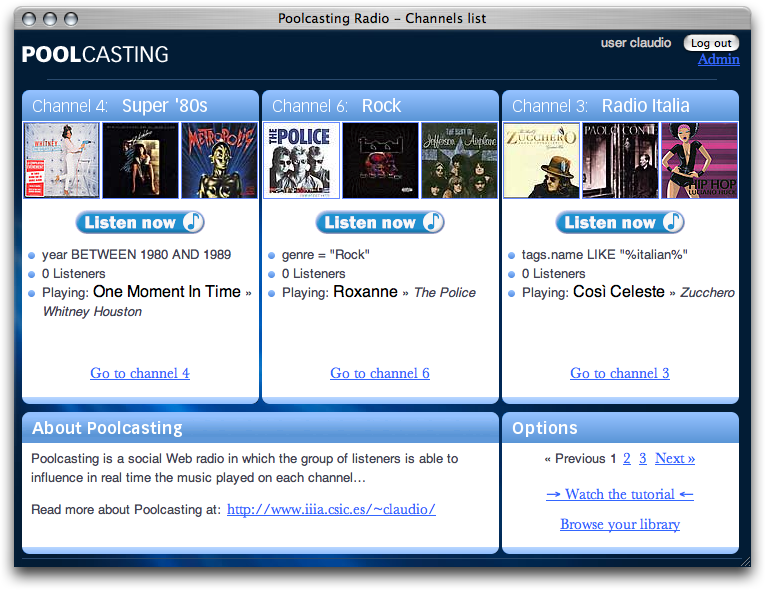
\epsfig{file=img/pwr_list, width=\textwidth}
\caption{Channels list in Poolcasting Web radio home-page.}
\label{fig:channels-list}
\end{figure}

Listening to music is very simple: users just have to click on the `Listen now' button and an appropriate streaming media player (e.g., iTunes, VLC, Winamp) opens up playing the music broadcast from that radio channel.
Another option is to navigate to the Web page of a particular channel (e.g., the `Love the '90s' channel in Fig.~\ref{fig:rock_channel}) and start the integrated Adobe Flash player to listen to music directly in the browser.
%
\begin{figure}[bthp]
\centering \setlength{\abovecaptionskip}{3pt}
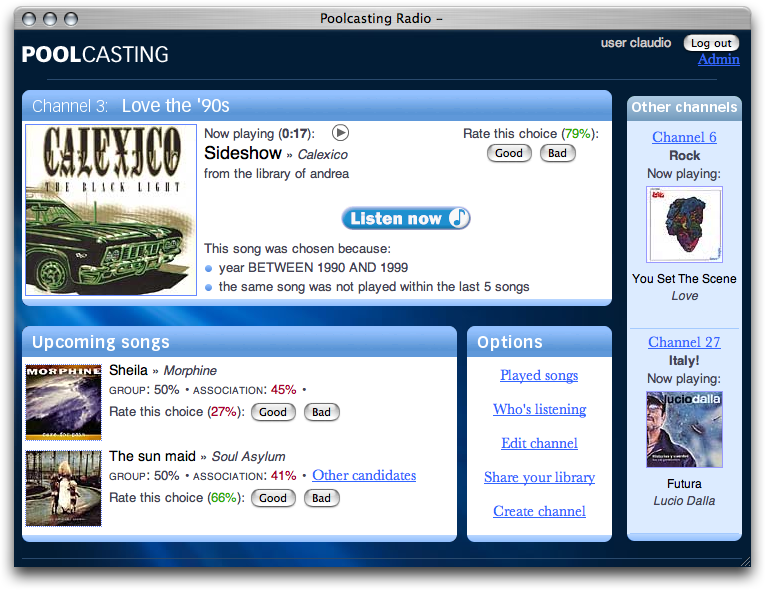
\epsfig{file=img/pwr_channel, width=\textwidth}
\caption{Web interface of a poolcasting radio channel.}
\label{fig:rock_channel}
\end{figure}
%

Tuning into a channel is a concise and intuitive process, so people who just want to passively listen to music can do so.
However, users who want to actively participate in the selection of the music played can do so swiftly as well with the different functions offered by Poolcasting Web radio.

\subsection{Sharing personal music libraries}

Internet radios typically have a large repository of songs stored on a server that some administrators continuously maintain and update to include new releases.
%Still, some listeners may find the library poor or inappropriate; for instance it may contain too many mainstream tracks, or too many obscure songs, or it may be not sufficiently updated.

Poolcasting Web radio abandons this \emph{centralised} storage model in favour of a \emph{distributed} model where the collection of music is provided by the same listeners.
The radio introduces the ability for listeners to share their personal music libraries, that is, to contribute with songs they own to the collection of music the radio can broadcast.

To share their music libraries and become active participants, users click on the `Share your library' link and indicate the path to the local folder where their personal library is stored (see Fig.~\ref{fig:share}). 
This folder has to be accessible from the network via HTTP and the music library managed with Apple iTunes.
%
\begin{figure}[bthp]
\centering \setlength{\abovecaptionskip}{3pt}
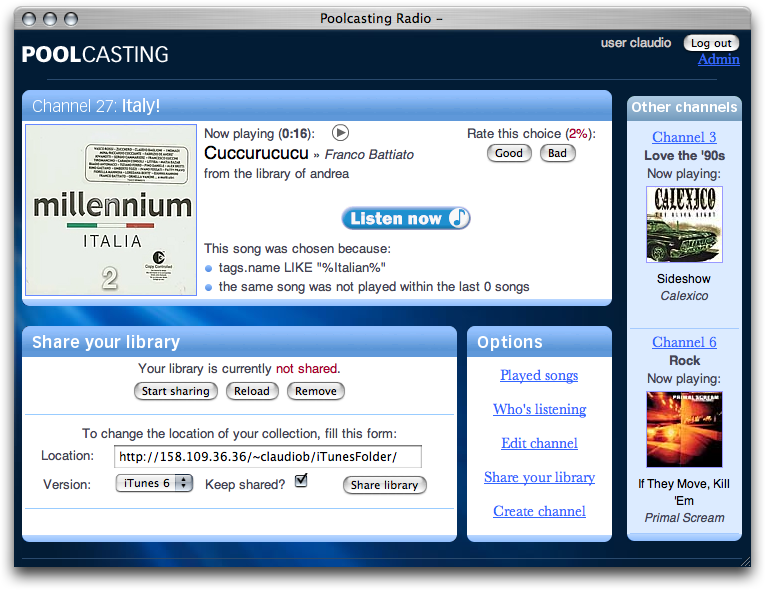
\epsfig{file=img/pwr_share, width=\textwidth}
\caption{Sharing personal music libraries in Poolcasting Web radio.}
\label{fig:share}
\end{figure}
%
After a listener has clicked on `Share library', the system connects to the specified folder and uploads the `iTunes Library.xml' file which contains the list of included songs and listening behaviour data.

Each song in the list is matched against two music recognition Web services.
The first service is OpenStrands, a Web API provided by MusicStrands that returns a unique ID for more than six million songs, fixing wrongly spelled song titles or artist names (e.g., `Obladi Oblada' instead of `Ob-la-di Ob-la-da' or `Mum' instead of `M\'{u}m'). 
Additionally, each song is matched against the Last.fm database through the Last.fm Web API. 
This double check ensures a high identification rate and is also useful to retrieve further information such as the album cover, genre, year and tags of each song.

The `iTunes Library.xml' file also contains the listening habits of each participant; as explained in Sect.~\ref{sec:estimating_individual_preferences} play counts and user ratings are used to automatically infer the preference $i(U,X)$ of each listener for each song.

Each shared library, together with the estimated preferences, is considered by the radio as a new case base.
As described in Sect.~\ref{sec:the_case_based_reasoning_selection_process}, poolcasting holds a collection of case bases, one for each participant;
each case refers to a song, its performing artist and its preference. Figure~\ref{fig:casebases} illustrates with an example how two personal libraries are represented as case bases: songs are matched against OpenStrands Web service, their song and artist IDs are used to univocally identify each song $X$ and artist $a(X)$ while the individual preferences $i(U,X)$ are assessed from the analysis of play counts and user ratings.
%
\begin{figure}[bthp]
\centering \setlength{\abovecaptionskip}{3pt}
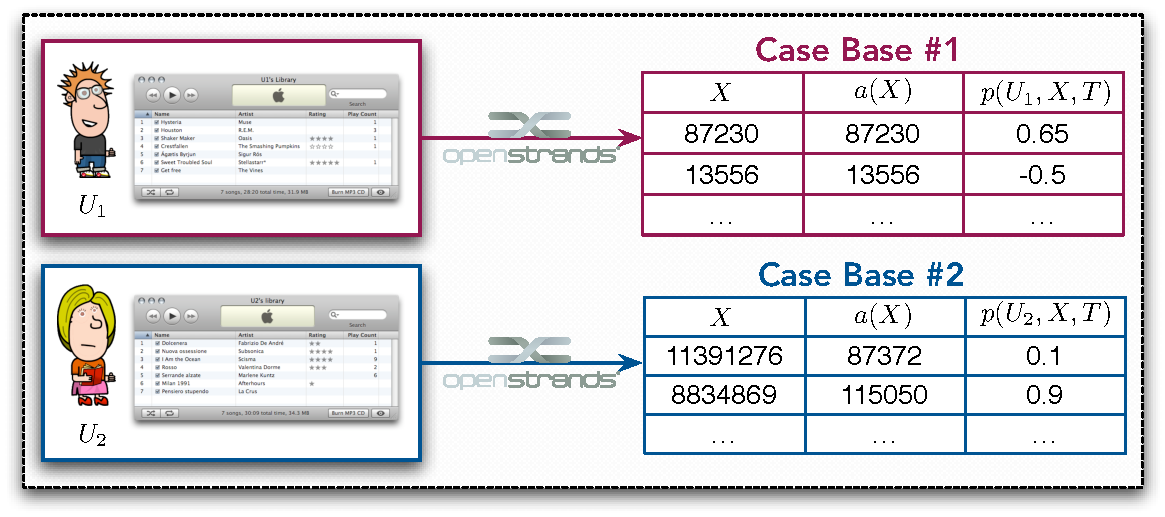
\epsfig{file=img/fig5_5, width=\textwidth}
\caption{From personal libraries to case bases.}
\label{fig:casebases}
\end{figure}

The last piece of information that is collected from the iTunes index file is the location of each song on the hard disk of the library owner.
With this information, the radio can access any shared song as long as the corresponding library owner is connected to the network.

%Having retrieved the index files that describe the content of each shared iTunes library, the system knows the exact location of each song in the hard disk of each participant and, as long as the participants are online, can upload to the radio server any song from any shared library and play them on any radio channel.

% paragraph the_library_parser_ (end)

% The collection of songs shared by all the listeners is called the \textbf{music pool} and will be indicated with $\mathcal{C}$, while the set of all the radio listeners will be indicated with $\mathcal{U}$. Since audience can change over time (people may leave or abandon a channel at every moment), I will also use the notations $\mathcal{C}_T \subseteq \mathcal{C}$ and $\mathcal{U}_T \subseteq \mathcal{U}$ to denote the set of available songs and current listeners of a channel at a given `time' $T \in \mathbb{N}^+$, where time refers to the number of songs played so far in the channel (e.g., $\mathcal{U}_5$ indicates the people listening to the fifth song broadcast on the channel and $\mathcal{C}_5$ indicates the set of songs available to be played at that moment).

The collection of songs shared by all the listeners is called the \textbf{music pool}.
There are several advantages of having a music pool distributed among multiple listeners rather than a centralised radio repository on a server.
Firstly, a distributed collection is more dynamic: when participants share their music libraries, the songs in their hard disks virtually enter the music pool; when one participant leaves, a portion of songs are removed; in general the music pool continuously varies over time.
Next, a distributed collection is more up-to-date: while an administrator would usually update the radio library once a week or a month, individuals add new songs to their libraries every day and these instantly enter the music pool.
A distributed collection also contains more of the longed for `audio not available elsewhere': in fact personal libraries often include songs not publicly distributed (e.g., personal audio material, uncommon records, alternative versions of known themes).
Finally, a distributed collection  contains a finer selection of songs: while a centralised library is normally a massive heterogeneous collection of albums, not filtered by any quality criteria, personal libraries usually contain themes the owner has manually selected and implicitly appreciates.

The fact that the system retrieves and broadcasts music from personal libraries raises questions about copyright issues and licensing policies.
While sharing and streaming music is not an illegal activity per se, most songs are currently published under restrictive licenses that prohibit free public diffusion.
In order to avoid incurring in legal issues, the radio has two options.
The first consists in limiting the service to songs published under non-restrictive licenses such as Creative Commons \cite{CreativeCommons04} that do not forbid sharing or broadcasting.
The second option is to pay the appropriate fee to the national collecting societies in charge of handing out the money to the corresponding music right holders. 
In Spain this monthly fee ranges between 56.26 and 450.11 euros depending on the nature of the service (commercial or not) and on the number of listeners \cite{Sgae06}. %http://www.sgae.es/tipology/est/item/es/1025_291.html]
% when the personal libraries contain DRM-protected songs, these are not broadcast. 

\subsection{Creating radio channels}

Online Web radios typically provide a large but fixed set of channels. Live365, for instance, offers about 6,000 radio stations, ranging from Christmas music to 80's Metal.
Some of these may have no listeners at all; still the administrators will have spent time in their creation and money in songs acquisition, storage space and bandwidth.
Large as the number of channels can be, some listeners may still be unsatisfied for they will not find \emph{the} channel that best fits their taste.

Poolcasting Web radio abandons this authoritarian model and introduces the ability for listeners to create their own channels. 
Participants can browse the list of active channels and, if they do not find the one they like, create a new one by clicking on `Create a channel' (see Fig.~\ref{fig:create}) and indicating its name, description and \textbf{channel pool}, that is, the subset of songs allowed to play. 
The channel pool is defined in terms of genres, tags and years, for instance ``Jazz from 1967'' or ``Italian Electronic Dance''.
Every newly created channel automatically appears in the home-page and is programmed with music that fulfils the specified restrictions.
\begin{figure}[bthp]
\centering \setlength{\abovecaptionskip}{3pt}
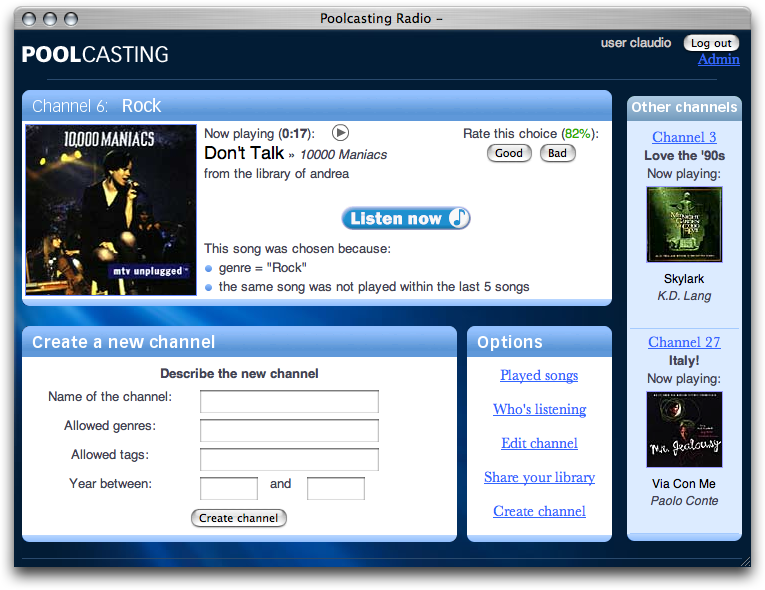
\epsfig{file=img/pwr_create, width=\textwidth}
\caption{Creating radio channels in Poolcasting Web radio.}
\label{fig:create}
\end{figure}

%The music that is allowed to play on each channel depends on two factors: the definition of the channel and the songs that are currently shared on the radio.

%Channels can be defined to play only songs within a particular period, genre or `tag'; for instance a party only plays Dance music or a radio station only plays old Italian themes. The songs that match this filter are called the \textbf{content} of the channel and are indicated with $\mathcal{C}$.


\subsection{Expressing musical preferences} % (fold)
\label{sub:expressing_musical_preferences}

Poolcasting Web radio is similar to common radios in that songs cannot be skipped: they are played from the beginning to the end, one after the other in a continuous stream.
The distinguishing feature is that listeners can express their preferences for every song in the radio and their preferences influence the music scheduled next on each channel.

Listeners can express their musical preferences in two ways. 
The first method is implicit: by sharing one's personal music library.
Shared libraries are viewed by the system as case bases and the individual listening habits data contained (play counts and ratings) are automatically analysed to assess individual preferences $i(U,X)$.

The second method is explicit: providing feedback through the `Good' and `Bad' buttons that appear close to each song (see Fig.~\ref{fig:rock_channel}).
The explicit feedback provided by a participant for a song is indicated by the function $e: \mathcal{U} \times \mathcal{C} \times \mathbb{N}^+ \to [-1,1]$.
The actual value of $e(U,X,T)$ depends on the most recent preference stated through the Web interface at time $T$, as follows:
\begin{itemize}
 \item $e(U,X,T) = 0.5$ if $U$ has clicked once on `Good' for song $X$; 
 \item $e(U,X,T) = 1$ if $U$ has clicked twice or more on `Good' for song $X$; 
 \item $e(U,X,T) = -0.5$ if $U$ has clicked once on `Bad' for song $X$; 
 \item $e(U,X,T) = -1$ if $U$ has clicked twice or more on `Bad' for song $X$; 
 \item $e(U,X,T) = 0$ if $U$ % has not clicked on any button or 
has first clicked on one button and then on the other one for song $X$.
\end{itemize}

% TO ADD: The selection has been limited to two buttons for simplicity!

As defined in \eqref{eq:preference_model2}, the \textbf{individual preference} $p: \mathcal{U} \times \mathcal{C} \times \mathbb{N}^+ \to [-1,1]$ of a person for a song corresponds to the last feedback $e(U,X,T)$ provided, falling back to the preference $i(U,X)$ assessed by the listening habits if no feedback 
was ever provided.
% \begin{equation}
% \label{eq:preference_model}
% p(U,X,T) = 
% \begin{cases}
% i(U,X) & \text{if $e(U,X,T)$ is undefined}\\
% e(U,X,T) & \text{otherwise.}
% \end{cases}
% \end{equation}

% The function $p(U,X,T)$ indicates how much a listener $U$ would like song $X$ to be selected to play next on the channel at time $T$. Calculating this function for all the current listeners with respect to all the songs in the retrieved set brings valuable knowledge about which songs are more or less adapt to satisfy the channel audience.

\subsection{Additional features} % (fold)
\label{sub:additional_features}

Another feature that characterises Poolcasting Web radio is the presence of a live chat integrated in every channel, which makes the members of the audience aware of who else is listening to the same channel (see Fig.~\ref{fig:chat}).
%
\begin{figure}[bthp]
\centering \setlength{\abovecaptionskip}{3pt}
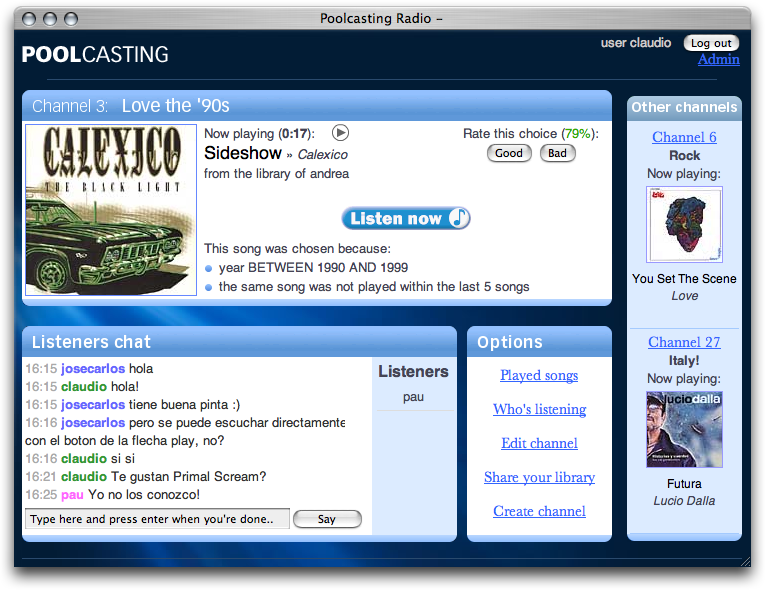
\epsfig{file=img/pwr_chat, width=\textwidth}
\caption{Discussing with other poolcasting listeners.}
\label{fig:chat}
\end{figure}

Poolcasting Web radio also includes an administrative interface that enables a super user to control the various aspects of the radio, from starting and stopping channels to checking the available domain knowledge (musical associations and preferences), from listing the active participants to removing unused channels (see Fig.~\ref{fig:admin}).
%
\begin{figure}[bthp]
\centering \setlength{\abovecaptionskip}{3pt}
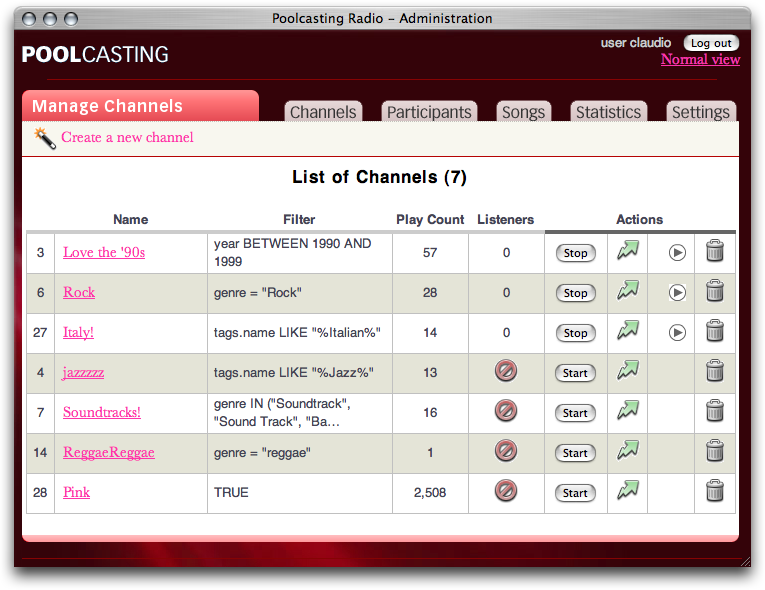
\epsfig{file=img/pwr_admin, width=\textwidth}
\caption{Administration panel of Poolcasting Web radio.}
\label{fig:admin}
\end{figure}

A feature that is common to AM/FM radios but is not present in Poolcasting Web radio is the chance for the audience to directly \emph{request} specific songs.
The reason is that Poolcasting Web radio longs to deliver a musical sequence with a certain musical continuity from song to song (\ref{p:smoothness}).
Accepting direct requests would force the radio to play any kind of music on each channel without guaranteeing smooth transitions from each song to the next.
Direct music requests would also raise issues of fairness in case the system were faced with multiple simultaneous requests and would only be able to please one.
Additionally, online radios that accept requests are regulated by more expensive licensing fees. % collecting societies \cite{Sgae06}.



% subsection additional_features (end)

%Notice that Poolcasting does not immediately and surely play a requested song, for this would infringe most Web radios copyright policies. 
\section{Automated music programming} % (fold)
%\section{The life cycle of a radio channel}
\label{sub:the_reuse_process4}

The music that is played on each channel of the radio is automatically determined by an independent poolcasting CBR process.
The whole radio is initially idle until the first participant joins the system and creates a new channel. At this point, the system spawns a poolcasting process that will determine in real time which songs will be played on that channel.

The songs available to be played are the songs shared by the current participants (music pool), although only a subset % $\mathcal{C}$ 
(channel pool) is allowed to play on each channel (e.g., only `Rock' songs in a channel defined as `genre = Rock').
%
From the channel pool, the system selects at random the first two songs $H_1$ and $H_2$.
The radio connects via HTTP to the personal music libraries where these songs are stored, uploads them to the server and starts broadcasting the first song $H_1$ over the Internet.
Then, the process selects which song $H_3$ to play next; this is accomplished by means of the CBR process introduced in Sect.~\ref{sec:the_case_based_reasoning_selection_process}.

First (retrieve process) the system identifies in the case bases a set of $\kappa = 15$ songs that have not been recently played and that form a smooth musical transition after $H_2$, the previous song in the queue.
These constitute the retrieved set of songs that are good candidates to become $H_3$.

Next (reuse process) the system ranks the candidate set combining the preferences of the listeners with the satisfaction-weighted without misery strategy detailed in Sect.~\ref{sec:social-choice-problem}.
The result is a ranked set where the top ranked candidate is the song that best addresses the goals of customisation and fairness according to the individual preferences stored in the case bases.

The top ranked song is shown in the channel Web page and, if participants do not review their preferences, is played on the channel right after $H_2$.
However at this point (revise process) listeners have the chance to browse the list of candidates and express feedback for each of these songs.

Figure~\ref{fig:pwr_candidates} illustrates the situation of a channel where the first song $H_1$ is playing (`Sideshow' by Calexico), the second song $H_2$ is on the server ready to be played (`Another Invented Disease' by Manic Street Preachers) and `Infidelity (Only You)' (Skunk Anansie) is the best candidate to become $H_3$.
By clicking on `Other candidates', listeners can revise the whole retrieved set and update their preferences for every candidate. 
If a candidate receives a large positive feedback, its group preference degree can surpass that of `Infidelity (Only You)' making that song become the new top ranked candidate.
%
\begin{figure}[tbhp]
\centering \setlength{\abovecaptionskip}{3pt}
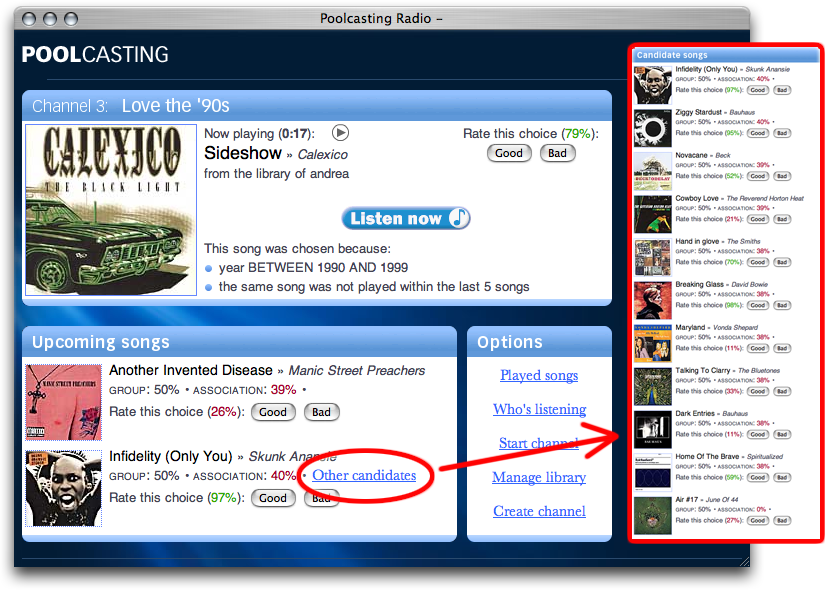
\epsfig{file=img/pwr_candidates, width=\textwidth}
\caption{Retrieved set for a Poolcasting Web radio channel.}
\label{fig:pwr_candidates}
\end{figure}

The revise process continues until the currently playing song $H_1$ terminates. At that moment, the song $H_2$ starts being streamed, the current top ranked candidate is determined as $H_3$ and uploaded to the server to be played next, and the CBR process starts again to select the song $H_4$.

As illustrated in Fig.~\ref{fig:select_and_deliver}, the music played on each channel is therefore automatically selected `one song in advance'.
While the first song $H_1$ is playing, the second song $H_2$ is uploaded to the server and poolcasting determines a set of good candidates to become $H_3$.
The implicit preferences of the audience determine the best ranked song while participants can use the `Good' and `Bad' buttons in the Web interface to revise in real time these preferences.
When $H_1$ ends, song $H_2$ starts, the best candidate to become $H_3$ is uploaded to the server and the process starts again to select $H_4$.
%
\begin{figure}[bthp]
\centering \setlength{\abovecaptionskip}{3pt}
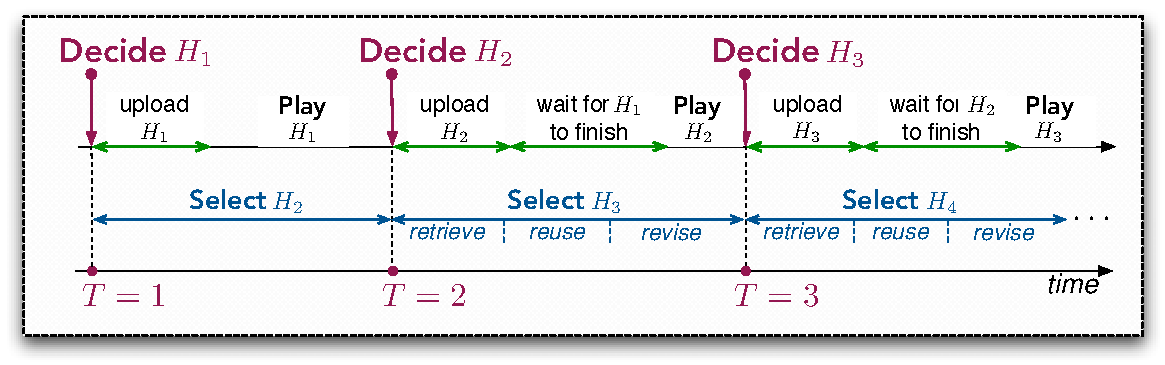
\epsfig{file=img/fig5_10, width=\textwidth}
\caption{A song is playing, the next one uploaded and the next one selected.}
\label{fig:select_and_deliver}
\end{figure}

The reason why poolcasting runs one song in advance is to guarantee an uninterrupted stream of music on each channel.
Whenever a song is playing, the next song has to be already on the server to avoid gaps in the broadcast.
Uploading a song from a personal library and encoding its audio into a proper streaming format require a certain amount of time.
Running the process one song in advance provides the duration of an entire song (typically 3 to 4 minutes) to complete these tasks and also grants enough time to `fall back' to another candidate is the top ranked one suddenly becomes unreachable (e.g., the library where it is contained disconnects from the network).

Music is broadcast from a centralised server rather than from personal libraries in order to guarantee a stable audio quality over time.
If songs were streamed directly from personal libraries (e.g. with a distributed peer-to-peer architecture), the bandwidth of the broadcaster would represent a bottleneck for the audio quality of the stream.
Moreover, if the broadcaster suddenly disconnected from the system, the stream would suffer an undesired break, which is avoided by streaming music from a centralised server after having uploading songs into a temporary buffer.

% ALSO: IF A SONG IS SUDDENLY UNAVAILABLE, THE NEXT IN QUEUE CAN BE LOADED

% The complete CBR process that at every step schedules a new song to play on a channel is illustrated in Fig.~\ref{fig:cbr_process} and is explained hereafter.
% [ NOTE: This figure is wrong: audience goes to pool of songs, and case base also contains preferences, and revise is not clear]
% \begin{figure}[hbtp]
% \centering \setlength{\abovecaptionskip}{3pt}
% \epsfig{file=img/cbr_radio_process, width=\textwidth}
% \caption{The Case-Based Reasoning selection process.}
% \label{fig:cbr_process}
% \end{figure}
% 
% \begin{figure}[hbtp]
% \centering \setlength{\abovecaptionskip}{3pt}
% \epsfig{file=img/iterative_cbr, width=\textwidth}
% \caption{The Case-Based Reasoning selection process.}
% \label{fig:iter_cbr_process}
% \end{figure}
% 
 


% Yet, poolcasting gives the audience the chance to revise their preferences, which can cause the ranking to change.
% As explained in Sect.N, a certain time has to pass from when a song $Z$ is scheduled to when it is actually broadcast. % (namely, the duration of the two  previously scheduled songs $X$ and $Y$). 
% During this time, any listener $P$ can send via the Web interface her explicit preference towards $Z$. If this occurs, the \emph{implicit preference} $g(P,Z)$ that was stored in the Case Base of $P$ (inferred from the music library) is replaced with this new \emph{explicit evaluation} provided.
% For example, if $P$ disapproves of the scheduling of $Z$, then the implicit value of $g(P,Z)$  in the Case Base of $P$ is replaced with the explicit value $-1$.
% Next, since the Case Base has changed, the retrieved set is re-ranked to include this new value in the evaluation of the group preferences.
% This can lead to $Z$ not being the most group-preferred song anymore; in this case, the scheduled song changes to the one that maximises the group preference.
% This process (user evaluations and re-ranking) continues until song $Y$ starts playing on the channel.
% Then, $Z$ is downloaded to the local buffer, and the CBR component restarts, to schedule the next song.
% 
% The generation is assisted so it's not `optimum' but continuous, in real time, and users can `tune' it before it is created (after the ranking).
% 
% 
% The revise process is meant for the audience to update their preferences for the retrieved items.
% If a member expresses a new explicit preference $e(U,X,T)$ for an item, then poolcasting recalculates its group preference.
% This can result in the a different ranking of the retrieved set and in a new item being the candidate with the highest group fairness degree $g(X,T)$.
% 
% When the revise process finishes, poolcasting delivers the best ranked item to the audience, adds it to the list of delivered items as $H_T$ and updates the satisfaction degree $q(U,T)$ of each participant $U \in \mathcal{U}_T$ , so that the least satisfied members will be favoured for the selection of the next items.
% 
% \paragraph{AAAI} % (fold)
% \label{par:aaai6}
% Participants can also use the Web interface to rate whether they liked or not songs they have been listening to on a channel. 
% When a user sends a feedback about a song, her preference model is updated with her new explicit evaluation. 
% For example, if $P$ listens to a new song $Y$ and sends a positive feedback, the system stores the information that $P$ has a high preference for $Y$.
% As a result, the next Reuse processes will be influenced by this new value, and will eventually schedule other songs associated with $Y$ while $P$ is listening. % to that channel.
% % paragraph aaai6 (end)
%
% subsection the_revise_process3 (end)

%Poolcasting Web radio continuously checks \emph{who} is listening to each channel and selects music based on their musical preferences. In this way, listeners do not have to `jump' from one channel to the other looking for music they like. Poolcasting \emph{adapts} the content of each channel for its listeners and not vice versa.


\section{Implementation}\label{subsection:architecture}

%As part of the research, the Poolcasting Web radio architecture described in this chapter has actually been implemented.
%
The development of Poolcasting Web radio took about one year and % and was completed in October 2007. 
its final architecture is illustrated in Fig.~\ref{fig:poolcasting-architecture}.
%
\begin{figure}[bthp]
\centering \setlength{\abovecaptionskip}{3pt}
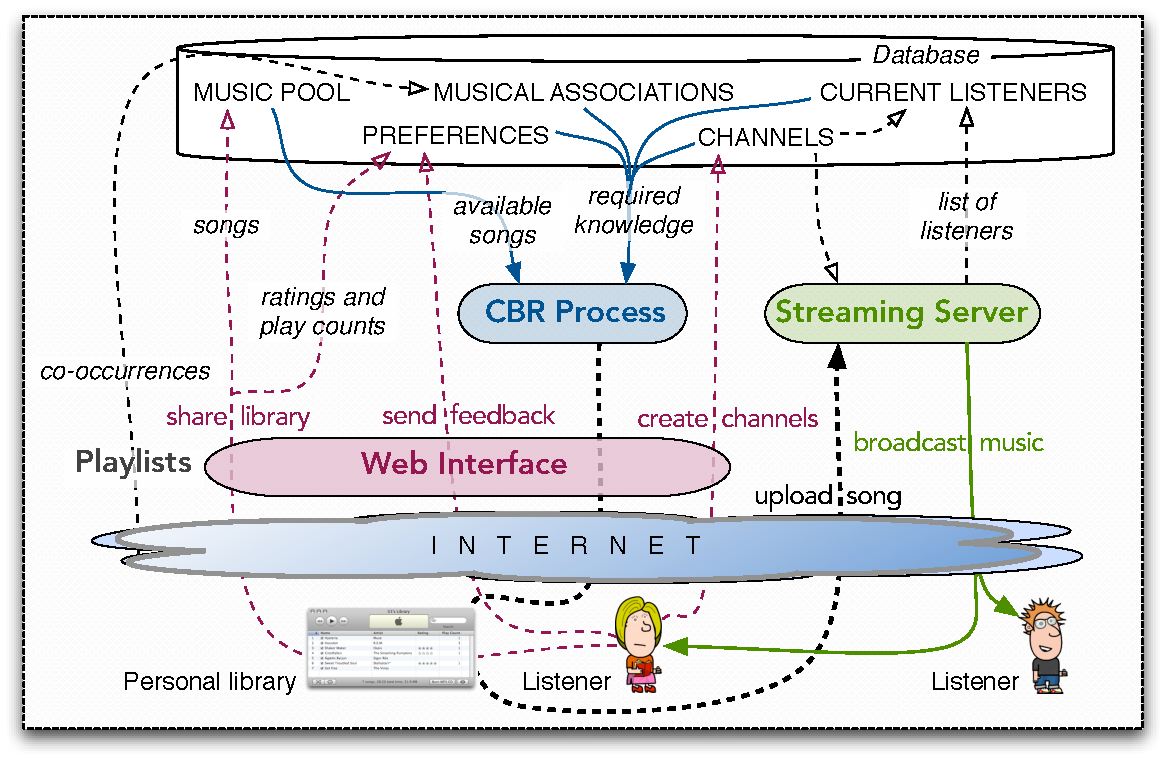
\epsfig{file=img/fig5_11, width=\textwidth}
\caption{Architecture of Poolcasting Web radio.}
\label{fig:poolcasting-architecture}
\end{figure}

The radio is idle until a participant creates a channel through the Web interface.
When this occurs, the streaming server opens a new Internet stream for the channel and a CBR process is started to fill the stream with music.
The CBR process continuously checks in the database which songs are available (music pool), which ones fit the current channel (channel pool), how well each song would go after the last song played (musical associations) and how each of the current listeners like each song (individual preferences).
Having gathered this required knowledge, the process returns the ranked set of candidates that participants can revise by sending `Good'/`Bad' feedback through the Web interface.

When the best candidate is determined, the radio connects via HTTP to the library where the song is contained, uploads the audio file to the server and passes its content to the streaming server as an uncompressed audio signal.
The streaming server encodes the audio into a proper streaming format (either 
MP3 or OggVorbis) that is later broadcast to the connected listeners.

The streaming server also maintains a list of the IP addresses of the listeners of each channel; channels that have not had any listener are automatically disabled after some time, in order to save bandwidth.

The entire framework has been running on a Mac Pro server equipped with two Dual-Core Intel Xeon CPUs at 2.66 GHz and 6 GB of memory. %, providing a private radio service to the IIIA.
%
All the components of the radio have been developed with open source software: \textsf{Ruby on Rails} for the Web interface, \textsf{Apache} for the Web server, \textsf{MySQL} for the database, \textsf{Ruby} for the CBR process, \textsf{liquidsoap} \cite{Baelde08} to manage the music queue and the stream generator, \textsf{icecast} for the streaming server.




% subsection technical_details (end)



% This section works but may be superfluous



\section{Summary} % (fold)
\label{sec:conclusions8}

This chapter has described a new Web radio framework that delivers group-customised music channels, offering an innovative social radio experience.

Poolcasting Web radio combines bottom-up and top-down approaches: users can express their musical preferences while the actual choice of music played is taken by a CBR process that iteratively checks which songs are available and who is listening and selects the songs that most satisfy the current audience.

The advantage of the radio architecture is that user interaction allows the system to model the musical preferences of each listener and exploit them to customise the content of the channels.
Feedback expressed in terms of `Good'/`Bad' preferences offers a direct overview of the listeners' preferences;
in addition, the radio can work without any user interaction by exploiting the implicit knowledge contained in the personal music libraries shared by the participants.

Poolcasting Web radio merges the distributed nature of online radios with the personalised nature of music recommenders, thus offering a groundbreaking Internet service that can satisfy the needs of several Web music listeners.



% section conclusions8 (end)
% chapter poolcasting_web_radio2 (end)

\chapter{Experiments and evaluation} % (fold)
\label{cha:evaluation}
\songquote{Everybody makes mistakes,\\
But I feel alright when I come undone}{LCD Soundsystem, 2005} 
% Here comes two of you,
% which one will you chose?
% One is black, one is blue.
% I'm beginning to see the light - Velvet Goldmine

% Not all good things come to an end now it is only a chosen few

%And do you think it's so easy to find
%Somebody who is just your kind
%Oh, it might take you a little time
% Pulp - happy endings



% All the people are dancing
% and they're having such fun
% I wish it could happen to me
% after hours - velvet u

\section{Working with a real Web radio}

This chapter is divided in two parts.
The first two sections describe the experience of ten actual users with Poolcasting Web radio: which channels they created, which songs they shared, which impressions they perceived.
The rest of the chapter reports of experiments to evaluate how poolcasting can deliver radio channels that address the goals of customisation and fairness.
A particular attention is dedicated to measure how the size and the musical homogeneity of the audience can affect the group satisfaction.

\subsection{The active audience} % (fold)
\label{sub:the_audience2}

An implementation of Poolcasting Web radio has been running for one year on a Web server located in the internal network of the Institut d'Investigaci\'{o} en Inte\lgem ig\`{e}ncia Artificial (IIIA-CSIC).
The radio has been showcased in different research institutes, % (IIIA-CSIC, Queen Mary University, University College of London), to
music-related companies % (MusicStrands, Last.fm) 
and international conferences \cite{Baccigalupo07c,Baccigalupo07e,Baccigalupo07f};
% The radio requires users to authenticate; 
at each presentation the audience was asked to join and evaluate the system. A total of 29 persons accepted, ten of which have connected to the radio more than once. 
These `active' users are male and 30 years old in average; five are Italian, four are Spanish and one is English.
% subsection the_audience2 (end)

\subsection{The music pool} % (fold)
\label{sub:the_music_pool}

Eight of the ten participants agreed to share on the radio the songs contained in their personal music libraries.
The total number of shared songs was 60,202. 
Matching these titles against OpenStrands and Last.fm Web services and discarding duplicates reduced the size of the music pool to 24,763 songs.

Five of the eight shared libraries were online 24 hours a day since they were stored on computers that were never switched off; the remaining three libraries were instead only available when the computers where they reside were connected to the Web.

%According to the data stored in the respective iTunes libraries, 
The most common genres for the songs in the music pool were: Rock (3,499 songs), Soundtrack (2,670), Pop (1,609), Alternative \& Punk (1,156), Electronic (614), Alternative Rock (560) and Indie (504). 
Most songs were published in 2005 (1,642 songs), while the average year of publication was 1999.
%
%According to the data retrieved from 
Matching the music pool against Last.fm Web service revealed the following tags as the most common: rock \& pop (9,138 songs), alternative (1,402), international (1,178), hard rock (529), r\&b (520).

% subsection the_music_pool (end)

\subsection{Listening habits} % (fold)
\label{sub:listening_habits}

The listening habits data stored in the shared libraries revealed that most participants had never played or rated the songs contained in their libraries.

Only 4,564 of the 24,263 songs (18.4\%) had ever been played by their owners in iTunes, while only 358 songs (1.4\%) had been rated. % with a certain number of `stars'.
The average play count for the 4,828 songs that had ever been played or rated was 1.8 times while the average rating was 3.3 stars.

These data interestingly point out how people may hold large music libraries in their hard disks and still play and rate only a small amount of songs, leaving most of their music collection untouched.

%select count(*) from archives where itunes_count is not null and library_id in (1,2,3,5,7,13,10,12,15) and song_id is not null;

% subsection listening_habits (end)

\subsection{Observations} % (fold)
\label{sub:observations12}

Although the radio was presented to about 100 persons, only ten became active participants.
Informal interviews to those who did not join the radio revealed two main reasons. 
Some people were unfamiliar with online radios and were not interested in trying a new one. Others appreciated the idea of a social Web radio but did not have a music library managed with Apple iTunes, so could not actively participate. % to poolcasting.

The ten active users showed a noticeable interest for Poolcasting Web radio, to which they connected day after day.
The number of shared songs was quite large compared to the number of listeners (in average 2,476 tracks per user), which enabled people to frequently discover unknown music.

A negative characteristic related to the active users was the low rate of played and rated songs in their personal libraries, which allowed poolcasting to build only partial models of their music profiles, restricted to a few songs and artists. 
The feedback provided through the `Good' and `Bad' buttons on the Web interface resulted very important to refine these music profiles over time.


% subsection observations12 (end)


\section{Variety and smoothness} % (fold)
\label{sub:active_channels}

Fifteen distinct channels were created by the ten active users of the radio. 
Most channels were defined as single-genre (e.g., `Rock' channel); others using periods (e.g. `Music from the Eighties'); others combining genres and tags (e.g., a `Soundtracks' channel playing tracks tagged as `Soundtrack', `Sound track', `Banda Sonora' or `BSO'\footnote{`BSO' stands for `Banda Sonora Original', `Original Soundtrack' in Spanish.}).
Although participants could alter the definition of a channel after its creation, this function was barely used.

\subsection{Variety} % (fold)
\label{sub:variety2}

The variety of the music played on each channel (\ref{p:variety}) was achieved by setting the repetition parameters to $\eta = 50$ and $\zeta = 5$ (see Sect.~\ref{sec:the_case_based_reasoning_selection_process}): every song could be repeated on the same channel only after 50 other songs, while songs by the same artist had to be separated by at least 5 songs.
These values were meant to avoid short-term repetition of the same music.

A problem reported by some listeners was that channels would sometimes repeat the same \emph{sequence} of songs in consecutive days.
For instance, whenever `Romeo Had Juliette' (Lou Reed) played in the `Rock' channel, it was always followed by `The Wait' (The Pretenders).

The reason for this behaviour is that `The Wait' is the top associated song with `Romeo Had Juliette' in the music pool according to the knowledge in the data set of playlists.
This means that, in the retrieve process, `The Wait' always ranks as the best candidate to follow `Romeo Had Juliette' and, in the reuse process, is the song selected to play next, unless the audience explicitly states a negative feedback.

To avoid this unpleasant behaviour, the requirement for variety was strengthened, forbidding that any \emph{pair of consecutive songs} could be repeated two times in a row in the same channel.
The song `Romeo Had Juliette', for instance, would be followed by `The Wait' (the top associated song) on its first appearance in the `Rock' channel, 
while it would be followed by `The Same Situation' (Joni Mitchell)\,---\,the second top associated track\,---\,on its second occurrence, and so on.
This enabled the radio to achieve both short-term and long-term variety.

\subsection{Smoothness} % (fold)
\label{sub:smoothness2}

Poolcasting Web radio reuses the musical associations extracted from the analysis of playlists (see Chap.~\ref{cha:smoothness}) to address the requirement of smoothness (\ref{p:smoothness}). 

An example of smooth musical sequence delivered on the `Rock' channel was: `Pretty Noose' (Soundgarden), `Bullet with Butterfly Wings' (Smashing Pumpkins), `Kool Thing' (Sonic Youth), `MFC' (Pearl Jam), `Medication' (Queens of the Stone Age).
This sequence shows a certain continuity since all these songs revolve around the U.S. Indie Rock sound of the Nineties and go well together both for acoustic and cultural reasons.

Imposing smooth transitions from song to song comes at a price: the influence of the listeners is narrowed to decide only among a few candidates. As a result, a channel can take a long time to adapt content to the audience.

An example was reported by an active user of the `Rock' channel who had to wait for the duration of four songs (about fifteen minutes) before listening to an Electronic Rock track, akin to his musical profile.
The reason was that, because of the smoothness requirement, poolcasting could not `jump' directly from one style to another but had to pass through a series of intermediate tracks before reaching an Electronic Rock track.

To avoid this behaviour, the smoothness requirement in Poolcasting Web radio was relaxed to include randomly chosen tracks in the retrieved set as well as songs that were musically related to the previous one.
Specifically, the retrieve process was modified to retrieve the top 10 candidates from the list of associated tracks and the last 5 candidates at random from the channel pool.
If the listeners ranked any of these songs better than the rest, that song would be played next, even without being the most associated with the last one.
%
The Electronic Rock lover of the previous example, for instance, could in this way browse the retrieved set and pick the random candidate which was most akin to his musical taste, rapidly bending the music towards a more Electronic style.

With this approach, faster transitions could occur from a sub-genre to another when persons with different musical taste were present in a channel.

% subsection active_channels (end)

\subsection{Observations} % (fold)
\label{sub:subjective_evaluation}

Other characteristics that the audience particularly appreciated or objected were revealed in a series of interviews to the radio listeners.

% PAU
One participant found among the greatest qualities of Poolcasting Web radio ``the idea of taking music out of personal libraries to new listeners''. This was seen as a great way to get to know new composers and songs. Another quality was the ``direct participation of the listener, which makes it a social radio''.
The main drawbacks observed were that ``a channel can rapidly become overcrowded, negatively affecting individual satisfaction'' and also the fact that musical preferences assessed from iTunes libraries can be wrong when the users are not ``careful with their content, which can badly affect the quality of the transmission''.

% NEAL
A different participant replied that the best aspects of the radio were ``the interface, the streaming audio quality and the social aspect of the radio, even though I did not have the chance to fully delve into this''. The worst aspect found was ``having to wait for songs I did not like to finish''. The participant also commented that ``this kind of radio would work best in a shared office, where people are not just interacting \emph{online} as they listen to the music''.
%+ very few channels..

% MANU
A third participant rated positively the ``comfortable interface'', while was worried about the long time that had to pass before the radio could learn individual musical preferences. 
In his opinion, Poolcasting Web radio can make listeners ``quite satisfied'' but not ``totally satisfied'', something that is positively ``compensated by getting to discover new music that you are probably going to like''.

%-Interfaz muy cómoda y agradable de ver.
%-La sensación que me queda es que hay que estar mucho tiempo escuchando la radio para que pueda aprender tus preferencias.
%-Creo que la radio sólo puede llegar a tenerte "lo suficientemente satisfecho", pero no "totalmente satisfecho". De todas maneras, esto ya es suficiente, cuando la recompensa es conocer canciones nuevas de grupos que seguro que te van a gustar.
%Detalles menores:
%-Cada vez que la canción cambia es necesario volver a pulsar el botón de play para escuchar la música.
%-Sólo por azar se da uno cuenta que hacer dos veces click en bad no es lo mismo que bad. ¿Por qué no poner directamente "very bad" y "very good"?
% Dudas:
%-¿Poolcasting utiliza la librería del usuario para aprender? ¿O era algo que has hecho después?


% CLAUDIO
A fourth participant appreciated the fact of being able to ``rediscover songs from the bottom of my music library, that I did not remember having''.
\citet{Voida06} already investigated the satisfaction given by this ``rediscovery'' experience which is correlated to the increasingly large music libraries that characterise several iTunes users.

The main lesson learnt is that the listeners of Poolcasting Web radio implicitly accept a social compromise. When they join a channel, they are aware they will not possibly like every song played, yet they will have the chance to easily discover new music preferred by other listeners, with whom they can interact and discuss.
This social component would not exist if they were to play music directly from their personal digital players or from other Internet radios.

% subsection observations94 (end)

% 
% 
% 
% \paragraph{Example of customisation.} % (fold)
% \label{par:example_of_customisation_}
% Some experiments. The first one is the following: I set up the same channel with the same library, but in one case I have no user modelling (all neutral), in the other I have it, and I observe how things change (using a deterministic choice, always the first candidate).
% 
% without: Pretty Noose (Soundgarden) -> Bullet with Butterfly Wings (Smashing Pumpkins) -> Kool Thing (Sonic Youth) -> (Drawing) Rings.. (Super Furry Animals) -> Everybody's Got Something.. (The Beatles) -> MFC (Pearl Jam) -> Medication (Queens of the Stone Age)
% 
% with personalisation (and I like electronic apart from Rock): Pretty Noose (Soundgarden) -> Elderly Woman.. (Pearl Jam) -> Kool Thing (Sonic Youth) -> Seventeen (Ladytron) -> Tribulations (LCD Soundsystem) -> 23 (Blonde Redhead) -> Objects of my affection (Peter Bjorn \& John).
% % paragraph example_of_customisation_ (end)
% 
% % subsection subjective_evaluation (end)
% 
% [TO DO: Experiments with the SYSTEM, such as each channel requires this amount of memory, on a G4 only 4 channels can run simultaneously, etc.]
% 
% % section experiments_with_the_radio (end)


\section{Group customisation and fairness} % (fold)
\label{sec:evaluation_of_this_technique}

The previous section reported on experiences of real users of Poolcasting Web radio and on the way in which radio channels achieve a level of variety (\ref{p:variety}) and smoothness (\ref{p:smoothness}) that is appropriate for the audience.
%
The rest of the chapter evaluates whether the poolcasting technique can achieve the goals of customisation (\ref{p:customisation}) and fairness (\ref{p:fairness}) on groups of different sizes and musical homogeneity.

To obtain objective results, independent of the particular music profiles of the ten active users, the evaluation is run in a simulated environment with a set of artificially created profiles.

% Each profile is generated with random music preferences, that is, each user is designed to like some songs and dislike other ones at random. 
% More precisely, the preference degrees $i(U,X)$ of each artificial user $U$ for each song $X$ have been generated as a uniformly random distribution of numbers in $[-1,1]$, as illustrated in Fig.~\ref{fig:unif_dist}
% %
% \begin{figure}[bthp]
% \centering \setlength{\abovecaptionskip}{3pt}
% \epsfig{file=img/unif_dist, width=\textwidth}
% \caption{Uniform distribution of preference degrees [CHANGE].}
% \label{fig:unif_dist}
% \end{figure}
% % x <- sort(runif(1000))*2-1; plot(x,dnorm(x=x,sd=0.5),type="l",ylim=c(0,1))
 
%The evaluation is run by creating a radio channel with a certain number of `fake' listeners, running the CBR process that chooses which songs to play according to their preferences and finally analysing whether poolcasting has achieved its purpose of adapting the music to the audience (\ref{p:customisation}) and having all the user satisfied over time (\ref{p:fairness}).

\subsection{Random music profiles} % (fold)
\label{sub:initial_configuration}


The first experiment evaluates the performance of poolcasting in a radio channel with five participants.
Each person is simulated by an artificial music profile that describes which songs a participant likes and dislikes.
Precisely, five music profiles are generated \emph{randomly}, that is, assigning a random number in $[-1,1]$ to the individual preference $i(U,X)$ of each participant $U \in \mathcal{U}$ for each song $X \in \mathcal{C}$.

This is intended to emulate a sort of worst case scenario where five members of a channel do not share any particular musical affinity: one may like some Pop and Rock songs and detest Heavy Metal tracks, another may like Jazz and Rock and dislike Pop, and so on.

The five participants all join the same radio channel, defined with no filter: all the available music is allowed to play, from any genre, year or tag.
The channel is started, and the first song is played at random from the available ones.
%
All the successive songs are selected by the poolcasting CBR technique described in Sect.~\ref{sec:the_case_based_reasoning_selection_process}, with the parameters initially set to $\kappa = 15$ (size of the retrieved set), $\iota = 0.4$ (initial satisfaction), $\chi = 0.8$ (satisfaction decay) and $\mu = -0.75$ (misery threshold).

Whenever a new song is played, the values of two functions are registered for every participant $U$:
\begin{itemize}
 \item $h(U,T)$, that is, how much $U$ likes the song played; and
 \item $q(U,T)$, that is, how satisfied $U$ is for the songs played so far.
\end{itemize}

After $25$ songs, the channel is stopped and the registered values are analysed.
In order to obtain significant results, the whole process (creating a channel, playing 25 songs, collecting results) is replicated 20 times with different initial random songs and music profiles and the analysis is performed on the average values of $h(U,T)$ and $q(U,T)$ through all the iterations.

This experiment is meant to evaluate whether poolcasting can fairly satisfy a group of five listeners characterised by random music profiles.
This can be considered as a sort of worst case scenario since in the real world listeners of the same radio channel typically share some musical affinity.

\subsection{Results} % (fold)
\label{sub:initial_results}

Figure~\ref{fig:default} shows the result of this evaluation.
Each line in the graph corresponds to one of the five participants. 
The plot on the left shows the individual preferences $h(U,T)$ of each participant for each of the 25 songs played; the plot on the right indicates their satisfaction degrees $q(U,T)$ after each song.
%
\begin{figure}[bthp]
\centering \setlength{\abovecaptionskip}{3pt}
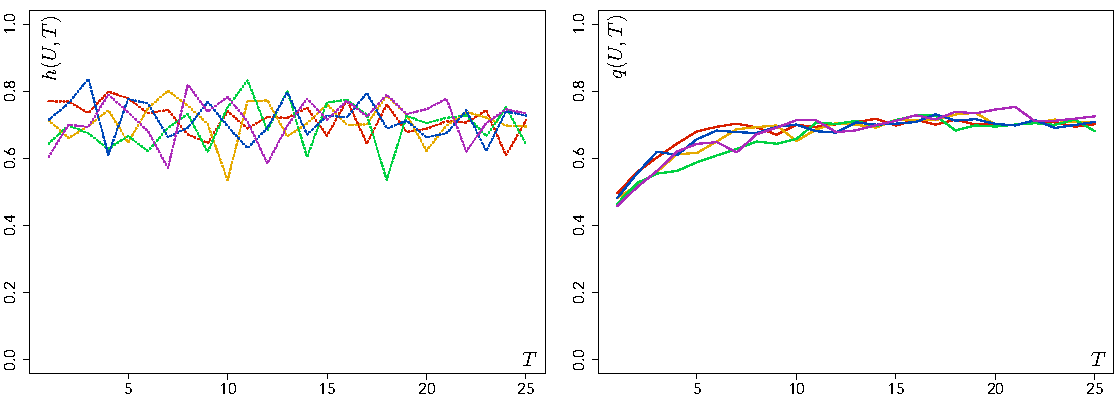
\epsfig{file=img/fig6_1, width=\textwidth}
\caption{Individual preferences and satisfaction degrees of five participants listening to the same channel for the duration of 25 songs.}
\label{fig:default}
\end{figure}

With regard to customisation, the results look positive.
The whole audience likes every song, %more or less 
with an average individual preference of
% means = apply(preferences, c(1,2), mean, na.rm=TRUE)
$\overline{h(U,T)} = 0.72$.
%
Lower spikes in Fig.~\ref{fig:default} (left) indicate songs that a participant did not particularly like; even in these occasions the preference $h(U,T)$ never falls below a value of $0.5$.
Moreover, lower spikes are immediately followed by high values, demonstrating the power of poolcasting in rewarding participants who did not like some of the recently played songs.

The impact of this balanced strategy over individual satisfactions is illustrated in Fig.~\ref{fig:default} (right).
All the lines are quite close and stable over time, indicating that poolcasting achieves fairness by keeping every participant similarly satisfied in the long run.

% The standard deviation of $h(U,T)$ for all the songs and participants is as low as $0.05$.

The difference between the most and the least satisfied listener is small: $q(U,T)$ has an average standard deviation of $0.04$ which means that a reasonable degree of fairness is achieved.
The satisfaction of the group as a whole is quite high for this kind of worst case scenario, in fact the average satisfaction degree over the 25 songs played equals $\overline{q(U,T)} = 0.68$.


\section{Discordant listeners} % (fold)
\label{sec:discordant_listeners}
 
The previous section has evaluated poolcasting on a group of listeners with random individual preferences. 
In that case, poolcasting was able to deliver a group-customised sequence of songs to satisfy the entire audience.

This section considers a different situation in which five participants are split into two purely antagonist groups: the music that three users prefer, the other two dislike, and vice versa. No song exists that the entire audience likes.

The rationale of this experiment is to prove whether poolcasting can achieve fairness with discordant listeners, determining a sequence of songs that, in the long run, can match the preferences of all the participants.
Again, this is a sort of worst case scenario: in the real world, listeners of the same radio channels typically share musical affinities for some songs.

For the sake of this experiment, five artificial profiles are created to simulate five participants split into two discordant groups.
Three users are assigned with random \emph{positive} preferences $i(U,X)$ for half of the available songs and with random \emph{negative} preferences for the remaining half; the opposite occurs for the other two users.

Figure~\ref{fig:random} (left) illustrates this distribution on a sample set of ten songs: the users labelled as 1, 2 and 3 only like the last five songs, while the users labelled as 4 and 5 only like the first five songs.
By comparison, Fig.~\ref{fig:random} (right) represents the scenario previously evaluated in Sect.~\ref{sec:evaluation_of_this_technique} where individual preferences were independently assigned among listeners.
%
\begin{figure}[bthp]
\centering \setlength{\abovecaptionskip}{3pt}
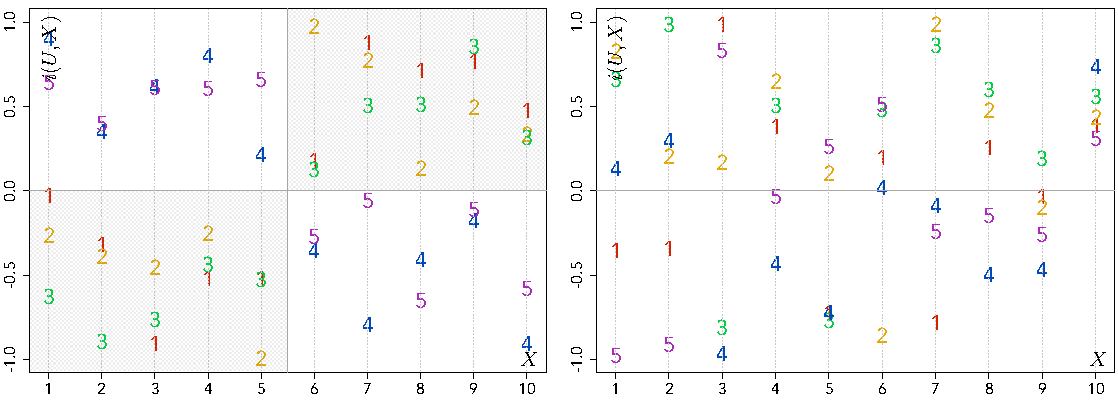
\epsfig{file=img/fig6_2, width=\textwidth}
\caption{Sample individual preferences of five participants whose profiles belong to two discordant groups (left) or are independent (right).}
\label{fig:random}
\end{figure}

The evaluation is run as in Sect.~\ref{sec:evaluation_of_this_technique}, having the channel playing $25$ songs, repeating the process $20$ times with different initial songs, and observing the values of $h(U,T)$ and $q(U,T)$ at each iteration. 
%The only difference is in the creation of the artificial user profiles.  Rather than simply having random preference degrees, in this case a majority of the audience (three listeners) has random \emph{positive} preferences for half of the music pool and random \emph{negative} preferences for the rest, while the opposite occurs for the minority (two listeners).

\subsection{Results} % (fold)
\label{sub:results73}

The results of the evaluation are shown in Fig.~\ref{fig:fair_1}: 
the plot on the left marks the individual preferences $h(U,T)$ for the songs played; the plot on the right indicates the satisfaction degrees $q(U,T)$ of the five participants.
%
\begin{figure}[bthp]
\centering \setlength{\abovecaptionskip}{3pt}
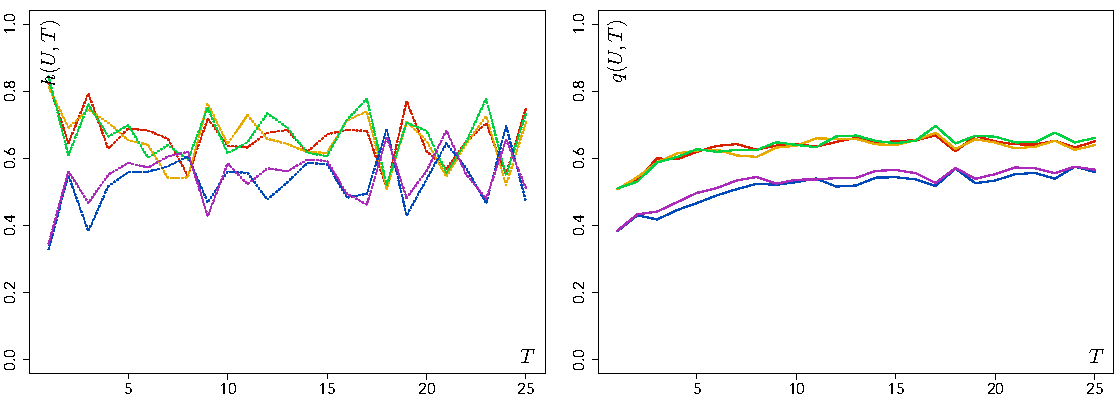
\epsfig{file=img/fig6_3, width=\textwidth}
\caption{Individual preferences and satisfaction degrees of five participants split in two groups with discordant music profiles.}
\label{fig:fair_1}
\end{figure}

%\subsection{Observations} % (fold)
%\label{sub:observations9}

The first observation is that the two groups can be clearly identified in the graphs: most played songs are preferred by three participants who, as a consequence, have a higher satisfaction degree.

Still, the difference between the two groups is not very large and whenever a song preferred by the majority is played, a song preferred by the minority is played soon after. 
The songs played at position 8, 18, 21 and 24, for instance, are preferred by the minority more than by the majority. %, as shown in Fig.~\ref{fig:fair_1} (left).
Moreover, every song played, although preferred by one of the two antagonist groups, has been selected to be reasonably acceptable by the members of the other group, albeit to a lesser degree.

The motivation for this balanced outcome is the satisfaction-weighted aggregation strategy presented in Sect.~\ref{sec:social-choice-problem} that combines individual preferences rewarding less satisfied listeners.
In this case, two participants are generally less satisfied than the other three so once in a while poolcasting delivers one of their favourite songs, to achieve fairness.

Thanks to this approach, the distance between the satisfaction degrees of the groups does not increase over time, as shown in Fig.~\ref{fig:fair_1} (right). 
This result is notably positive considering that actual radio channels do not typically have an audience split into two purely antagonist groups.

\subsection{The importance of memory} % (fold)
\label{sub:comparison_with_plurality_voting}

In the previous experiment, a certain degree of fairness was achieved thanks to the satisfaction-weighted aggregation strategy that holds memory of previous outcomes to determine which items to deliver next.

To prove that this strategy is the responsible for the positive results obtained, an equivalent experiment is run under the same conditions but using a different aggregation strategy, with no memory of past decisions.

The experiment is run with the same audience of two discordant groups but preferences are here combined with a simpler approach, selecting at each step the song that has \emph{in average} the highest preference, independently of the previous songs played. No memory of past satisfaction is kept.

The results of this experiment are shown in Fig.~\ref{fig:fair_2} which illustrates the average individual preferences (left) and satisfaction degrees (right) of the five participants for the songs played.
%
\begin{figure}[bthp]
\centering \setlength{\abovecaptionskip}{3pt}
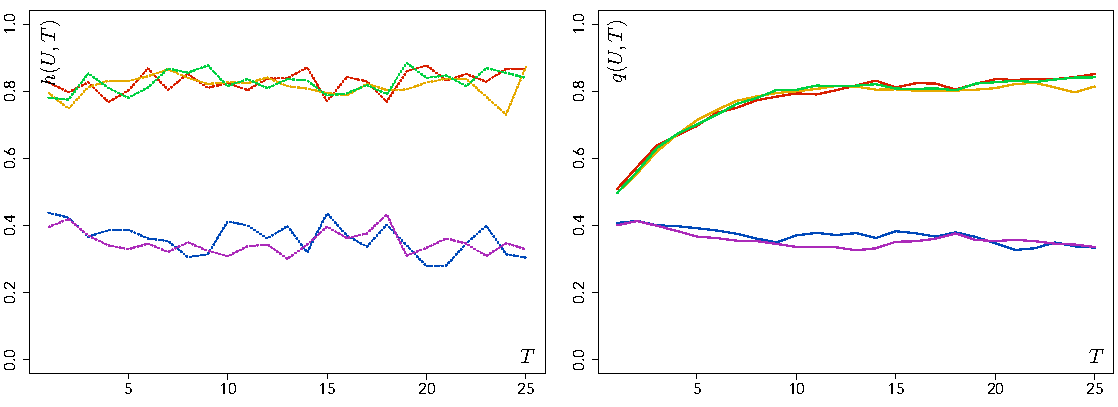
\epsfig{file=img/fig6_4, width=\textwidth}
\caption{Individual preferences and satisfaction degrees of five discordant participants when songs are selected without memory.}
\label{fig:fair_2}
\end{figure}

As can be observed in Fig.~\ref{fig:fair_2} (left), in this case the radio channel plays only songs that three participants (the majority) prefer more than the remaining two (the minority).
As a consequence, three members of the audience are more and more satisfied as time goes by, while the remaining two members are less and less satisfied, as shown in Fig.~\ref{fig:fair_2} (right).

The lesson learnt is that, without memory of past elections, fairness can only be achieved punctually, satisfying at each moment only the current majority.
The satisfaction-weighted aggregation strategy that characterises poolcasting, on the other hand, can fairly satisfy the entire audience over time, playing songs that both the majority and the minority like to a certain extent.

% subsection observations9 (end)

% subsection fairness (end)

\section{Concordant listeners} % (fold)
\label{sub:concordance}

The next experiment is meant to evaluate the performance of poolcasting in the case members of the audience share some affinity with respect to their music profiles.
While the previous sections focused on worst-case scenarios made of random or antagonist participants, this section considers a more common situation in which different listeners of the same radio channel like the same kind of music.

In this case, profiles are not generated independently one from the other, but with a certain concordance.
Precisely, for every song $X \in \mathcal{C}$ in the music pool, the  preferences $i(U,X)$ of the five participant are generated as random numbers limited to a particular sub-range of $[-1,1]$ of diameter $\vartheta \in [0,2]$, that is:
\begin{equation*}
        \max_{U \in \mathcal{U}}\,i(U,X) - \min_{U \in \mathcal{U}}\,i(U,X) \leqslant \vartheta \,\; \forall X \in \mathcal{C}\,.
\end{equation*}

The smaller the value of $\vartheta$, the closer the preferences of different participants for the same song, the stronger the affinity between music profiles. 
This distribution of music profiles is illustrated in Fig.~\ref{fig:bump} on a sample set of ten songs.
%
\begin{figure}[bthp]
\centering \setlength{\abovecaptionskip}{3pt}
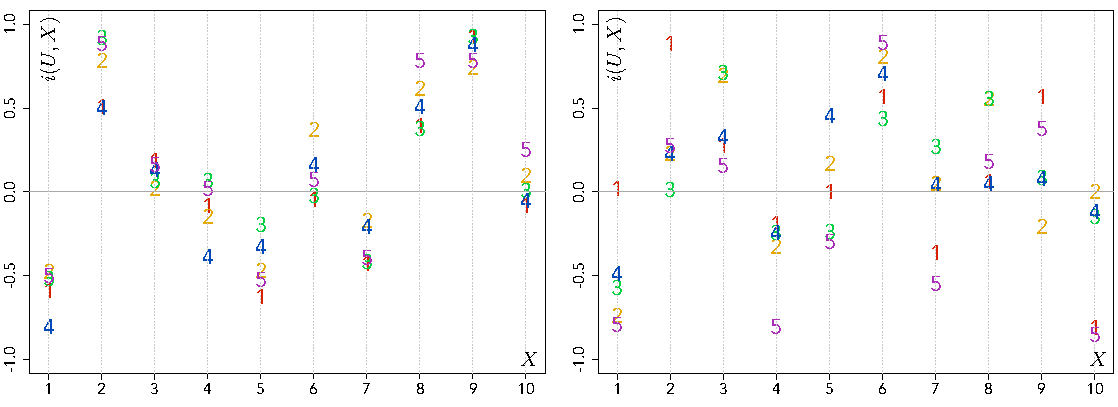
\epsfig{file=img/fig6_5, width=\textwidth}
\caption{Sample individual preferences of five participants whose profiles share an affinity of $\vartheta = 0.5$ (left) or $\vartheta = 1$ (right).}
\label{fig:bump}
\end{figure}

Figure~\ref{fig:bump} (left) represents the situation where $\vartheta = 0.5$; in this case all the individual preferences $i(U,X)$ for the first song are restricted to negative values in $[-0.9,-0.4]$, all the preferences for the second song are positive with values in $[0.4,0.9]$, all the preferences for the third song are medium with values in $[-0.2,0.3]$, and so on.
Figure~\ref{fig:bump} (right) illustrates the situation with a larger diameter $\vartheta = 1$; in this case the affinity is less evident. Note that when $\vartheta = 2$, the situation is identical to Fig.~\ref{fig:random} (right).

The evaluation of the experiment is run as in Sect.~\ref{sec:evaluation_of_this_technique}, with five participants listening to $25$ songs played on a channel, repeating the process $20$ times with different initial songs, and observing the values of $h(U,T)$ and $q(U,T)$ at each iteration.

\subsection{Results} % (fold)
\label{sub:results44}

Figure~\ref{fig:bump2} (left) shows the results when $\vartheta = 0.5$, that is, when participants have a quite strong affinity in musical taste. 
Compared to Fig.~\ref{fig:default} (right) (audience with no musical homogeneity), the results improve with respect to both the average individual preference (increased to $\overline{h(U,T)} = 0.86$) and the variance among different users (the standard deviation decreases to $0.02$).
%
\begin{figure}[bthp]
\centering \setlength{\abovecaptionskip}{3pt}
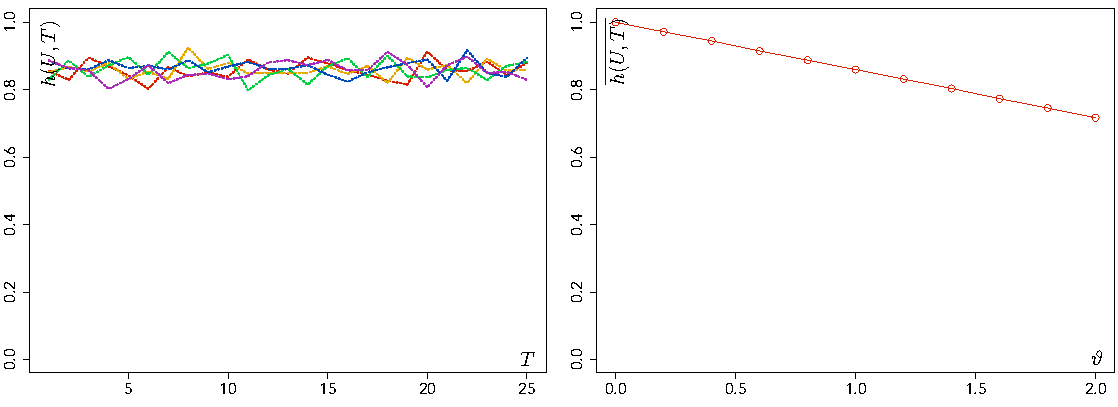
\epsfig{file=img/fig6_6, width=\textwidth}
\caption{Individual preferences for songs played when $\vartheta = 0.5$ (left) and correlation between affinity degree and average preferences (right).}
\label{fig:bump2}
\end{figure}

The relationship between group homogeneity and satisfaction is illustrated in Fig.~\ref{fig:bump2} (right), which shows how poolcasting is better able to deliver songs the audience strongly likes when the value of $\vartheta$ is small.
In the real world, a group of people listening to the same radio channel is expected to present some homogeneity in their musical taste, in which case the performance of poolcasting improves noticeably.

% subsection group_affinity (end)


\section{Scalability} % (fold)
\label{sub:scalability}

The next experiment evaluates the impact of the size of the audience over the group satisfaction.
The previous sections have only considered channels with five listeners; this section investigates whether adapting content for less or more people can affect the performance of poolcasting.

%Intuitively, adapting content for a few users should be simpler than adapting content for many users, especially when they have different preferences. This hypothesis is tested hereafter.

The evaluation is run using two new sets of artificial listeners: the first contains only two user profiles while the second simulates a group of twenty people. 
As in Sect.\ref{sec:evaluation_of_this_technique}, profiles are generated assigning random values in $[-1,1]$ to the individual preference $i(U,X)$ of each person for each song.
A channel is run for the duration of $25$ songs, the process repeated $20$ times and the satisfaction degrees $q(U,T)$ are analysed.

\subsection{Results} % (fold)
\label{sub:results345}

Figure~\ref{fig:size} shows the satisfaction degrees of the participants in a group of size 2 (left) and size 20 (right). 

Compared to the group of size 5 represented in Fig.~\ref{fig:default} (right), the satisfaction degrees are higher in Fig.~\ref{fig:size} (left) and lower in Fig.~\ref{fig:size} (right).
In other words, poolcasting has it easier to adapt content for smaller groups than for larger groups. This makes sense since the more the listeners, the more the music preferences to fulfil, and the harder to satisfy the entire audience.
Specifically, the average satisfaction degree decreases from
$\overline{q(U,T)} = 0.84$ with size 2, to $\overline{q(U,T)} = 0.72$ with size 5, to $\overline{q(U,T)} = 0.61$ with size 20.
%
\begin{figure}[bthp]
\centering \setlength{\abovecaptionskip}{3pt}
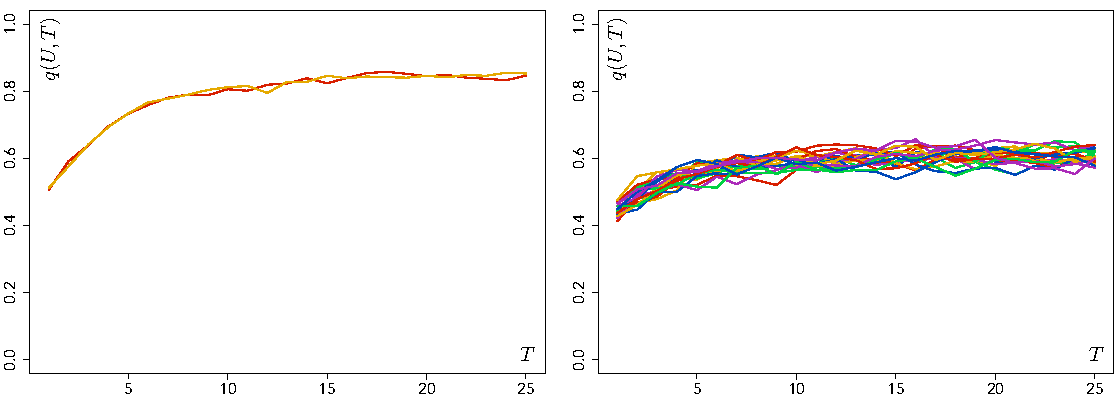
\epsfig{file=img/fig6_8, width=\textwidth}
\caption{Satisfaction degrees for a channel with 2 participants (left) or 20 listeners (right).}
\label{fig:size}
\end{figure}

More interesting, though, is that the variance between participants remains small even when the size of the group grows.
The lines plotted in Fig.~\ref{fig:size} (right) are all very close and stable over time, meaning that poolcasting is able to keep a good balance of the satisfactions of all the listeners in the long run.

Although one might conclude from this experiment that poolcasting can only be applied to radio channels with a small audience, this conclusion is not correct for a series of reasons.

Firstly, this section has focused only on a worst case scenario where all the listeners have random music preferences. 
In the real world, members of the same channel typically share some musical affinity, which makes it easier to find songs that satisfy multiple listeners at the same time.
As a consequence, group satisfaction is not always as badly affected by the group size as illustrated in Fig.~\ref{fig:size} (right).


Secondly, the experiment has been run on a channel with no filters, playing songs from every genre, tag or period. 
However most online radio stations restrict the music played to a specific set of songs (e.g. a `Rock' channel) to attract a public with a certain homogeneity in musical taste. 
As observed in Sect.~\ref{sub:concordance}, the stronger the affinity in the music profiles of the participants, the higher the satisfaction degree that poolcasting can provide, even for large groups.

%Thirdly, participants are free to join or leave a channel at different moments and, most importantly, to create new channels if they do not like the music played on existing ones (see Sect.~\ref{sec:innovative_features}). If a channel becomes too populated and a group-customised musical sequence cannot be supplied, part of the audience can move to a newly created channel (e.g., a second `Rock' channel) where poolcasting will be able to deliver songs better customised for their profiles.

Lastly, populated channels can benefit the listeners in terms of music discovery.
A listener $U$ connected to a channel with a large audience is more exposed to unknown music, played because of the preferences of other participants. 
Even though unknown songs will not match the music profiles of $U$, causing a decrease in the satisfaction degree $q(U,T)$, the chance of discovering new music is seen as a positive trade off by many listeners.

% All the participants can easily reach a satisfaction of 100\% by listening to music \emph{on their own}, selected by hand from their personal libraries, but in this way they would miss out the social component of the radio. A radio channel with a large audience, on the other hand, offers them a sequence of group-customised songs, of which some they already know and like, and others they get to discover.

The advantage of poolcasting is that, even when the audience is very large, fairness is achieved keeping the satisfaction of all the listeners balanced in the long run.

%[ TO DO: Worst case scenario shows poolcasting can maintain certain levels of performance even in a worst case scenario. More realistic scenarios will show better overall satisfaction, with more `affinity' among users. The experiments show that scalability is very correlated with group affinity, so as the channel audience grows there may be situations where affinity in audience groups will suggest to split channels.]

% subsection observations10 (end)

% subsection scalability (end)

\section{Other parameters} % (fold)
\label{sec:other_parameters}

The experiments in this section evaluate the impact of three other parameters of the poolcasting process over customisation and fairness. 

The first parameter is the retrieval size $\kappa$, which determines how many songs are selected in the retrieve process as `good candidates' to be played next. %, according to the properties of variety and smoothness.

The second parameter is the misery threshold $\mu$, which determines the minimum individual preference that any listener is willing to accept for any played song.

The third parameter is the initial satisfaction $\iota$, which determines the default value of $q(U,T)$ for a participant who has not yet listened to any song in the channel. 

All the experiments are performed under the conditions described in Sect.~\ref{sec:evaluation_of_this_technique}, with five artificial listeners with random music profiles.

%Another parameter that affects the outcome is the satisfaction decay $\chi$, which determines how rapidly each person forgets remote experiences. The effect of $\chi$ on the function $q(U,T)$ has already been examined in Sect.~\ref{sec:social-choice-problem}.
 

% section other_parameters (end)

\subsection{Retrieval size} % (fold)
\label{sub:retrieval_size}

The retrieval size $\kappa$, introduced in Sect.~\ref{sec:the_case_based_reasoning_selection_process}, indicates how many songs are selected in the retrieve step of the CBR process.
The larger the retrieval size $\kappa$, the more the candidate songs that are pre-selected to be played next, the higher the probability to find a candidate song the audience will like.
% This hypothesis that relates the value of $\kappa$ to the preference degrees $h(U,T)$ for the songs played is tested hereafter by running the evaluation process with different values of $\kappa$.

Figure~\ref{fig:default} (left) illustrated the outcome on individual preferences of running poolcasting with a default retrieval size of $\kappa = 15$. 
Figure~\ref{fig:retr_2} (left) evaluates the same process but with the parameter set to $\kappa = 30$. 
%
\begin{figure}[bthp]
\centering \setlength{\abovecaptionskip}{3pt}
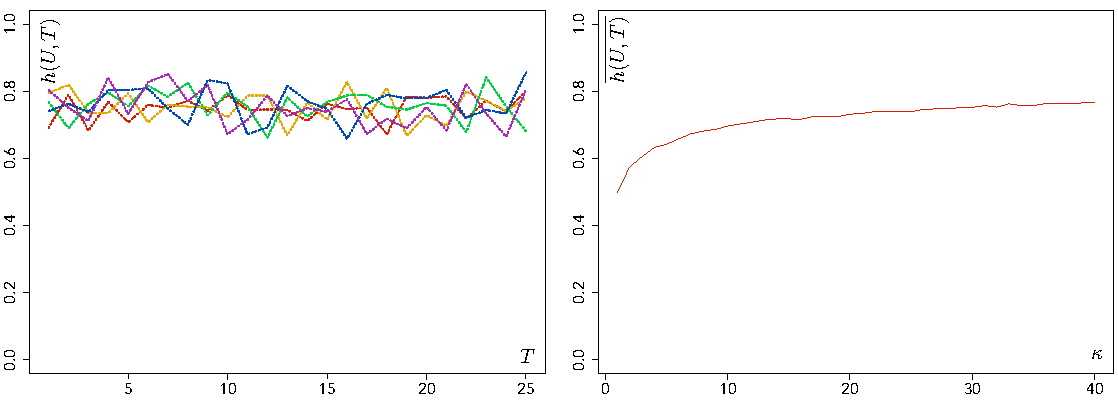
\epsfig{file=img/fig6_9, width=\textwidth}
\caption{Individual preferences for songs played when $\kappa = 30$ (left) and correlation between retrieval size and average preferences (right).}
\label{fig:retr_2}
\end{figure}

Having doubled the retrieval size, the average group preference increases but not noticeably, from $\overline{h(U,T)} = 0.72$ (with $\kappa = 15$) to 
$\overline{h(U,T)} = 0.76$ (with $\kappa = 30$).
%
Figure~\ref{fig:retr_2} (right) confirms this observation, showing the relationship between the retrieval size $\kappa$ and the average group preference $\overline{h(U,T)}$.
A clear improvement occurs in the lower range of intervals, but for values of $\kappa$ larger than 15 the average group preference remains quite stable.

For this reason, $\kappa = 15$ can be considered as a good retrieval size.
A smaller value would worsen the quality of the candidate set and, as a consequence, the quality of the played songs.
A larger value, on the other hand, would not improve much the quality and could decrease the performance of poolcasting, required to rank more candidate songs in real time.

Another good reason not to have a large retrieved set is that Poolcasting Web radio offers a Web page where listeners can send feedback for the candidate songs (see Fig.~\ref{fig:pwr_candidates}). 
If the list were too long, the audience would probably just ignore it, rather than stating a feedback which is very valuable to refine individual music profiles.

% subsection observations23 (end)

% subsection retrieval_size (end)

\subsection{Misery} % (fold)
\label{sub:misery}

Another parameter that affects the music selection process is the misery threshold $\mu \in [-1,1]$, introduced in Sect.~\ref{sub:how_we_fairly_aggregate_preferences}.
This value specifies the minimum preference degree that the audience is disposed to accept for a played song. 
For instance, if $\mu = 0$ then no song that any listener dislikes is allowed to play on the channel.
At the extreme, when $\mu = -1$ every song can be played; when $\mu = 1$ only songs that the whole public unconditionally loves can be played.

If the misery threshold is low, then every song can be played, even songs one participant detests (\emph{low minimum} individual preference) and everybody else loves (\emph{high group} preference). 
If the misery threshold is high, then only songs that no one detests (\emph{high minimum} individual preference) can be played, even if they have a \emph{low group} preference.

These two cases are illustrated in Fig.~\ref{fig:misery}, which represents the preference degrees of listeners for the songs played when the misery threshold is low ($\mu = -1$) or when the value is higher ($\mu = 0$).
The higher the threshold, the lower the average preference degree: $\overline{h(U,T)} = 0.73$ with $\mu = -1$ (left), $\overline{h(U,T)} = 0.59$ with $\mu = 0$ (right), while $\overline{h(U,T)} = 0.72$ with $\mu = -0.75$, as shown in Fig.~\ref{fig:default} (left).
%
\begin{figure}[bthp]
\centering \setlength{\abovecaptionskip}{3pt}
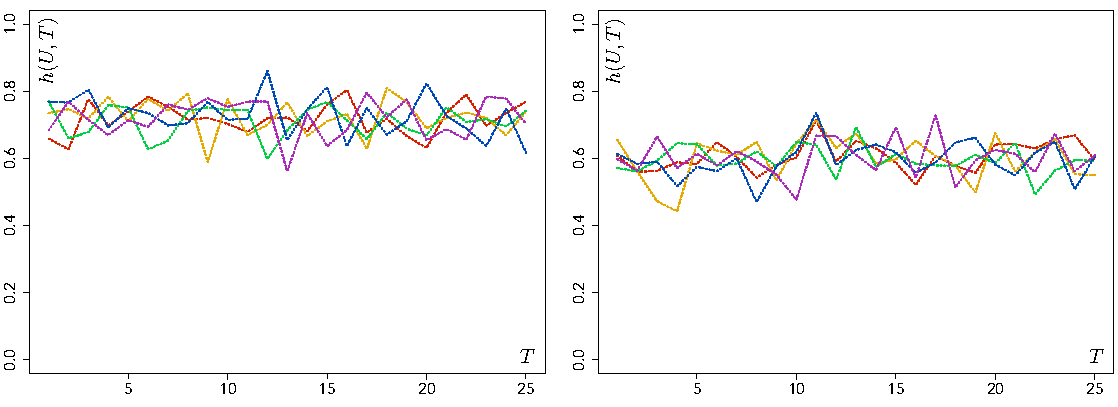
\epsfig{file=img/fig6_10, width=\textwidth}
\caption{Individual preferences for songs played when misery threshold $\mu = -1$ (left) or when $\mu = 0$ (right).}
\label{fig:misery}
\end{figure}

The lesson learnt is that the misery threshold is better kept small, since large values force poolcasting to select songs that will not bother anyone but that no one will really love either.

The threshold could as well be set to $\mu = -1$, to completely ignore the issue of misery. In fact, poolcasting listeners that do not like the songs played are already rewarded by the satisfaction-weighted aggregation.
By ignoring the issue of misery, poolcasting would make it impossible for malevolent participants to take control over the music played by strategically casting negative feedback for every song except those they would like to hear.

% subsection misery (end)


% subsection concordance (end)

% 
% 
% \subsection{Satisfaction decay} % (fold)
% \label{sub:satisfaction_decay}
% 
% Satisfaction is an emotion that decays over time, and the more recent experiences are those that affects us more. How much the remoteness of an election outcome influences the current satisfaction depends on the satisfaction decay. This graph shows how changing this factor modifies satisfaction over time; when this value equals 1, only the outcome of the last election decides the current satisfaction.
% 
% % subsection satisfaction_decay (end)
% 
% 
% 
% 
% \subsection{Weight to memory} % (fold)
% \label{sub:weight_to_memory}
% 
% This follows Experiment 4 to show how weighting the preferences of each person in relation to their preferences for previously selected items contribute to achieve fairness among different people. This graph shows how the standard deviation of satisfaction among the different persons is smaller keeping memory of past satisfactions (solid line), compared to the situations where each item is selected independently of the previous outcomes (dotted line).
% 
% Similarly to Experiment 4, individual preferences are generated with a random bimodal distribution; with three persons, two like some items and the third likes other ones; with five persons, three like some items, and the other two like other ones; and so on. The graph shows how the standard deviation of multiple satisfaction changes as the number of persons increase. Note that when the number is small (for example, 3 persons), the effect of memory is very clear, while it becomes less noticeable as the number of persons increase.
% 
% % subsection weight_to_memory (end)


\subsection{Initial satisfaction} % (fold)
\label{sub:initial_satisfaction}

The last parameter that can affect the outcome of poolcasting is the initial satisfaction $\iota \in [0,1]$, introduced in Sect.~\ref{sec:calculating_individual_satisfaction}.
This value defines the satisfaction degree of any person who has not yet listened to any song.

Figure~\ref{fig:iota} shows the effect of different values of $\iota$ on the satisfaction degrees of the participants: $\iota = 0$ (left) and $\iota = 1$ (right).
By comparison, Fig.~\ref{fig:default} (right) represented the default case where $\iota = 0.4$.
%
\begin{figure}[bthp]
\centering \setlength{\abovecaptionskip}{3pt}
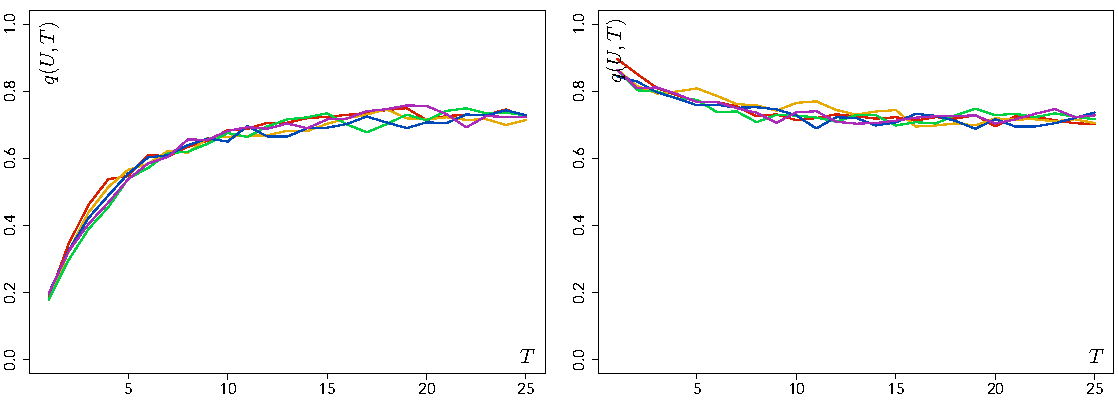
\epsfig{file=img/fig6_11, width=\textwidth}
\caption{Satisfaction degrees for songs played when participants have initial satisfaction $\iota = 0$ (left) or $\iota = 1$ (right).}
\label{fig:iota}
\end{figure}


The graph shows that the value of $\iota$ only affects individual satisfaction for the duration of the first songs.
After a while, the value is absorbed by the satisfaction decay and becomes irrelevant.
After $25$ songs, the satisfaction of the listeners is almost the same, independently of the value fixed for $\iota$.

The conclusion is that the value of $\iota$ does not affect satisfaction in the long run.
Using a default value of $\iota = 0.4$, slightly below the average, can help `boost' the importance of newcomer participants, so they can immediately listen to some songs they like when entering a channel.
This effect decays rapidly and, after a while, all the participants are treated equally independently of their initial satisfaction.

% subsection initial_satisfaction (end)

% section other_evaluations (end)





% section evaluation_of_this_technique (end)

% 
% 
% \section{The experiments with personalisation} % (fold)
% \label{sec:the_application3}
% 
% I had to create fake profiles. I matched the genres as the top tags of last.fm using \url{http://www.last.fm/group/Last.fm+Web+Services/forum/21604/_/285676}
% 
% % FAKE RATINGS FOR CLAUDIO:
% % insert into feedbacks(participant_id, candidate_id, song_id, artist_id, at_slot) select distinct 9, Null, song_id, artist_uid, Null from archives where song_id is not null and artist_uid is not null;
% % update feedbacks set degree = 2*rand()-1;
% 
% \subsection{Responsiveness} % (fold)
% \label{sub:responsiveness}
% 
% How fast the system adapts/changes?
% When user 1 enters, how long does it take to adapt? When he leaves and another one joins, what happens?
% 
% % subsection responsiveness (end)
% 
% 
% Now I repeat the same experiment, but I connect with a user to see if I influence and I get personalised sequences.
% 


% \subsection{Different influences} % (fold)
% \label{sub:different_influences}
% 
% Another evaluation is to have the channel with no filters at all and see where the music goes, in which styles, years, etc., whether it flows are stays still.
% In other words, I have a channel multi-genre and I enter with \emph{different} profiles, but ONE at the time, and see where music goes.
% 
% % subsection different_influences (end)
% 
% \subsection{Learning about personalisation over time} % (fold)
% \label{sub:learning_about_personalisation_over_time}
% 
% Explicit preferences also affect the customisation of the content for  a participant through time, at the beginning the system does not know a lot about a user, but as long as the same user continues to give ratings on the same channel, then the adaptation improves. 
% 
% another evaluation that I do with fake profiles is the following: I create these fake profiles and infer the preferences, and then I see how much satisfied the users are. now within the same channels I start giving explicit preferences, and our hypothesis is that the radio improves the customisation and the users are more satisfied. I do this and see that...
% 
% (this happens because the system has a larger knowledge)
% 
% this test I run with a channel made of a single user, has nothing to do with group customisation.
% 
% subsection learning_about_personalisation_over_time (end)

% section the_application3 (end)


% \section{Evaluation of fairness} % (fold)
% \label{sec:evaluation_of_desired_properties}
% 
% Here I should present the virtual work on the radio, with the desired properties and the parameters that affect them, and describe the problem of multi-genre channels.
% 
% \subsection{Scalability} % (fold)
% \label{sub:scalability}
% 
% How is this affected by the number of users? Number of songs?
% e.g. \emph{irony test}: I start with N songs and observe what happens when I increase/decrease the number of songs, or of users, or preferences.
% 
% If we split a large group in two, do they both increase satisfaction?
% 
% % subsection scalability (end)
% 
% \subsection{Average without misery} % (fold)
% \label{sub:average_without_misery}
% 
% Try to run the same channel but with a different aggregation method (e.g. plurality voting) and observe what happens to satisfactions.
% 
% % subsection average_without_misery (end)
% 
% \subsection{Own/other songs} % (fold)
% \label{sub:own_other_songs}
% 
% Show how often you get to listen to your own songs (fake profiles) and if this is equally distributed
% 
% % subsection own_other_songs (end)
% 
% \subsection{Individual vs. group} % (fold)
% \label{sub:individual_vs_group}
% 
% Under certain conditions, can the individual satisfaction be \emph{higher} in a group-addressed than in a personal system?
% 
% % subsection individual_vs_group (end)
% 
% 
% (explain the combination)
% 
% I do this test on the radio to see how many times the songs that is selected is selected because of song-to-song, song-.to-artustsm, a-to-a or random. once I have done this test I evaluate fairness like this., I create fake profiles with different preferences, each shanring a library, and on specific channels with different types of channel.
% \textbf{the first is channel defined with a genre}, like rock, an rpople likeing different shades of rock, and I see what happens and \textbf{how their satisfaction fluctuates} and if it's true that satisfaction enver falls below a certain threshold and what happens at this minimum satisfaction that I ever reach as I change some parameters, one of the parameter is the number of listeners. this is important because it's not the same ot satisfat a gorup of 2 or 10 persons, I try to see if 10 persons with different preferences can be satisfies, which is the maximum bnumber of people that can be satisfied, without changing the context which is defined by genre.
% 
% another test that I do is: what happens if the channel is not defined by a genre but by the period or by multiple genres or tags. if the context of the definition is very strict, then if you create a channel that is italian jazz music from the 50s and people go there, there you have strong restrictions, so if someone joins, more ore less he will be satisfied by every song played there, the selection is not very wide, while if you create a channel that is very wide, like music from the 80s, there you can have pop or rock or classical or soul, so you may start listening to pop, then people who like heavy metal join the channel, teh music should be more heavy metal,  if they leave and saoul lovers enter it hsould be more soul.
% the experiments here are to see if the music is adapted for the users. I have a channel defined as music from the 80s, withouth limitiation in terms of genres or tags, and in the bedinnging in this channel I have users who like sould and r\&b and our hypotheis is that the music that is selected from a repository that has any kind of genre available, contains more sould or r\&b music that the average. then they leave, and epople who love heavy metal enter the channel, and I want to see the number of sould and r\&b songs decrease, and metal increase. this is our hypothesis.
% and no one is very unsatisfied.
% 
% and I increase the number of users up to a limit.
% (and also I want to observe if smoothness is maintained in this transition)
% 
% 
% 
% 
% % section evaluation_of_desired_properties (end)
% 
% \section{Evaluation without a precise context} % (fold)
% \label{sec:evaluation_without_a_precise_context}
% 
% imagine now that I have in the previous situsation present at the same time, you have in a group people who like different genres, the channel as music form the 90s and 5 persons like sould r\&b and hip hop and 5 persons like rock or electronic rock or indie rock., in this situation you want to make everyone hwppy but also smoothness, I run experiement and see the sequence generated, and I don't just consider if smoothness is achieved or satisfaction is above a certain threshold, but I also look for a higher concept of smoothness, uintil now I have considered it just as song after this song, byut in this kind of sitatuion you also wanto smooth transition from a genre to the other. I ran the test and observe ...
% 
% (result)
% 
% it does not really occur wel the problem that I have is that if I just had one set, given smoothness as I have defined it then the songs tend to stay in the same area, if you are playing rock it tends to stay rock it does not navigate the whole network of artists, it tends to stay in one group becasuse there is no step to step transition from one song to the other, whay I would like to see is smyt in a more abstract senst that you go from a style to another and then go back and have smooth paths from one genre to the other. the point is that each artist is only. 
% 
% I want to see if this is true or not but I cannot because for each artists I have just one genre label, so I five songs labelled as rap and then five as rock and I don't know if in the middle there was a smooth transition from very very rap song to crossover song, and so on, this is what I would like, like a dj, if this is somethings in the middle it's good, not to jump from pure rock to pure rap. I would like to see this kind of bejhaviour in the radio. how can I do this? this is 
% 
% 
% % section evaluation_without_a_precise_context (end)
% 
% 
% % This is very unneeded! :-)
% % Evaluation may occur in labs or `in the wild'. Is there any difference? \cite{Baumann04} shows that ``there is no great difference between the two settings, and so no pressing need to implement an ecological approach to multimodal subjective similarity perception''.
% 
% 
% % subsection evaluation_of_desired_properties (end)
% 

%% This SECTION should be in the thesis, but the random profiles makes it
%% too difficult to estimate
% 
% \section{Discovery [TO DO: calculate and complete]} % (fold)
% \label{sub:serendipity}
% 
% So far, poolcasting has been evaluated with participants that had a defined (although random) preference for each available song. 
% Most of the times, though, a real listener does not know \emph{all} the songs the radio can broadcast and therefore does not have a clear preference for all them. Most of the times, the individual preference will simply be undefined.
% 
% What happens when a song is played that a person has never listened?
% He can either like it or not. 
% Intuitively, if a person is in a group of mind-alike fellows, it is more probable that he will like that song.
% This section evaluates exactly this.
% 
% %
% \begin{figure}[bthp]
% \centering \setlength{\abovecaptionskip}{3pt}
% \epsfig{file=img/discovery, width=\textwidth}
% \caption{Hiding some preferences [TO DO: change].}
% \label{fig:discovery}
% \end{figure}
% 
% Consider a set of listeners with random preferences.
% Consider that at each turn, poolcasting selects the next song by aggregating all the individual preferences but one. 
% That is, there is in turn a participant who \emph{has} musical preferences but does not \emph{disclose} them, so the song is selected without his contribution. After the song is selected and played, we check what this preference was. In other words, we select a song without the contribution of a user and hope that the user will like that song. We check this by considering the preference that user has (but had not disclosed).
% Intuitively, we will find higher preferences for groups with higher affinity. Let's check this out.
% 
% ...
% 

% subsection serendipity (end)


\section{Summary} % (fold)
\label{sec:contributions8}

This chapter has presented a series of evaluations of the poolcasting technique, both with real users and artificially created scenarios.

Experiments with real users have shown that radio channels can achieve variety and smoothness but some precautions have to be taken to prevent frustrating situations, like having the same sequence of songs repeated over time, or forcing listeners to wait too long for some preferred songs.
Interviewed subjects judged positively the compromise offered by the social experience in which participants do not listen only to favourite songs, but also to songs they ignore and will probably like since other like-minded listeners like them.

A series of evaluation tests has revealed how poolcasting behaves under different sets of constraints.
An initial experiment was run on a set of participants with random, independent music profiles, to which poolcasting could correctly provide a customised and fair musical sequence.
%
Although unrealistic, this experiment has shown that performance can be maintained at certain levels even in a worst-case scenario.

In a different experiment, the group was split between two discordant groups, and poolcasting could as well ensure fairness, playing songs that all the listeners liked in the long run.
On the contrary, a simple average voting strategy would only satisfy the majority, leaving the minority disappointed by the music played.

In the scenario where members of the audience share musical affinity, poolcasting works even better, finding more songs the audience appreciates. 
The size of the audience also affects the group satisfaction, which decreases as the size decreases, although the same balance is kept among different participants even when the group is large.
Satisfaction is maintained high if members of the audience tend to like the same kind of music.

% Poolcasting also helps people discover new music they possibly like, especially when the group is composed of mind-alike listeners.
Additional parameters that can affect the outcome were also evaluated (retrieval size, misery threshold, initial satisfaction) to find the most appropriate values for a good balance between performance and results.

% section contributions8(end)



% section what_can_be_evaluated (end)

%##########
% 
% \section{The evaluation of user modelling} % (fold)
% \label{sec:the_evaluation_of_user_modelling}
% 
% [REMOVE THIS]
% 
% Our hypothesis is that by observing the usage behaviour in terms of iTunes library I can infer implicit preferences, so to evaluate this I need real users, this is subjective, and I do the following: I recommend based on these preferences and see how people rate these songs after they have been played. the hypothesis is the following: \textbf{if i infer an implicit preference for a user and a specific song, i play that song on the radio and the rating of the user for that song will be positive}. if the rating is negative then this meant that our strategy is wrong. 
% 
% I did this during the test with real users and found that 
% 
% (at the end of this say that the results are not so good, and after a survey I find out that people normally don't rate lot their music, so the approach may be good, but I should use an even more implicit approach, and also people already remove bad songs from their libraries)
% 
% Also evaluate that ratings and play counts in iTunes are good indicators for the implicit preference
% 
% % section the_evaluation_of_user_modelling (end)



% chapter evaluation (end)

\chapter{Conclusions} % (fold)
\label{cha:conclusions}
\songquote{Not all good things come to an end\\ 
now it is only a chosen few}{Elvis Costello, 1982} 
\section{Summary} % (fold)

This dissertation has presented poolcasting, an intelligent technique that automatically programmes songs for a music channel customised for the actual audience.
The goal of poolcasting is to satisfy at once a whole group of listeners, delivering a musical sequence that matches their preferences and is at the same time varied and musically smooth.

\subsection{The goals of poolcasting} % (fold)

The novelty of poolcasting is the ability to autonomously perform a task commonly delegated to disc jockeys: to select in real time which songs to play according to the preferences of a group whose composition changes over time.
Specifically, poolcasting compiles music programmes that fulfil four properties:
\begin{enumerate}
 \item \emph{Variety}: no song or artist is repeated within a short period of time;
 \item \emph{Smoothness}: songs follow a sequence perceived as musically smooth;
 \item \emph{Customisation}: songs match the musical interests of the current audience; and
 \item \emph{Fairness}: in the long run, every listener has a similar degree of  satisfaction with respect to the music experienced.
\end{enumerate}


\subsection{The CBR process} % (fold)

The approach of poolcasting to build a group-customised musical sequence is by means of an iterated Case-Based Reasoning process that adds in real time new songs to the sequence, based on the last songs played and on the preferences of the current listeners. 
%The CBR process includes the following components.

\subsubsection{Case bases} % (fold)
The songs available to be played at any time and the preferences of the listeners for these songs constitute the case bases.
Each case is defined as a tuple <song, performing artist, individual preference>.

Individual preferences are obtained from listening habits data, analysing which songs and artists each person most played and rated in the past.
All the cases related to a listener form a \emph{case base} and describe which songs an individual would (or would not) like to hear.
The case bases of all the listeners at a given moment form the \emph{collection of case bases}.

\subsubsection{Retrieve process} % (fold)
When a new song has to be added to the musical sequence, poolcasting retrieves from the case bases a set of good candidate songs to be played next.
Songs and artists recently played are not good candidates since they do not match the requirement of variety (\ref{p:variety}).

The remaining songs are ranked according to how well they go in sequence after the last song played.
The knowledge to fulfil this task comes from the analysis of playlists collected from the Web which describe actual musical experiences of thousands of people.
From their analysis, the retrieve process determines a set of songs that are more indicate to be played after the last one and that, as such, match the requirement of smoothness (\ref{p:smoothness}).

\subsubsection{Reuse process} % (fold)
The set of retrieved candidates is then ranked according to the musical tastes of the current listeners, in order to achieve customisation (\ref{p:customisation}).
This process addresses the social choice problem of delivering content that is liked by the entire audience while preserving fairness in the long run.

In the reuse process, a set of individual preferences is extracted for each candidate song from the case bases. These preferences are then aggregated to determine the candidate song preferred by the group as a whole.
The aggregation takes place by means of a satisfaction-weighted average: songs are ranked higher if they are most liked by less satisfied listeners.
Keeping memory of past satisfactions enables the reuse process to achieve fairness (\ref{p:fairness}).

\subsubsection{Revise process} % (fold)
The ranked set of candidates is presented to the listeners who can adjust their preferences for each song.
The expressed feedback can alter the ranking of the reuse process, making a different candidate become the one with the highest group preference.

Finally, the best ranked candidate is selected and delivered to the audience.
The CBR process cycle starts again to determine the next song to add to the musical sequence.



\subsection{The Web radio application} % (fold)

To evaluate the properties of poolcasting in a real scenario, the technique has been integrated into a Web radio application to provide music channels customised for their audiences.

The result is Poolcasting Web Radio, an online radio framework that offers a \emph{social radio} experience, where the channels adapt their content for the taste of the actual audience. % and not vice versa.

The workflow of each channel follows the CBR process that characterises poolcasting.
Each channel identifies a virtual space where people find a particular subset of music (e.g., a `Rock' channel), programmed in real time according to the audience.

In this application, listeners can contribute with new songs to the repository of music by sharing their personal digital music libraries.
From each shared library, the radio parses the list of songs and the listening habits data, that is, how many times each song was played and its rating.
Analysing these data, the radio is able to assess music profiles for each channel listener.

When a new song has to be scheduled on a channel, the system first discards songs that do not fit the channel definition (e.g., non-Rock tracks) or that have been played recently.
Next, a set of good candidate songs that go well after the last song played is retrieved and ranked according to a satisfaction-weighted average of the listeners' preferences.

Using the Web interface of the radio, the audience can browse the list of ranked candidates and revise their preferences, stating explicitly positive or negative feedback for each song.
After the revision process, the best ranked candidate is finally determined as the next song to play.

% subsection poolcasting_web_radio (end)

\subsection{Evaluation} % (fold)
\label{sub:applications_evaluations}

A prototype of Poolcasting Web radio has been running in the local network of the IIIA and has served as the basis for a set of evaluations.

Ten persons have actively used the radio during one year; most of the opinions collected were positive with regard to the social radio experience.
Listeners enjoyed the fact of listening to music with friends located elsewhere and of listening to a combination of songs they already knew with songs that were unknown to them but were preferred by like-minded listeners.

Being able to discover new music was seen as a good compromise that justified the fact of being exposed, once in a while, to music outside of their interests.
Moreover, users who shared their personal libraries were able to `re-discover' songs they did not remember to have in their large collections.

A set of experiments was additionally run to evaluate the performance of poolcasting with groups made of artificial profiles with different size and musical interests.
For groups that are small or whose members have a strong musical affinity, poolcasting performs particularly well, playing musical sequences that satisfy the entire audience.

The average performance tends to decrease if the group becomes larger or musically heterogeneous since poolcasting may not always find songs that rank high in \emph{everyone}'s individual preferences. 
In these cases, poolcasting is still able to determine a musical sequence adapted for the audience, although with smaller average individual preferences.

%When the group becomes larger or musically heterogeneous, the average performance of poolcasting tends to decrease. 
%The reason is that songs that satisfy all or most of the audience, when it is large or heterogeneous, will tend to have lower average preferences.
%In these cases poolcasting is still able to determine a musical sequence adapted to the audience, although the individual preference for each song, on average, will tend to decrease.


Under every condition, poolcasting is able to fulfil the goal of fairness, selecting songs that, in the long run, satisfy the entire public.
Even when the audience is split in two discording groups (e.g., three members love the music that two members dislike and vice versa), poolcasting is able to maintain a good balance among all the participants, playing over time songs that both sub-groups like.

These positive results are due to the satisfaction-weighted aggregation method introduced in Sect.~\ref{sec:social-choice-problem} to combine multiple individual preferences into an iterated collective choice.
This method boosts the influence of less satisfied listeners, so that their favourite songs are played within a certain amount of time even if their interests belong to a minority.

\subsection{Possible applications} % (fold)

The evaluation makes clear that poolcasting can act as a good disc jockey under certain conditions, playing music that satisfies the audience and is varied and smooth.
The technique can be used to customise online radio channels (as in Poolcasting Web radio), but may also be applied to other contexts.

One possible application is to automate the selection of music in a house-party.
In the past, party guests would sometimes bring their own vinyl or compact discs to contribute to the music played.
Nowadays, most people store their music in digital devices such as iPods.
The idea of a `poolcasting party' is to set up a party where friends bring their own iPods and connect them to a personal computer, from where music will be played.
The computer runs a poolcasting system which reads the songs available on each player and autonomously generates a customised musical sequence of these songs, combining individual preferences and musical continuity. 
Similarly to a radio channel, the audience could restrict the music played to a specific subset (e.g., Dance music from the Nineties). % that best fits the spirit of the party.
As people join or leave the venue, the available music would change, and poolcasting would dynamically adapt the songs played to the current audience.

A different application for poolcasting would be to help music labels promote new releases. 
Music promotion on AM/FM radio is a common marketing strategy: labels pay radio stations to broadcast their latest songs, where the larger the audience of a station the higher the amount paid.
The problem with this strategy is that it only works for mainstream music and is not profitable for small niches of public.
With a Poolcasting Web radio, the definition of each channel would be left in the hands of the audience, according to their favourite genres, periods, tags.
In this scenario, music labels would have it easier to identify very specific niches of audience that might be interested in their upcoming releases. 
A promotion strategy for this ``long tail'' \cite{Anderson04} of listeners would be cheaper and more effective than one run on a mainstream station.

%Other scenarios where poolcasting can be applied are public spaces where people wish to listen to music in group. 
%Poolcasting would offer the dynamic of a `game' in which multiple participants can help each other discover new music they like.


\section{Contributions} % (fold)

The research reported in this dissertation offers relevant contributions to different areas: Web data mining, Case-Based Reasoning, social choice and Internet radios.

\subsection{Experiential data from the Web} % (fold)

The first contribution of this thesis is the demonstration of how experiential data collected from the Internet can be reused to perform a specific task.

Poolcasting is designed to generate `good' musical sequences and this requires domain knowledge about songs and artists that go well together in sequence.
Other researchers have proposed to extract this knowledge from the \emph{content} of musical objects, analysing their acoustic features, chords or lyrics. 
These approaches are not quite scalable since they require either the audio content, the lyrics or a symbolic representation of each song.
Moreover, these techniques can only identify songs that `sound similar', which do not necessarily correspond to songs that go well in sequence for a particular context or group.

One goal of this research was to show how the same task is better solved observing the way in which people have \emph{experienced} music in the past, to determine which songs may play well together in new sequences.
For this purpose, about a million playlists were collected from the Web, records of the way in which people organise music for their daily activities.

The analysis of co-occurrences in these playlists has resulted in the definition of a musical association degree that allows to determine which songs and artists are more `socially' associated.

The comparison of this association measure with other measures of similarity offered by popular music-related Web pages (Yahoo! Music, MusicStrands, All Music, Last.fm) has demonstrated that this approach is not only able to obtain equivalent results, but also to uncover relationships motivated by social or cultural reasons, rather than by acoustic ones.

Employing Web data mining to address problems that are typically solved by content-based techniques looks like a practical and effective approach, motivated by the fact that human experiences in multiple domains are becoming more and more available on the Internet.

\subsection{Reinterpretation of CBR} % (fold)
\label{sec:reinterpretation_of_cbr}

The second contribution of this dissertation is the reinterpretation of the Case-Based Reasoning process and its application to a dynamic group-based scenario.

The CBR process that runs poolcasting has different innovative features.
CBR has been classically understood in a single-agent framework, with \emph{individual} past experiences stored as cases to solve new tasks.
In poolcasting, past experience is obtained from \emph{multiple} people by means of playlists and listening habits.
Moreover, cases are not structured as (problem $\rightarrow$ solution) pairs, but contain the appropriate knowledge to solve the current task, that is, to determine which song to play next.

Rather than a single case base, poolcasting exploits a collection of case bases that is updated at every iteration to consider only the listeners connected at each moment.
%
The retrieve process has been reinterpreted to determine the \emph{most indicated} candidates to be played at a given time, according to the experiential knowledge extracted from playlists.
%
The reuse process attacks the social choice problem of identifying the songs preferred by the group as a whole.
%The computational cost of the reuse process is small as it focuses only on a small subset of candidate songs returned by the retrieve process.
%
The revise process updates the preferences of the audience and enables listeners to influence in real time the ranking of the retrieved set, determining which song will be played next.

One advantage of the CBR approach is that the four properties of variety, smoothness, customisation and fairness can be targeted in successive steps.
First, poolcasting looks for candidates that address sequence-related properties appropriate for \emph{every} type of audience (avoiding repetitions and jolting musical transitions).
Then, poolcasting adapts the retrieved set to a \emph{particular} audience.
In this way, the influence of the listeners is limited to a specific range of `good' songs that are indicate to be played in sequence.

A consequence of this approach is that, in the revise process, participants are requested to send feedback only for a small set of songs (the retrieved set), and not for the entire repository of music.
This encourages people to revise their preferences; showing too many options would probably obtain the opposite effect.

Another advantage of CBR is that poolcasting can both work with `passive' listeners, who never express feedback for the proposed songs, and with `active' listeners.
In the former case, models of musical preferences generated from the analysis of listening behaviour data are used to assess the preferences of the audience.
In the latter case, the adjustments made by the listeners to their music profiles enable poolcasting to learn more precisely the interests of the audience and to improve customisation over time.

Having a collection of case bases, one for each participant, is also an advantage.
Whenever people listen to music in groups, members of the audience can join or leave at different moments. At each moment, the music should be customised only for the current members.
In poolcasting, every time the CBR process is iterated, only the case bases of the current participants are considered, so that the right group-customisation is achieved. When the CBR process restarts to select the following song and the composition of the audience has changed, the collection of case bases is updated accordingly.

The characteristic of Case-Based Reasoning is to reuse past experiences to solve new tasks.
Poolcasting opens a path to apply this idea to scenarios larger than a single agent, where experience is provided by a multitude of persons (as happens on the Web) and solutions are automatically adapted to the actual preferences or needs of specific users.


\subsection{Iterated social choice} % (fold)
\label{sec:iterated_social_choice}

The third contribution of this thesis is the development of a strategy to iteratively aggregate multiple individual preferences in order to satisfy a group as a whole.

Poolcasting is faced with a series of consecutive decisions about which song to play at each moment.
These decisions cannot be taken independently since the objective is to form a globally good sequence.
The preferences of \emph{all} the participants should be considered but, at the same time, those who have not recently listened to any favourite song should be promoted, to guarantee a balance among the entire audience.

For this purpose, a novel preference aggregation method has been introduced that determines which song to select at each moment, keeping \emph{memory} of previous decisions.

The satisfaction-weighted preference aggregation consists of calculating the average of all the individual preferences, weighted according to the measure in which each person has enjoyed the experience so far.
People who have not recently listened to any of their preferred songs obtain a larger weight and vice versa.
%
Every time a new song is played, the weights are updated, which ensures, after a certain number of iterations, a fair and balanced satisfaction.

The rationale of this technique is that whenever people are exposed to content they do not particularly appreciate, they are soon after \emph{rewarded} by some of their favourite music.
This strategy is % Pareto efficient and 
a trade-off between an egalitarian and an utilitarian system.
The technique also includes a misery threshold which ensures that participants are never presented with songs they intensely dislike.

The satisfaction-weighted strategy is applicable to every domain where a \emph{sequence of inter-dependent decisions} has to be taken for a group of people.
Groups who meet on a regular basis to perform an activity together (watching movies, visiting places, attending restaurants, etc.) may use an adapted version of the strategy presented here for iterated social choice.

%Most CBR processes look for a \emph{single} optimal solution for a given individual (e.g., the best cure for a cancer patient).
%The `problem' for poolcasting is instead to build a globally good \emph{sequence} of songs over a period time, targeting a group whose composition can change over time.
%This task is approached pursuing a trade-off between desirable musical properties (variety, smoothness) and audience satisfaction (customisation, fairness).



% section iterated_social_choice (end)


\subsection{A social radio experience} % (fold)
\label{sub:a_social_radio_experience}

The fourth contribution of this thesis is the development of an online application to provide group-customised music channels.

Online radios stream millions of music channels that are not affected by who is actually listening. 
Poolcasting Web radio takes instead advantage of the social nature of the Internet to stream music channels customised for their audience.

Customised music streams are typical of digital music services such as Last.fm and Pandora which provide \emph{private} music channels, personalised for \emph{individuals}.
The innovation of Poolcasting Web radio is to offer % for the first time
\emph{public} radio channels that anyone can join at any moment, where the content is adapted to a \emph{group} of listeners in real time.

Poolcasting Web radio also offers innovative features to increase the social nature of the experience: listeners can vote for the proposed songs, can create new channels and, most importantly, can share their personal music libraries, contributing with music to the collection of songs broadcast on the radio.
%
According to a recent study \cite{McGuire05}, nearly one-fourth of frequent online music users say the ability to share music with others in some fashion is an important criterion when selecting an online music service.

Poolcasting Web radio combines bottom-up and top-down approaches: users can express their musical preferences while the actual choice of music played is taken by a CBR process that iteratively checks which songs are available and who is listening and selects the song most likely to satisfy the current audience.

With Poolcasting Web radio, the social component that characterises many real-world situations is integrated for the first time into a Web application.
Listeners can influence the music played, chat with each other within a channel, define new channels and share personal libraries and listening habits.

Friends located around the world can meet in a virtual space created ad hoc for their musical interests and share a listening experience that is not offered by other Web services and which allows to easily get to share and discover music.

% subsection a_social_radio_experience (end)


\section{Future work} % (fold)


% section future_work (end)

Although this dissertation has focused on customising \emph{musical} content for a group of listeners, the techniques presented can be extended to  content of different nature.
The idea of `poolcasting' comes from the words:
%\begin{itemize}
%	\item \textbf{pool}: a combination of resources, funds, etc., for common advantage; and
%	\item \textbf{cast}: to send forth, to deliver.
%\end{itemize}
\begin{quote}
pool (noun) --- a combination of resources, funds, etc., for common advantage; and

cast (verb) --- to send forth, to deliver;
\end{quote}
and can be defined as follows:
\begin{quote}
\textbf{poolcast} (verb)  --- to collect knowledge about resources and people, and use such knowledge to deliver the right sequence of resources for the common advantage of a group of people.
\end{quote}

\begin{figure}[bthp]
\centering \setlength{\abovecaptionskip}{3pt}
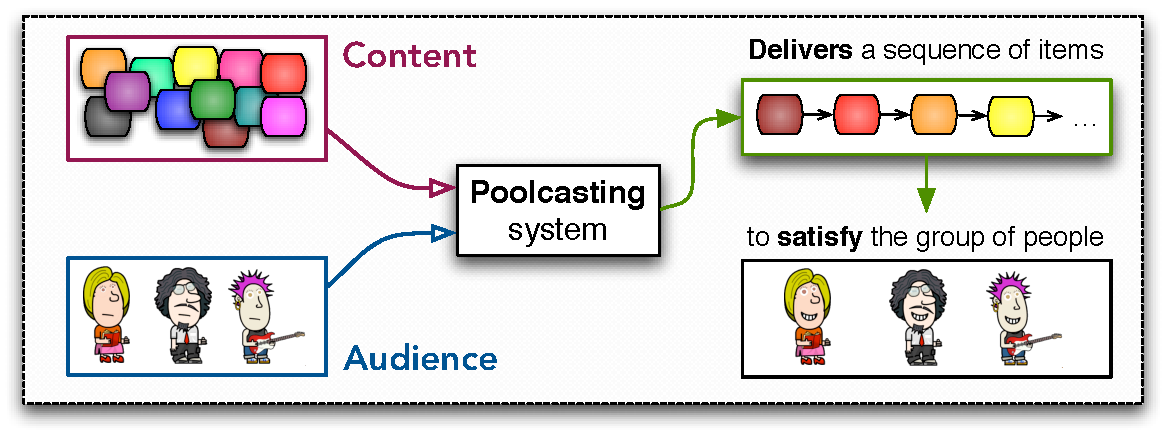
\epsfig{file=img/fig7_1, width=\textwidth}
\caption{A poolcasting system scenario.}
\label{fig:poolcasting-scenario}
\end{figure}

Poolcasting identifies a process that does not require human intervention and works sequentially, %(Fig.~\ref{fig:poolcasting_loop_channel}), 
selecting which items to deliver to the audience based on the previous items and on the preference and satisfaction of the audience.
Poolcasting can be considered, similarly to collaborative filtering, as a family of techniques applicable to user-adaptive systems.
%\begin{figure}[tbhp]
%\centering \setlength{\abovecaptionskip}{3pt}
%\epsfig{file=img/poolcasting_loop_channel2, width=\textwidth}
%\caption{The iterative process of a poolcasting channel.}
%\label{fig:poolcasting_loop_channel}
%\end{figure}

This dissertation has shown that reusing experiences collected from the Web to provide group-customised channels is a practical and productive research path.
Future work will be dedicated to investigate domains other than music where this approach can result effective.

\subsection{Generalising poolcasting} % (fold)
\label{sec:generalisation}

To extend poolcasting to other domains, it is important to summarise the fundamental features and requirements of the presented technique.

The first characteristic of poolcasting is its \emph{iterative} nature.
The goal of the technique is to generate a good \emph{sequence} of items\,---\,not just one\,---\,and for this reason a selection process is iterated multiple times.
At each iteration, poolcasting holds \emph{memory} of the previous selections to ensure that the whole sequence fulfils the desired requirements.

The second property of poolcasting is its \emph{social} nature.
The technique adapts content to a group\,---\,not an individual.
When members of a group have different preferences, poolcasting pursues fairness with a sequence that can possibly satisfy everyone at the same degree.
Poolcasting is designed for intentional groups, who accept to collaborate rather than to compete, for whatever reason that keeps the group alive.
The composition of the group can change over time and members can either be co-located or displaced.

The third characteristic is that domain knowledge comes from \emph{reusing past experiences}. % under a CBR view?
The principle is that the best way to customise content for a group is to learn from the way in which others have experienced that content in the past.
In particular, the focus is on the Web which offers the largest data source for human experiences.

The last relevant property is that poolcasting does not just \emph{recommend} but actually \emph{delivers} adapted content (e.g., broadcasting music on the Web), enabling the audience to share an actual experience and express immediate feedback which is valuable to improve customisation over time. 

\subsubsection{Poolcasting in the domain of movies} % (fold)
\label{sub:poolcasting_in_the_domain_of_movies}

One scenario where poolcasting could be useful is that of a family or a group of friends who meet weekly to watch movies together.
Each individual might have different `watching habits' and enjoy more or less different genres but still long for a social experience that reunites them week after week. % in front of a screen.

In this kind of situation, people implicitly accept the social compromise that they will probably not watch only movies they know and like, but will have the chance to discover titles enjoyed by their friends.

This scenario resembles that of Poolcasting Web radio, but the extension to the domain of movies requires some adjustments.
While songs in a radio are played one right after the other, movies are watched in separate days, therefore their order and continuity is not as relevant as in the case of music.

The satisfaction decay also changes: listening to three consecutive `less preferred' songs in a radio channel may be acceptable for an individual, since they would only count for 10 minutes of an entire music programme; watching three `less preferred' movies in a row, on the other hand, would be less acceptable, since they would correspond to three weeks of negative satisfaction for a specific individual.

Another difference resides in the data collected from the Web to identify associations. Working with movies requires to gather `watch-lists', sequences of titles watched by a person within a certain period.
Similarly to music, Web communities exist that make these data available for millions of users.

The co-occurrence analysis of these data is also different.
In the case of music, the simple fact of observing two songs occurring together in playlists suggests an association between them.
In the case of movies, an association can be derived only when many people watched the same two movies and \emph{rated them} identically.

A complete development of a movie-related poolcasting system remains future work, but preliminary studies suggest that the analysis of Web-mined data can produce good lists of top associated movies, as reported in Appendix~\ref{cha:appendix}.
%, similar to the lists of top associated songs and artists presented in Sect.~\ref{sub:the_smoothness_degrees_we_obtain}.

% Other domains will also be investigated, such as automatically selecting a sequence of interesting \emph{news items} for a group of displaced friends or deciding which \emph{TV shows} to broadcast for a `family prime-time' session. % sitting in front of a TV set.

\subsubsection{Poolcasting news items} % (fold)

Another promising scenario for poolcasting is delivering news items to a group of displaced friends.
Nowadays there is a clear discrepancy in the way in which news are produced and consumed.
Newspapers, newscasts and magazines force users to experience news in a fixed order, determined by the editorial board to satisfy an imaginary `average' consumer (e.g., first politics, then economics, then weather, then sport). 
However every person has a particular way of experiencing news; for instance one might flip through the first pages of a newspapers and skip directly to sport and weather.

Applying the poolcasting strategy to news items would mean to let people organise themselves in groups (\emph{news channels}) where they would specify their interests either explicitly (by means of genres, periods, tags) or implicitly (inferred from their previous experiences).
 
Within a channel, people would share news items with others and, in return, discover news that interest other like-minded persons. News producers would benefit from this model since they would be able to deliver the right \emph{content} to the right \emph{target}. 

Poolcasting news items would also blunt geographical constraints. 
People would be able to access their own `local news' channels, independently from their actual location. 
An Indian citizen living abroad, for instance, would still be able to receive daily updates about his hometown and become aware of news items prompted by his friends in India.

\subsubsection{Poolcasting TV programmes} % (fold)

A different domain where to apply poolcasting is that of a group of people, sitting together in front of a TV set, who have to decide which programmes to watch.
Thanks to PVRs (Personal Video Recorders), viewers can nowadays \emph{personalise} the order in which they wish to experience TV shows, but 
these systems only work for one person at the time and do not allow a \emph{group} to find a sequence of programmes that can satisfy everyone.

A common situation is that of a family where the father likes sport and action/comedy movies, the mother likes comedy movies and quiz shows, the grandmother likes documentaries and talk shows, the kid likes animated series and comedies: what programmes should they watch together?
Is there a social alternative to splitting the family into four separate screens?

The idea of a `poolcasting TV' consists in a system that autonomously configures prime-time TV group sessions day after day. 
This system would first build user profiles of each spectator, based on explicit feedback and observed behaviours (e.g., which shows each person tends to watch, at which time, for how long, when is the person at home).
During each session, the system would then aggregate multiple preferences, trying to satisfy the whole family in the long run.
For instance, one night the system might first broadcast an episode of an animated series, so the kid can happily go to sleep; then a documentary about sport legends, to generate an enriching discussion between father and grandmother; then a comedy movie, which would fairly satisfy all the adults.
Memory of past choices would help achieve balance and fairness among all the family members along time.

\subsection{Improving poolcasting} % (fold)
\label{sub:improving_the_quality_of_music_channels}

A different direction for future work deals with ways to improve the experience of members of poolcasting channels.

\subsubsection{Self-adaptive channels} % (fold)

A possible improvement to poolcasting is to introduce self-adaptive channels. These channels would diagnose decreases in performance and react accordingly, suggesting a solution to the participants. 

An example is given by the situation where a Poolcasting Web radio channel is listened by two discordant groups of listeners and the system has to struggle to adapt the music for the entire audience. 
In this case, a self-adaptive channel would detect the situation and suggest the two sub-groups to split into two separate channels, in order to maintain a higher degree of group satisfaction.

Introducing self-adaptive channels would be of great advantage to the participants. 
Self-adaptive channels can be seen as form of \emph{goal-driven learning} \cite{Leake93} as they would recognise situations where some type of failure occurs, access a library of possible correcting actions and then apply the best suited one to fix the problem. 

\subsubsection{Fuzzy affinity degrees} % (fold)
\label{ssub:smooth_genre_transitions}

A different direction to improve poolcasting experience is to enrich \emph{music ontology} from simple Boolean categories to fuzzy affinity degrees.

Poolcasting can currently categorise songs and artists in the music pool only in Boolean terms. 
Madonna, for instance, \emph{belongs to} the genre Pop and \emph{not to} the genres R\&B or Jazz. Likewise, Madonna \emph{has been tagged as} `female pop' and \emph{not as} `Spanish pop'.

The limitation of this representation becomes clear when poolcasting has to schedule music for multi-genre channels, for instance for a radio channel defined as `genre in (Pop, R\&B)'.
Ideally, a good musical selection for this channel would be to first play a song from the \emph{core} of a genre (e.g., a Pop song), then a series of songs \emph{in between} two genres (e.g., Pop/R\&B tracks) to finally reach a song in the core of the second genre and gradually move back to the first genre. %, and so on.
%
%Nevertheless, poolcasting cannot build such a sequence because it lacks the concepts of `core' and `in between' songs. 
%Poolcasting only knows which songs/artists belong to either genre, but not at which degree.
%
In order to achieve this behaviour, the music ontology employed by poolcasting has to be enriched to include \emph{fuzzy membership degrees}, to measure the \emph{degree} in which each song or artist belongs to each genre or tag. % (e.g., Madonna is 0.4 Pop, 0.8 R\&B, 0.3 Jazz, and so on). 
%For example, Madonna would not be characterised as Pop and not R\&B nor Jazz, but as a vector of fuzzy membership values [Pop = 0.4, R\&B = 0.8, Jazz = 0.3].

A method to describe songs and artists in terms of fuzzy membership degrees was introduced by the author in \cite{Baccigalupo08}.
Thanks to this method, artists can be characterised as vectors of fuzzy membership values rather than simply as Boolean categories. 
The music of Madonna, for instance, can be described as belonging to different genres at different fuzzy degrees: Pop (0.4), R\&B (0.8), Jazz (0.3), and so on.

%Integrating this approach into poolcasting would enable users to better define music channels, specifying whether they would like to hear only artists from the \emph{core} of a given genre (with high membership values) or whether they expect \emph{cross-genre} transitions to occur. 

Future work will be dedicated to embody the concept of ``genre affinity degree'' into poolcasting.
Users would benefit from this approach as they would be able to specify whether 
a channel should only play \emph{core} artists of a given genre (who show a high membership degree) or whether \emph{cross-genre} artists are allowed as well.

Poolcasting could also be able to better programme multi-genre radio channels, playing music that smoothly shifts from the core of a genre, to cross-genre songs, to songs belonging to a different genre and so on.
This improvement would make poolcasting behave more similarly to professional disc jockeys, who are able to swiftly transport music from a style/genre/tempo to a different one without disrupting transitions.



% subsubsection smooth_genre_transitions (end)


% subsection improving_the_quality_of_music_channels (end)
%\subsection{Fuzzy genres?} % (fold)
%\label{sub:fuzzy_genres_}

%boh
% subsection fuzzy_genres_ (end)

% section generalisation (end)


\section{Related publications} % (fold)
\label{sec:future_work}

The following papers were published as part of this research.

\begin{itemize}
    \item[] \cite{Baccigalupo06}
    C.~Baccigalupo and E.~Plaza.
    \newblock Case-based sequential ordering of songs for playlist recommendation.
    \newblock In T.~Roth-Berghofer, M.H. G{\"o}ker, and H.A. G{\"u}venir, editors, {\em Advances in {C}ase-{B}ased {R}easoning, Proceedings of the 8th European Conference on Case-Based Reasoning (ECCBR 2006)}, volume 4106 of {\em Lecture Notes in Computer Science}, pages 286--300. Springer, 2006.

      \item[] \cite{Baccigalupo07}
      C.~Baccigalupo and E.~Plaza.
      \newblock A case-based song scheduler for group customised radio.
      \newblock In R.~Weber and M.M. Richter, editors, {\em Case-{B}ased {R}easoning Research and Development, Proceedings of the 7th International Conference on Case-Based Reasoning (ICCBR 2007)}, volume 4626 of {\em Lecture Notes in Computer Science}, pages 433--448. Springer, 2007.

      \item[] \cite{Baccigalupo07c}
      C.~Baccigalupo and E.~Plaza.
      \newblock Mining music social networks for automating social music services.
      \newblock In {\em Workshop Notes of the ECML/PKDD 2007 Workshop on Web Mining 2.0}, pages 123--134, 2007.

      \item[] \cite{Baccigalupo07e}
      C.~Baccigalupo and E.~Plaza.
      \newblock Poolcasting: A social {W}eb radio architecture for group customisation.
      \newblock   In {\em Proceedings of the Third International Conference on Automated Production of Cross Media Content for Multi-Channel Distribution (AXMEDIS '07)}, pages 115--122. IEEE Computer Society, 2007.

      \item[] \cite{Baccigalupo07f}
      C.~Baccigalupo and E.~Plaza.
      \newblock Sharing and combining listening experience: a social approach to {W}eb radio.
      \newblock   In {\em Proceedings of the 2007 International Computer Music Conference (ICMC)}, pages 228--231, 2007.

      \item[] \cite{Baccigalupo08}
      C.~Baccigalupo, E.~Plaza, and J.~Donaldson.
      \newblock Uncovering affinity of artists to multiple genres from social behaviour data.
      \newblock In ISMIR \shortcite{ISMIR08}, pages 275--280.

      \item[] \cite{Plaza09}
      E.~Plaza and C.~Baccigalupo.
      \newblock Principle and praxis in the experience {W}eb: a case study in social music.
      \newblock In S.J. Delany, editor, {\em Proceedings of the ICCBR 2009
        Workshops}, pages 55--63. University of Washington Tacoma, 2009.


\end{itemize}

% SHOULD I ADD PRESENTATIONS? ECCBR06 industry, RECSYS 06 and ESTIU 2.0 ?


% mysql> select * from _all_movies_titles where title = "Boys Don't Cry" limit 3;
% +-------+------+----------------+
% | id    | year | title          |
% +-------+------+----------------+
% | 11880 | 2000 | Boys Don't Cry |
% | 12500 | 1999 | Boys Don't Cry |
% +-------+------+----------------+
% 2 rows in set (0.02 sec)
% 
% mysql> insert into customers_boys select distinct customer_id from ratings where movie_id = 12500;
% Query OK, 48419 rows affected (20.67 sec)
% 
% mysql> insert into ratings_boy select ratings.* from ratings join customers_boy using(customer_id);
% Query OK, 21406766 rows affected (221.07 sec)
% 
% mysql> insert into ratings_boy_boy select customer_id, date, rating from ratings_boy where movie_id = 12500;
% Query OK, 48419 rows affected (2.14 sec)
% 
% mysql> insert into ratings_boy_others_5days select r.movie_id, r.customer_id, datediff(r.date, s.date) from ratings_boy r join ratings_boy_boy s on r.customer_id = s.customer_id and r.rating = s.rating and abs(datediff(r.date, s.date)) <= 5 and movie_id <> 12500;
% Query OK, 1538594 rows affected (150.85 sec)
% 
% mysql> insert into frequency_boy_others_5days select movie_id, count(customer_id) as c, count_ratings, datediff from ratings_boy_others_5days join _most_rated_movies using(movie_id) group by movie_id, datediff;
% Query OK, 51443 rows affected (13.28 sec)
% 
% mysql> insert into results_boy_others_beta_08_d06 select movie_id, sum(pow(0.6, abs(datediff))*(coratings/20569)*pow(1-(popularity/479454), 0.8)) from frequency_boy_others_5days;
% Query OK, 1 rows affected (0.08 sec)
% 
% mysql> insert into results_boy_others_beta_08_d06 select movie_id, sum(pow(0.6, abs(datediff))*(coratings/20569)*pow(1-(popularity/479454), 0.8)) from frequency_boy_others_5days group by movie_id;
% Query OK, 8111 rows affected (0.10 sec)
% 
% mysql> select title, year, t from results_boy_others_beta_08_d06 join _all_movies_titles on movie_id = id order by t desc limit 10;

% NOTA: Ora nel MySQL ho la tabella che lista per ogni coppia di film il both_rated e both_best, ma % senza la distanza e l'ordine. Quindi dovrei avere questi dati, poi spiegare come l'ordine sia meno importante nei film, dato che sono piu' lunghi.. o forse anche togliere la distanza!!! 

% Quindi lo posso fare, basta fare cosi': se X = 175 e Y = 197
%d = select both_best from movies_to_movies_after100k where movie1_id = 175 and movie2_id = 197
%cx = select both_best from movies_to_movies_after100k where movie1_id = 175 and movie2_id = 175
%cy = select both_best from movies_to_movies_after100k where movie1_id = 197 and movie2_id = 197
%s = $\frac{d^{\beta + 1}}{cx \cdot cy^\beta}$

% subsection smoothness_in_movies (end)
 
% subsection customisation (end)





% section future_work (end)

% 

\bibliographystyle{named} 
\bibliography{bibliography} %\addcontentsline{toc}{chapter}{\bibname}

\appendix
\renewcommand{\@makechapterhead}[1]{\cleardoublepage\thispagestyle{empty}\vspace*{1\p@}%
  {\parindent \z@ \hyphenpenalty=10000 \centering \reset@font
        {\setromanfont{Minister Std Bold}
        \addfontfeature{LetterSpace=23.0}
        \thickhrulefill
        \begin{tabular}{|c|}    
%        {\quad{\bfseries\uppercase {#1}}\quad} >> For PROLOGUE
        {\bfseries\uppercase{Appendix \thechapter}}
        \end{tabular}}\thickhrulefill 
        \par\nobreak
        \vspace*{10\p@}%
        \interlinepenalty\@M
        \vspace*{10\p@}%
        \addfontfeature{LetterSpace=14.0}
        \LARGE\uppercase{#1}\par\nobreak
        \par
        \vspace*{5\p@}%
    %\vskip 40\p@
    \vskip 40\p@
  }}


\chapter{Top-associated movies}
\label{cha:appendix}
Preliminary experiments have shown that the analysis of watch-lists from the Web can return valuable lists of top associated movies, applying the same co-occurrence analysis process reported in Sect.~\ref{sec:co_occurrence_analysis5} to uncover associated songs.
The idea is that the more users have \emph{rented} the same two movies within a short period and have \emph{liked} them both, the more those movies are associated and can be recommended to people who have only watched one of the two. % Whenever a new user rents and likes one of the two movies, it makes sense to suggest the other one.

Experiments were run on a set of watch-lists obtained from the rental service company Netflix, which included 18,000 titles watched by over 480,000 users \cite{Bennett07}.
The watch-lists were analysed to identify pairs of movies watched by the same persons within a range of five days and both rated 5 out of 5 stars. 
Neither the order nor the distance between the movies were considered as relevant, corresponding to the parameters set to $\delta = 5$ (maximum distance in days), $\alpha_J = 0.2$ (distance not influent), $\gamma = 0.5$ (order not influent).
The popularity bias parameter was set to $\beta = 0.9$ to strongly punish over-popular movies in the watch-lists.

The result of the analysis was the compilation of lists of `top associated titles' according to Netflix users.
Each list reports titles loved by people who also rented and loved the `seed'  movie within a short period. 
Two sample lists of these `top associated titles' are reported hereafter.

\paragraph{Sense and sensibility (1995).} % (fold)
\label{par:sense_and_sensibility}

This movie was watched by 31,389 Netflix users. 
Within a period of five days, the same users also watched and equally rated 8,966 other movies.
%With a process equivalent to the one described for songs in Sect.~\ref{sec:co_occurrence_analysis5}, a movie-to-movie association was calculated from `Sense and Sensibility' to each of these movies, setting the parameters to $\delta = 5$ (maximum distance in days), $\alpha_J = 0.2$ (distance is not influent), $\gamma = 0.5$ (order is not influent), and $\beta = 0.9$ (over-popular movies are strongly punished).
The top associated movies uncovered were:
`Shakespeare in Love' (1998), `A Fish Called Wanda' (1988), `Amadeus' (1984), `The Full Monty' (1997) `Four Weddings and a Funeral' (1994), `Elizabeth' (1998), `Field of Dreams' (1989), `Much Ado About Nothing' (1993), `The Princess Bride' (1987), `Dead Poets Society' (1989).

\paragraph{Jumanji (1995).} % (fold)
\label{par:jumanji}

This movie was watched by 15,078 Netflix users. 
Within the same five days, these users also watched and assigned the same rating assigned to `Jumanji' to 7,406 other movies. 
The top associated movies turned out to be:
`Hook' (1991), `Kindergarten Cop' (1990), `Twister' (1996), `Flubber' (1997), `Beetlejuice' (1988), `Liar Liar' (1997), `Men in Black' (1997), `City Slickers' (1991), `A League of Their Own' (1992), `Father of the Bride' (1991).  


%Whenever new users rent and like the `seed' movie, it makes sense to suggest them a title in this list as they will probably going to like it as well.

% \paragraph{Tron (1982).} % (fold)
% \label{par:tron}
% 
% This movie has been watched by 20,569 Netflix users. The top associated movies turned out to be:
% `The Last Starfighter' (1984), `Willow' (1988), `The Abyss' (1989), `Highlander' (1986), `Clash of the Titans' (1981), `The Fifth Element' (1997), `Close Encounters of the Third Kind' (1977), `Star Trek II: The Wrath of Khan' (1982), `Time Bandits' (1981), `Total Recall' (1990).
% 


% \clearpage
% \pagestyle{index}
% %\renewcommand{\chaptermark}[1]{}
% \renewcommand{\preindexhook}{%
% The first page number is usually, but not always, the primary reference to
% the indexed topic.\vskip\onelineskip}
% \indexintoc
% \printindex
% 
\clearpage
\pagestyle{empty}
\null\vfil

\begin{adjustwidth}{1.15in}{1.15in}
\begin{center}
{\Large\    % \clearpage
{Colophon}}
\end{center}
\begin{center}
This thesis was typeset using the \LaTeX\;typesetting system created by Leslie Lamport and a memoir class. 

The graphs were plotted in R and designed with OmniGraffle Pro. 

The body text is set 11pt on a 369pt measure with Minister Std Light designed by Carl Albert Fahrenwaldt. 

Other font families include Helvetica, Avenir Std and Computer Modern.

\end{center}

\end{adjustwidth}

\vfil
\clearpage
 
\end{document}
